% % % % % % % % % % % % % % % % % % % % % % % % % % % % % % % % % % % % % % % % % % % % % % % 
%
%  Dokumentenvorlage für Abschlussarbeiten mit LaTeX (2021)
%    Institut für Technik und Informatik
%    Technische Hochschule Mittelhessen
%  
%  Version 0.8.0 - 17.06.21
%
%  Liste der Autor(en): 
%    - Jakob Czekansky ( jakob.czekansky@mni.thm.de )
% 
%  Wir freuen uns über jegliche Nutzung und weitere Verbesserungen.
%  
% % % % % % % % % % % % % % % % % % % % % % % % % % % % % % % % % % % % % % % % % % % % % % % 
% % % % % % % % % % % % % % % % % % % % % % % % % % % % % % % % % % % % % % % % % % % % % % % 
% 
%  WORKFLOW:
% 
%  Einfach 
%    - Ticket öffnen, 
%    - Merge-Request + Branch erstellen, 
%    - Änderungen einbringen, 
%    - Changelog (siehe unten) anpassen und
%    - Merge auf den development-Branch durchführen. 
%
% % % % % % % % % % % % % % % % % % % % % % % % % % % % % % % % % % % % % % % % % % % % % % % 
% % % % % % % % % % % % % % % % % % % % % % % % % % % % % % % % % % % % % % % % % % % % % % % 
%
%  Changelog: 
%    - ... [next entry, please] 
%    - add initial LaTeX project (v0.8.0, 17.06.21)
%    
% % % % % % % % % % % % % % % % % % % % % % % % % % % % % % % % % % % % % % % % % % % % % % % 



\documentclass[	12pt,
				a4paper,
				bibliography=totoc,
				listof=totoc,
				index=totoc,
				twoside,
				headsepline,
				footsepline,
				ngerman]{scrartcl}

\usepackage[ngerman]{babel}
\usepackage{blindtext}
%\usepackage{titlesec}
\setcounter{secnumdepth}{4}
\usepackage{breakcites}
\usepackage[utf8]{inputenc}
\usepackage{amsmath}
\usepackage{amsfonts}
\usepackage{amssymb}
\usepackage{graphicx}
\usepackage[automark]{scrpage2}
%\usepackage{fancyhdr}
\usepackage{tabularx}
%\usepackage[showframe]{geometry}
\usepackage{geometry}
\usepackage{setspace}
\usepackage[right]{eurosym}
\usepackage[printonlyused]{acronym}
\usepackage{subfig}
\usepackage{floatflt}
\usepackage[usenames,dvipsnames]{color}
\usepackage{colortbl}
\usepackage{paralist}
\usepackage{array}
\usepackage{color}
\usepackage{xcolor}
\usepackage{caption}
\usepackage{url}
\usepackage{svg}
\def\UrlBreaks{\do\/\do-}

\usepackage{parskip}
\usepackage[right]{eurosym}
%\usepackage{picins}
\usepackage[subfigure,titles]{tocloft}
\usepackage[pdfpagelabels=true, breaklinks=true]{hyperref}
\usepackage{verbatim}
\usepackage{hyperref}
%\usepackage[euler]{textgreek}
%\usepackage{chngcntr}
%\counterwithout{footnote}{section}
%\usepackage{perpage} \MakePerPage{footnote}
\usepackage{multibbl}
\usepackage{multirow}
\usepackage{mathtools}
\usepackage{wrapfig}
\usepackage{pdflscape}
\usepackage{imakeidx}
\usepackage{scrextend}
\usepackage{varwidth}
\usepackage{tablefootnote}
\usepackage{pgfplots}
\usepackage{nicefrac}
%\usepackage{siunitx}  
\usepackage{todonotes}

%\usepackage{showframe}
%\renewcommand*\ShowFrameColor{\color{red}}

\captionsetup[table]{skip=0pt}

\usepackage{svg}
\usepackage[absolute,overlay]{textpos}
\usepackage{enumitem}
\indexsetup{firstpagestyle=headings}
%\makeindex
\makeindex[columns=2, options=-s mystyle]

\usepackage{filecontents}
\begin{filecontents}{mystyle.ist}
	headings_flag  1 % wir benutzen Überschriften
	heading_prefix "{\\bfseries " % und setzen sie fett
	heading_suffix "\\hfil}\\nopagebreak\n"% und links, nach ihnen kein Seitenumbruch
	delim_0 "\\dotfill" % Punktzeile zwischen Einträgen und Seitenzahlen (Ebene 0)
	delim_1 "\\dotfill" % Punktzeile zwischen Einträgen und Seitenzahlen (Ebene 1)
	delim_2 "\\dotfill" % Punktzeile zwischen Einträgen und Seitenzahlen (Ebene 2)
	delim_r "--" % Trenner zwischen Start Kalman-Filterund Ende eines Seitenbereiches
	suffix_2p "\\,f." % Suffix bei einem bereich aus 2 Seiten
	suffix_3p "\\,ff." % Suffix bei einem bereich aus 3 Seiten
\end{filecontents}

\usepackage{subfiles}

\DeclarePairedDelimiter{\ceil}{\lceil}{\rceil}
\DeclarePairedDelimiter{\floor}{\lfloor}{\rfloor}


\newbibliography{all}

\newcolumntype{L}[1]{>{\raggedright\arraybackslash}p{#1}} % linksbündig mit Breitenangabe
\newcolumntype{C}[1]{>{\centering\arraybackslash}p{#1}} % zentriert mit Breitenangabe
\newcolumntype{R}[1]{>{\raggedleft\arraybackslash}p{#1}} % rechtsbündig mit Breitenangabe


\setcounter{secnumdepth}{4}
\setcounter{tocdepth}{4}

%fuer Listings
\usepackage{listings}

\begin{comment}
\lstset{literate=
	{á}{{\'a}}1 {é}{{\'e}}1 {í}{{\'i}}1 {ó}{{\'o}}1 {ú}{{\'u}}1
	{Á}{{\'A}}1 {É}{{\'E}}1 {Í}{{\'I}}1 {Ó}{{\'O}}1 {Ú}{{\'U}}1
	{à}{{\`a}}1 {è}{{\`e}}1 {ì}{{\`i}}1 {ò}{{\`o}}1 {ù}{{\`u}}1
	{À}{{\`A}}1 {È}{{\'E}}1 {Ì}{{\`I}}1 {Ò}{{\`O}}1 {Ù}{{\`U}}1
	{ae}{{\"a}}1 {ë}{{\"e}}1 {ï}{{\"i}}1 {oe}{{\"o}}1 {ue}{{\"u}}1
	{Ä}{{\"A}}1 {Ë}{{\"E}}1 {Ï}{{\"I}}1 {Ö}{{\"O}}1 {Ü}{{\"U}}1
	{â}{{\^a}}1 {ê}{{\^e}}1 {î}{{\^i}}1 {ô}{{\^o}}1 {û}{{\^u}}1
	{Â}{{\^A}}1 {Ê}{{\^E}}1 {Î}{{\^I}}1 {Ô}{{\^O}}1 {Û}{{\^U}}1
	{œ}{{\oe}}1 {Œ}{{\OE}}1 {æ}{{\ae}}1 {Æ}{{\AE}}1 {ss}{{\ss}}1
	{ű}{{\H{u}}}1 {Ű}{{\H{U}}}1 {ő}{{\H{o}}}1 {Ő}{{\H{O}}}1
	{ç}{{\c c}}1 {Ç}{{\c C}}1 {ø}{{\o}}1 {å}{{\r a}}1 {Å}{{\r A}}1
	{€}{{\euro}}1 {£}{{\pounds}}1 {«}{{\guillemotleft}}1
	{»}{{\guillemotright}}1 {ñ}{{\~n}}1 {Ñ}{{\~N}}1 {¿}{{?`}}1
}
\end{comment}

\definecolor{mGreen}{rgb}{0,0.6,0}
\definecolor{mGray}{rgb}{0.5,0.5,0.5}
\definecolor{mPurple}{rgb}{0.58,0,0.82}
\definecolor{backgroundColour}{rgb}{0.95,0.95,0.92}
\definecolor{light-gray}{gray}{0.90}

\definecolor{mygreen}{rgb}{0,0.6,0}
\definecolor{mygray}{rgb}{0.5,0.5,0.5}
\definecolor{mymauve}{rgb}{0.58,0,0.82}

\definecolor{THM-green-CMYK}{cmyk}{57,0,100,0}
\definecolor{THM-green-HTML}{HTML}{80ba24}

\definecolor{THM-gray-CMYK}{cmyk}{33,4,0,72}
\definecolor{THM-gray-HTML}{HTML}{4a5c66}

\definecolor{THM-yellow-CMYK}{cmyk}{0,30,100,0}
\definecolor{THM-yellow-HTML}{HTML}{f4aa00}

\definecolor{THM-red-CMYK}{cmyk}{0,100,65,28}
\definecolor{THM-red-HTML}{HTML}{9c132e}

\definecolor{THM-cyan-CMYK}{cmyk}{75,0,7,0}
\definecolor{THM-cyan-HTML}{HTML}{00b8e4}

\definecolor{THM-blue-CMYK}{cmyk}{100,72,0,18}
\definecolor{THM-blue-HTML}{HTML}{002878}

\definecolor{table-green}{HTML}{80ba24}%66FF66}
\definecolor{table-yellow}{HTML}{f4aa00}%{FFFF33}
\definecolor{table-red}{HTML}{9c132e}%{FF6666}

\definecolor{table-font-color}{HTML}{FFFFFF}


\definecolor{code-green}{HTML}{0C7A20}

\lstset{ %
	backgroundcolor=\color{white},   % choose the background color; you must add \usepackage{color} or \usepackage{xcolor}; should come as last argument
	basicstyle=\footnotesize,        % the size of the fonts that are used for the code
	breakatwhitespace=false,   	     % sets if automatic breaks should only happen at whitespace
	breaklines=true,                 % sets automatic line breaking
	captionpos=t,                    % sets the caption-position to bottom
	commentstyle=\color{mygreen},    % comment style
	deletekeywords={...},            % if you want to delete keywords from the given language
	escapeinside={\%*}{*)},          % if you want to add LaTeX within your code
	extendedchars=true,              % lets you use non-ASCII characters; for 8-bits encodings only, does not work with UTF-8
	frame=single,	                   % adds a frame around the code
	keepspaces=true,                 % keeps spaces in text, useful for keeping indentation of code (possibly needs columns=flexible)
	keywordstyle=\color{blue},       % keyword style
	language=C,                 % the language of the code
	morekeywords={*,...},            % if you want to add more keywords to the set
	numbers=left,                    % where to put the line-numbers; possible values are (none, left, right)
	numbersep=5pt,                   % how far the line-numbers are from the code
	numberstyle=\tiny\color{mygray}, % the style that is used for the line-numbers
	rulecolor=\color{black},         % if not set, the frame-color may be changed on line-breaks within not-black text (e.g. comments (green here))
	showspaces=false,                % show spaces everywhere adding particular underscores; it overrides 'showstringspaces'
	showstringspaces=false,          % underline spaces within strings only
	showtabs=false,                  % show tabs within strings adding particular underscores
	stepnumber=1,                    % the step between two line-numbers. If it's 1, each line will be numbered
	stringstyle=\color{mymauve},     % string literal style
	tabsize=2,	                  	 % sets default tabsize to 2 spaces
	title=\lstname,                   % show the filename of files included with \lstinputlisting; also try caption instead of title
}
\renewcommand{\ttdefault}{pcr}
\renewcommand{\lstlistingname}{Code}

\definecolor{code-green}{HTML}{005032}
\definecolor{code-purple}{HTML}{7F0055}

\lstdefinestyle{customc}{
	belowcaptionskip=0.3\baselineskip,
	breaklines=true,
	%xleftmargin=\parindent,
	language=C,
	captionpos=b,
	showstringspaces=false,
	basicstyle=\small\ttfamily,
	keywordstyle= {\bfseries\color{code-purple}},
	keywordstyle = [2]{\color{code-green}},
	commentstyle=\itshape\color{purple!40!black},
	identifierstyle=\color{black},
	stringstyle=\color{orange},
	morekeywords={*,...},
	morekeywords = [2]{uint32_t,uint16_t,uint8_t, int16_t, ODOMETER_DATA},
}

\lstset{basicstyle=\footnotesize\bfseries, captionpos=b, breaklines=true, showstringspaces=false, tabsize=2, frame=lines, numbers=left, numberstyle=\tiny, xleftmargin=2em, framexleftmargin=2em}
%\color{THM-green-HTML}


\definecolor{light-gray}{gray}{0.8}

\newcommand{\inlinecode}[1]{\lstset{style=customc}{\lstinline[columns=fixed]{#1}}}
%\newcommand{\inlinecode}[1]{\textit{#1}}
\newcommand{\nfl}{\newline\hspace*{-0.47em}}

\newcommand{\reference}[1]{\textit{\ref{#1} \nameref{#1}}}

\makeatletter

\def\l@lstlisting#1#2{\@dottedtocline{1}{0em}{1.95em}{\hspace{1,15em} Code #1}{#2}}
\makeatother

\newcommand{\includecode}[1]{\lstinputlisting[caption= #1]{#1}}

% Quellenverweise für Grafiken
\newcommand{\captionsource}[1]{\itshape\footnotesize (#1)}

%\renewcommand{\autoref}[1]{\textit{\autoref{#1}}}

\renewcommand{\labelitemi}{$\bullet$}
\renewcommand{\labelitemii}{\small$\circ$}
\renewcommand{\labelitemiii}{\small$\circ$}
\renewcommand{\labelitemiv}{$\circ$}

%Seitenraender
\geometry{a4paper, top=27mm, left=30mm, right=20mm, bottom=35mm, headsep=10mm, footskip=12mm}

%Links und PDF-Einstellungen
\hypersetup{unicode=false, pdftoolbar=true, pdfmenubar=true, pdffitwindow=false, pdfstartview={FitH},
	pdftitle={Titel der Arbeit},
	pdfauthor={AUTOR:IN},
	pdfsubject={Bachelorarbeit}, % / Masterarbeit
	pdfcreator={\LaTeX\ with package \flqq hyperref\frqq},
	pdfproducer={pdfTeX \the\pdftexversion.\pdftexrevision},
	pdfkeywords={Institut für Technik und Informatik, Technische Hochschule Mittelhessen},
	pdfnewwindow=true,
	colorlinks=true,
	linkcolor=black,
	citecolor=black,
	filecolor=magenta,
	urlcolor=black,
	linktoc=all}
\pdfinfo{/CreationDate (D:20110620133321)}

\newcommand{\subfigureautorefname}{\figureautorefname}

\begin{document}

% ----------------------------------------------------------------------------------------------------------
% Titelseite
% ----------------------------------------------------------------------------------------------------------
% ----------------------------------------------------------------------------------------------------------
% Titelblatt
% ----------------------------------------------------------------------------------------------------------
\thispagestyle{empty}
\begin{center}
	
\includegraphics[height=1.7cm]{img/thm-logo/thm1.png}
	\hfill
	
\includegraphics[height=1.7cm]{img/iti-logo/iti_2020_whitespace.png}\\
	
	\vfill
	
	\Huge
	\textbf{Bachelorarbeit}\\ % / Masterarbeit	
		
	\vfill
	
	\Huge
	\textit{Entwicklung eines Lasertriangulationssensor zur Oberflächen-Rekonstruktion mit ROS2}\\
	
	\vfill
	
	\large	
	zur Erlangung des akademischen Grades  \\
	
	\vfill
	
	\textbf{Bachelor of Science (B.Sc.)}\\ % Master of Science (M.Sc.)
	
	\vfill
	
	vorgelegt dem  \\
	
	\vfill
	
	Fachbereich Mathematik, Naturwissenschaften und Informatik \\	
	der Technischen Hochschule Mittelhessen. \\
	
	\vfill
	
	\textbf{Tristan Elias Wolfram}\\
	
	\vfill
	
	\normalsize
	\text{27.05.2022, Gießen}\\
	
	\vfill

	\begin{tabular}{rl}
		\rule{0mm}{2ex}\textbf{Referentin:}    	& Prof. Dr.-Ing. Seyed Eghbal Ghobadi\\ 
		\rule{0mm}{2ex}\textbf{Korreferent:} 	& Moritz Schauer, M.Sc. \\ 
	\end{tabular} 
\end{center}
\cleardoublepage


\onehalfspacing
\pagestyle{scrheadings}
\pagenumbering{Roman}

% ----------------------------------------------------------------------------------------------------------
% Abstract / Kurzfassung
% ----------------------------------------------------------------------------------------------------------
% ----------------------------------------------------------------------------------------------------------
% Kurfassung / Abstract
% ----------------------------------------------------------------------------------------------------------
\section*{Titel}
Entwicklung eines Lasertriangulationssensors zur Oberflächen-Rekonstruktion mit ROS2
\vfill
\subsubsection*{Kurzfassung}

Oberflächenrekonstruktion findet in der Industrie weitreichend ihre Anwendung. Sei es um kleine Bauteile zu untersuchen, größere Objekte auf Schäden zu prüfen oder auch ganze Landstriche zu vermessen. Dabei ist die Lasertriangulation eine gängige Methode, um 3D-Informationen zu erhalten. Diese Arbeit beschäftigt sich mit einem Open-Source entwickelten Lasertriangulationssensor. Dieser Sensor soll in einem an dem Institut für Technik und Informatik (ITI) durchgeführten Forschungsprojekt eingesetzt werden. Die Aufgabe dabei ist, von Holzscheiben eine 3D-Aufnahme mit zusätzlichen Farbinformationen zu erzeugen. In dieser Arbeit werden die Entwicklung und Umsetzung selbst, aber auch die mathematischen Grundlagen erläutert. Die Ergebnisse werden evaluiert und mit dem aktuellen Standard verglichen.

\section*{Title}
Development of a laser triangulation sensor for surface reconstruction with ROS2

\vfill
\subsubsection*{Abstract}

Surface reconstruction is widely used in industry. Be it for inspecting small components, checking larger objects for damage or even surveying entire areas. Laser triangulation is a common method for obtaining 3D information. This thesis deals with an open-source developed laser triangulation sensor. This sensor will be used in a research project at the Institut für Technik und Informatik (ITI). The task here is to generate a 3D image of wooden slices with additional color information. In this paper the development and implementation itself, but also the mathematical basics are explained. The results are evaluated and compared with the current standard.

\clearpage


\renewcommand{\cfttabpresnum}{Tab. }
\renewcommand{\cftfigpresnum}{Abb. }
\settowidth{\cfttabnumwidth}{Abb. 10\quad}
\settowidth{\cftfignumwidth}{Abb. 10\quad}

% ----------------------------------------------------------------------------------------------------------
% Inhaltsvezeichnis
% ----------------------------------------------------------------------------------------------------------
\thispagestyle{empty}
~
\newpage
\tableofcontents

\newpage
\thispagestyle{empty}
~
\clearpage

% ----------------------------------------------------------------------------------------------------------
% Danksagung
% ----------------------------------------------------------------------------------------------------------
% ----------------------------------------------------------------------------------------------------------
% Danksagung
% ----------------------------------------------------------------------------------------------------------
\ohead{Danksagung}
\section*{Danksagung}
An dieser Stelle kann man Danke sagen. :-)
\vfill
\begin{center}
	\Large
	DANKE
\end{center}
\vfill

\newpage
\cleardoublepage

\pagenumbering{arabic}
\ohead{\rightmark}

% ----------------------------------------------------------------------------------------------------------
% Einleitung
% ----------------------------------------------------------------------------------------------------------
% ----------------------------------------------------------------------------------------------------------
% Die Einleitung
% ----------------------------------------------------------------------------------------------------------
\section{Einleitung}\label{einleitung}
Die Möglichkeit eine Oberfläche in ihrer Beschaffenheit dreidimensional zu erfassen, birgt viele Anwendungsfälle. Sei es, um ein 3D-Abbild von einem Raum digital zu erhalten oder in der Industrie Bauteile zu vermessen und auf Fehler zu prüfen. Dabei sind viele verschiedene Verfahren über die Zeit entwickelt und optimiert wurden. 3D Kameras oder auch RGB-D Kameras finden heute vielfältig ihren Einsatz. Diese Arbeit beschäftigt sich mit der Dokumentation und Evaluation eines im Rahmen meiner Praktikumsphase an der Technischen Hochschule Mittelhessen entwickelten Lasertriangulationssensor. Ziel dieser Arbeit ist es, die Funktionalität und Architektur dieses Sensors zu erklären. Zusätzlich soll der Sensor evaluiert und auf bestimme Aspekte mit dem aktuellen Stand der Technik im Bereich der 3D-Kameras bzw. RGB-D Kameras verglichen werden.
Sinn und Zweck eines Lasertriangulationssensor ist es, eine Oberfläche zu rekonstruieren und dabei nicht nur die Tiefen-Informationen, sondern auch die Farbinformationen gemeinsam aufzunehmen. Als Verfahren wird, wie im Namen genannt, die Lasertriangulation verwendet.

	\subsection{Aufgabe - Motivation}
	Die grundsätzliche Aufgabe und Motivation entstand durch ein Projekt in Zusammenarbeit mit der Firma RINNTECH – „Technik zur Prüfung von Bäumen“. Die Firma bezeichnet sich selbst wie folgt: „Als Anwender und Entwickler verfügen wir über jahrelange Erfahrung und zahlreiche Patente auf dem Gebiet der Baum- und Holzanalyse. Für diese Anforderungen können wir Ihnen daher ausgereifte Technik und umfassenden Service anbieten“ \citep[vgl.][]{noauthor_rinntech_nodate}. Beispielanwendungen, für die Geräte und Software bereitgestellt werden sind zum Beispiel Bäume kontrollieren, Jahrringe analysieren, Holzkonstruktionen kontrollieren und Holzqualität und Zuwachs im Wald kontrollieren \citep[vgl.][]{noauthor_rinntech_nodate}. Das zugrundeliegende Projekt wurde als Forschungs- und Entwicklungsprojekt zusammen mit dem Institut für Technik und Informatik (ITI) an der THM gestartet. Es trägt den Titel
	
	\textit{\glqq Entwicklung einer Messmethodik zur Ermöglichung einer schnellen Bestimmung von Holzart und -herkunft anhand von Jahrring- und Farbanalyse. Entwicklung der Messwerterfassung und -auswertung der neuen Messmethodik\grqq}
	
	und beschäftigt sich konkret mit der Jahrringanalyse. Durch diese soll Holzart und Herkunft bestimmt werden. RINNTECH verkauft das Produkt „LINTAP“ für diesen Zweck \citep[vgl.][Produkte]{noauthor_rinntech_nodate}. Das schon existierende Produkt soll in dem Projekt erweitert, optimiert und automatisiert werden. Die Grundidee besteht darin, dass sich ein Roboter-Arm mit einer hochauflösenden Kamera über das Objekt bewegt und entsprechende Bilder aufnimmt, die für die Jahrringanalyse erforderlich sind. Hier wird eine Kamera eingesetzt, die von dem Roboterarm nah an das Holz herangeführt werden muss. Die Pfade, die der Roboter dementsprechend abfahren soll, müssen also mit hinreichender Genauigkeit errechnet werden. Dazu ist eine digitale Abbildung des Holzes unverzichtbar. Anhand einer rekonstruierten Oberfläche können die entsprechenden Pfade für den Roboter ohne Probleme bestimmt werden. Es muss also initial eine Oberflächen-Rekonstruktion des Objektes stattfinden. An diesem Punkt setzt diese Arbeit an. Es wurde eine Software entwickelt, die mithilfe einer Kamera und eines Linienlasers einen 3D-Scan durchführt. Dabei werden die Tiefeninformationen und auch die Farbinformationen aufgenommen und verarbeitet. Man erhält eine Punktewolke der gescannten Oberfläche, die entsprechend eingefärbt ist. Hierbei handelt es sich um einen typischen Output für eine 3D-Kamera in der Industrie. Die Aufgabenstellung wurde noch etwas konkretisiert. Als Methode soll die Lasertriangulation verwendet werden. Dazu wurde eine Kamera und ein Linienlaser bereitgestellt. Zusätzlich soll nur Open-Source-Software verwendet werden und die Anwendung muss über ROS2 (Robot Operating System) laufen.
	
	\subsection{Stand der Technik}
		\subsubsection{Methodik}
		Lasertriangulation ist nicht die einzige Methode, eine Oberflächen-Rekonstruktion durchzuführen. Die zentralen Technologien zu diesem Zweck sind Triangulation oder Time-of-Flight \citep[vgl.][]{zollhofer_state_2018}. 
		Bei der Triangulation gibt es zwei Ansätze. Ein Ansatz ist der Direkte über Structured Light. Dabei wird ein bekanntes Muster mit einem Laser oder Ähnlichem auf die Oberfläche projiziert. Eine Kamera nimmt das Muster als Bild auf, welches sich durch die variierende Höhe und Form der Oberfläche verzerrt. Diese Verzerrung wird als Anhaltspunkt verwendet, um die Unterschiedlichkeiten in der Höhe zu ermitteln. Lasertriangulation, der hier verwendete Lösungsansatz, ist diesem Ansatz zuzuordnen. \newline
		Einen indirekten Ansatz der Triangulation bietet Stereo-Vision. Dabei werden zwei Kameras verwendet, die zwei aufgenommene Bilder aus unterschiedlichen Positionen liefern. Ebenfalls wird ein fester Punkt benötigt, der auch mit einem Laser oder Ähnlichem im Bild projiziert werden kann. Über die zwei unterschiedlichen Bilder kann die Position ermittelt werden.
		
		Die Time-of-Flight-Technologie benutzt eine andere Lösungsmöglichkeit. Es wird Licht auf einen Punkt auf der Oberfläche gestrahlt. Dort wird es zurück reflektiert und von einem Sensor registriert. Dieser misst die verstrichene Zeit. Durch die bekannte Geschwindigkeit von Licht, kann über die gebrauchte Zeit der zurückgelegte Weg errechnet werden. Dieser entspricht der Höhe.
	
		\subsubsection{Geräte}
		Diese Methoden finden ihre Anwendung auch in der Industrie. Diverse Geräte und Anwendungen zur Oberflächen-Rekonstruktion sind bereits auf dem Markt. Die Rede ist von sogenannten 3D-Kameras bzw. RGB-D Kameras. Dabei steht RGB (Red, Green, Blue) für die Farbinformationen und das D (Depth) für die Tiefeninformation. Angefangen mit der von Microsoft entwickelten „Kinect“ über die „Intel RealSense“ zur „Google Tango“ folgen viele weitere Geräte. Diese sind nicht nur meist für einen geringen Preis verfügbar, sie könne auch die entsprechenden Pixelfarben in einer hohen Auflösung aufnehmen.
		Zusätzlich geschieht die Aufnahme in Echtzeit, was bedeutet, dass sich die herausgegebene Punktewolke ändert, sobald sich die aufgenommene Oberfläche ändert bzw. die Kamera bewegt wird \citep[vgl.][]{state_of_art_zoll}.
			
	\subsection{Anforderungen}
	Für das Projekt wurde zu Beginn eine „Intel RealSense d415“ verwendet. Die Industrie-3D-Kamera erfüllt die Anforderungen. Es kann eine 3D-Rekonstruktion des Objektes mit Farbinformationen durchgeführt werden. Die RealSense verwendet Stereo-Vision-Technologie. Sie verfügt über zwei Kameras und einen Projektor für ein vom Menschen nicht sichtbares Infrarot-Muster. Die Kamera berechnet so für jeden Pixel seine 3D-Position in Echtzeit. In dem Forschungsprojekt wurde jedoch auch überlegt, ob man die 3D-Rekonstruktion jenseits eine Industrie-Lösung erhalten kann. Grundsätzlich ist dafür eine einfache Webcam mit einem Linienlaser ausreichend. So kam die Idee, einen Open-Source Lasertriangulationssensor zu entwickeln.
	Dieser soll mit der Intel RealSense und dem generellen Industriestandart von RGB-D Kameras verglichen werden. Dabei ist die Genauigkeit (der Tiefeninformationen), Schnelligkeit des Scans und die Auflösung der Farbinformationen ausschlaggebend. Sowohl die Intel RealSense als auch die Open-Source-Variante sollen am Ende eine Punktewolke liefern. Diese kann im Vergleich analysiert werden. Genauso können die Position der Punkte auf eine Genauigkeit hin untersucht werden.
	\newpage
	
	\subsection{Lösungsansatz}
	Um den genaueren Erklärungen im Hauptteil folgen zu können, soll einmal oberflächlich der Lösungsansatz der entwickelten Anwendung erläutert werden. Die grundlegende Idee ist die Lasertriangulation. Dafür ist eine Kamera und ein Projektor für eine Laserlinie notwendig.
	\begin{figure}[h]
		\centering
		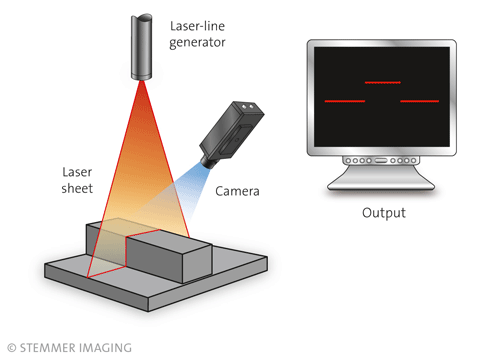
\includegraphics[width=0.7\linewidth]{img/grundlagen/lasertriangulation_1}
		\caption{Lasertriangulation}
		\captionsource{Abbildung entnommen aus \citep{noauthor_3d-bildverarbeitung_nodate}}
		\label{fig:lasertriangulation}
	\end{figure}

	Die resultierende Punktewolke der 3D-Rekonstruktion muss im Bezug zu einem Koordinatensystem stehen. Als Bezugspunkt wird die Kamera gewählt. Das bedeutet, dass sich die Koordinaten auf die Kamera beziehen und sich der Ursprung des Koordinatensystems an den optischen Sensor der Kamera befindet. Für die Berechnung von einem Pixel zu einem 3D-Punkt wird die Ebene bestimmt, die der Laser projiziert. Ausgehend von dem Startpunkt des Projektors und der projizierten Linie kann das Laserlicht als Ebene begriffen werden. In Abb. (\ref{fig:lasertriangulation}) ist diese rot ausgefüllt. Diese Ebene kann aus Kamerasicht als Ebenengleichung dargestellt und errechnet werden. In der Theorie wird dann, sobald die Ebenengleichung bekannt ist, eine Laserlinie auf die zu scannende Oberfläche projiziert. Die Kamera nimmt ein Bild von dieser Oberfläche auf. Über diverse Bildverarbeitungs-Operationen wird aus dem aufgenommenen Bild die rote Laserlinie herausgearbeitet. In Abb. (\ref{fig:lasertriangulation}) wird unter \emph{Output} beispielhaft das Ergebnis dieses Prozesses gezeigt. Die Pixel der Laserlinie werden im nächsten Schritt auf die Ebene gespannt, indem sie in die Ebenengleichung eingesetzt werden. Dadurch wird eine dritte Dimension für die Pixel errechnet. Die 3D-Punkte sind dann, wie gefordert, aus Sicht der Kamera. Diese Methodik liefert die 3D-Repräsentation der Laserlinie, jedoch nicht von dem kompletten Objekt. Der Sensor (bestehend aus der Kamera, dem Laser und der Software zusammen) muss zusätzlich über das Objekt bewegt werden. Die aufgenommenen Linien werden dann zu einer gesamten Punktewolke zusammengefügt. Dabei muss bekannt sein, welche Strecke an Bewegung von dem Sensor zurückgelegt wurde, um die neue Linie in der richtigen Position einzufügen. 

\clearpage
% ----------------------------------------------------------------------------------------------------------
% Stand der Technik
% ----------------------------------------------------------------------------------------------------------
%% ----------------------------------------------------------------------------------------------------------
% Stand der Technik
% ----------------------------------------------------------------------------------------------------------
\section{Stand der Technik}\label{stand-der-technik}
	\subsection{Methodik}
	Lasertriangulation ist nicht die einzige Methode eine Oberflächen-Rekonstruktion durchzuführen. Die zentralen Technologien zu diesem Zweck sind Triangulation oder Time-of-Flight [Vgl.: SotA]. 
	Bei der Triangulation gibt es zwei Ansätze. Einen direkten über Structured Light. Dabei wird ein bekanntes Muster mit einem Laser oder Ähnlichem auf die Oberfläche projiziert. Eine Kamera nimmt das Muster als Bild auf, welches sich durch die variierende Höhe und Form der Oberfläche verzerrt. Diese Verzerrung wird als Anhaltspunkt verwendet, um die Unterschiedlichkeiten in der Höhe zu ermitteln. Lasertriangulation und der hier verwendete Lösungsansatz gehören zu dieser Möglichkeit. 
	Einen indirekten Ansatz der Triangulation bietet Stereo-Vision. Dabei werden zwei Kameras verwendet, die zwei aufgenommenen Bildern aus unterschiedlichen Positionen liefern. Ebenfalls wird ein fester Punkt benötigt, der auch mit einem Laser oder Ähnlichem im Bild projiziert werden kann. Über die zwei unterschiedlichen Bilder kann die Position ermittelt werden.
	
	Die Time-of-Flight-Technologie benutzt eine andere Lösungsmöglichkeit. Es wird Licht auf einen Punkt auf der Oberfläche gestrahlt. Dort wird es zurück reflektiert und von einem Sensor registriert. Dieser misst die verstrichene Zeit. Durch die bekannte Geschwindigkeit von Licht, kann über die gebrauchte Zeit der zurückgelegte Weg errechnet werden. Dieser entspricht der Höhe.

	\subsection{Geräte}
	Diese Methoden finden ihre Anwendung auch in der Industrie. Diverse Geräte und Anwendungen zur Oberflächen-Rekonstruktion sind bereits auf dem Markt. Die Rede ist von sogenannten 3D-Kameras bzw. RGB-D Kameras. Dabei steht RGB (Red, Green, Blue) für die Farbinformationen und das D (Depth) für die Tiefeninformation. Angefangen mit der von Microsoft entwickelten „Kinect“ über die „Intel RealSense“ zur „Google Tango“ folgen viele weitere Geräte. Diese sind nicht nur meist für einen geringen Preis verfügbar, sie könne auch die entsprechenden Pixelfarben in einer guten Auflösung aufnehmen. Zusätzlich geschieht die Aufnahme in Echtzeit, was bedeutet, dass sich die herausgegebene Punktewolke ändert, sobald sich die aufgenommene Oberfläche ändert bzw. die Kamera bewegt wird.

%\clearpage

% ----------------------------------------------------------------------------------------------------------
% Grundlagen
% ----------------------------------------------------------------------------------------------------------
% ----------------------------------------------------------------------------------------------------------
% Die Grundlagen
% ----------------------------------------------------------------------------------------------------------
\section{Grundlagen}\label{grundlagen}
	Um die Vorgänge und die Funktionsweise des Lasertriangulationssensors genau zu verstehen, sollen zuvor einige Grundlagen für den Lösungsansatz erläutert werden. Angefangen wird mit der mathematischen Grundlage, um die internen Berechnungen nachzuvollziehen. Danach wird der Algorithmus besprochen, der zum Finden der Laserlinien-Pixel benutzt wird. Da dabei gewisse Bibliotheken mit Python zum Einsatz gekommen sind, sollen diese im ersten Schritt kurz erwähnt werden.
	
	\subsection{Bibliotheken}
	Der Lasertriangulationssensor wurde vor Allem mit OpenCv und ROS2 entwickelt. OpenCv bietet die perfekte Unterstützung für die benötigte Bildverarbeitung. Diverse Funktionen, um Bilder zu bearbeiten, zur Kamerakalibrierung und zum Errechnen der Ebenengleichung sind in OpenCv implementiert. \newline
	ROS2 kümmert sich um die Automatisierung und den generellen Ablauf eines Scanvorgangs. In dem Forschung- und Entwicklungs-Projekt mit RINNTECH wird zusätzlich auch ROS2 als übergeordnetes System genutzt. Deshalb war ROS2 auch eine Anforderung an das Projekt. Die vorher benutzte RGB-D-Kamera Intel RealSense ist ebenfalls in der Lage über ROS2 angesprochen zu werden. Da der OpenSource-Lasertriangulationssensor diese ersetzten soll, ist die Verwendung von ROS2 ein logischer Schritt. \newline
	Erwähnenswert  ist ebenfalls die junge Bilbiothek Open3D. Sie wird benötigt, um mit Punktewolken zu arbeiten.
	
	\subsection{Der grundlegende Aufbau}
	Der grundlegende Aufbau orientiert sich an dem Lösungsansatz. Notwendig sind dafür nur ein Linienlaser und eine Kamera. Zuerst wurde für einen Prototyp zum Testen eine Webcam verwendet, später eine Industriekamera. Ausschlaggebend zum Funktionieren des theoretischen Lösungsansatz ist, dass die Kamera einen Linienversatz aufnehmen kann. Um das zu erreichen, werden Kamera und Laser in einem gewissen Winkel zueinander gesetzt. Durch die Perspektive der Kamera entsteht der Linienversatz. Dabei ist egal, ob die Kamera von oben auf das Objekt zeigt und der Laser schräg sitzt oder andersrum. Die Lasertriangulationssensoren aus der Industrie weisen zumeist den Aufbau aus Abb. (\ref{fig:lasertriangulation}) auf. Abb. (\ref{fig:lasertriangulation_position}) zeigt den anderen Aufbau, wobei der Linienversatz aufgezeigt wird.
	
	\newpage
	
	\begin{figure}[h]
		\centering
		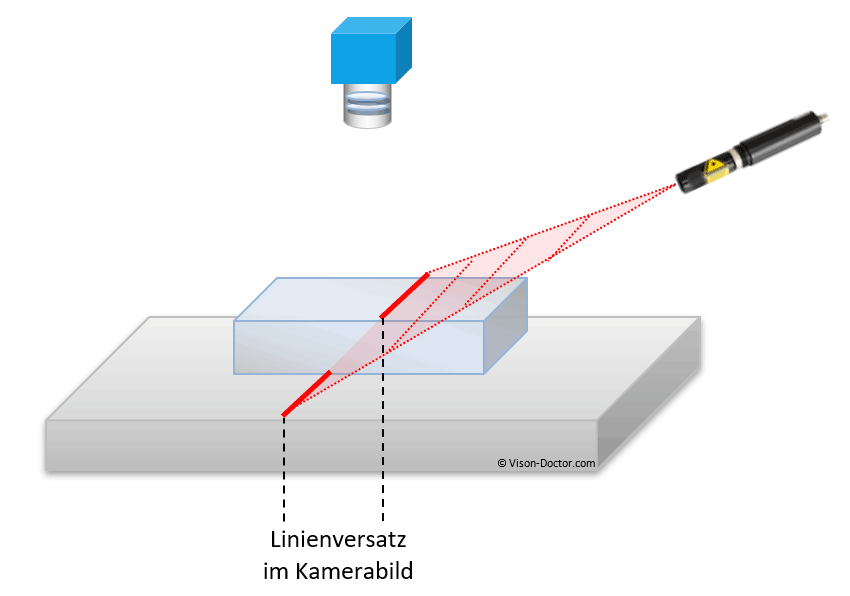
\includegraphics[width=0.6\linewidth]{img/grundlagen/lasertriangulation_2}
		\caption{Positionen bei der Lasertriangulation}
		\captionsource{Abbildung entnommen aus \citep{noauthor_prinzip_nodate}}
		\label{fig:lasertriangulation_position}
	\end{figure}
	
	Die Entwicklung lässt sich in zwei Abschnitte aufteilen. Der erste Abschritt ist die Erarbeitung des Lasertriangulationssensors. Dessen Aufgabe ist es, eine aufgenommene Laserlinie in eine korrekte Punktewolke umzusetzen. Danach muss es dem Sensor ermöglicht werden, sich über das Objekt zu bewegen. Möglich ist auch, dass Objekt unter dem Sensor durch zu bewegen. \newline
	Wichtig ist, dass die Kamera und Laser in einem Winkel zueinander über dem Objekt angebracht sind (Abb. (\ref{fig:lasertriangulation}), (\ref{fig:lasertriangulation_position})). Dabei ist ausschlaggebend, dass Kamera und Laser fest angebracht sind und sich zueinander nicht bewegen. Nur der ganze Sensor ist bewegbar, dabei bleiben dann Kamera und Laser zueinander in der gleichen Position.
	\label{chap:grundlegender_aufbau}
	
	\subsection{Pinhole Camera Model}
	Wenn eine Kamera ein Bild aufnimmt, ist das eine Abbildung eines dreidimensionalen Raumes (die Szene) auf eine zweidimensionale Ebene (das Bild). Der Lasertriangulationssensor soll diesen Prozess umgekehrt realisieren. Die Grundlage ist das aufgenommene Bild. Ein Bild besteht aus Pixeln. Ausgehend von diesem, soll der dreidimensionale Raum digital abgebildet werden. Das bedeutet, dass für jeden Pixel eine definierte Abbildung im dreidimensionalen Raum gefunden werden muss. Für diese Abbildungen ist in OpenCv das \textbf{Pinhole Camera Model} implementiert. Hier wird die Kamera digital als eine Lochkamera begriffen. \newline
	\begin{figure}[h]
		\centering
		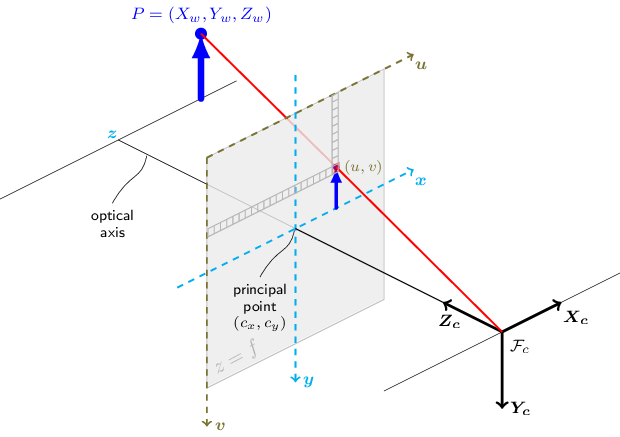
\includegraphics[width=0.7\linewidth]{img/grundlagen/pinhole_camera_model.png}
		\caption{Pinhole Camera Model}
		\captionsource{Abbildung entnommen aus \citep{noauthor_opencv_nodate-2}}
		\label{fig:pinhole-camera-model}
	\end{figure}
	In Abb. (\ref{fig:pinhole-camera-model}) ist dieses Modell dargestellt. An dem optischen Zentrum orientiert sich das Kamera-Koordinatensystem (\( F_c \)). Dabei wäre das optisches Zentrum bei einer Lochkamera die Lochblende oder bei einer herkömmlichen Kamera der optische Sensor. Wenn mit einer Lochkamera ein Bild aufgenommen wird, erscheint die Abbildung auf dem Kopf gespiegelt auf einer Bildebene. Das hat physikalische Gründe. Das Pinhole Kamera Model ist aber rein digital. So muss die Bildebene nicht hinter dem optischen Sensor sein. Sie wird zwischen dem optischen Zentrum und der Abbildung im dreidimensionalen Raum dargestellt. So kann ein Punkt in der Szene als Vektor begriffen werden, der durch die Bild-Ebene einen Pixel definiert und zum optischen Zentrum führt \citep[vgl.][]{dawson-howe_simple_1994}. Zu sehen in Abb. (\ref{fig:pinhole-camera-model}) als die rote Linie. In diesem Fall ist das Bild und die genaue Position eines Pixels mit u und v bekannt. Das Ziel ist es, die dazugehörige 3D-Koordinate (P) zu erhalten.
	\newpage 
	
	\subsection{Mathematische Grundlage}
	Die Grundlage für die Berechnungen mit den Pixeln aus einem Bild ist die folgende Formel:
	
	\begin{equation}
	s \; p_{pix} = A \begin{bmatrix} R|t \end{bmatrix} p_w
	\label{eq:basic_trans}
	\end{equation}
	
	Sie beschreibt die Projektion eines 3D-Punktes in eine Szene zu einem Punkt in der Bild-Ebene. Hierbei ist \( p_{pix} \) der Pixel im Bild. \( p_w \) ist die Welt-Koordinate, welche gesucht wird. \( A \) ist die Kamera-Matrix.\( \begin{bmatrix} R|t \end{bmatrix} \) ist eine Rotation und Translation und beschreibt eine Transformation vom Kamerakoordinatensystem zum Weltkoordinatensystem. Die genaue Entstehung der Formel beschreibt OpenCv in \citep[vgl.][]{noauthor_opencv_nodate-2}. Kamera-Matrix, Rotation und Translation sind hierbei neu. Die genaue Bedeutung wird in dem Kapitel \ref{chap:kalibierung} Kalibrierung genannt. Zum Verstehen der Formel ist hier nur wichtig, dass diese durch eine Kamerakalibrierung herausgefunden werden können \citep[vgl.][]{dawson-howe_simple_1994}. Die Variablen sind also bekannt. Kamera-Matrix und Rotation sind beide jeweils 3x3 Matrizen. Die Translation wird durch einen Vektor (3x1) beschrieben. 
	
	\begin{equation}
	s \; \begin{bmatrix}
	u \\ 
	v \\ 
	1
	\end{bmatrix} = \begin{bmatrix}
	f_x & 0 & c_x \\
	0 & f_y & c_y \\
	0 & 0 & 1
	\end{bmatrix} \times \begin{bmatrix}
	r_{11} & r_{12} & r_{13} & t_1 \\ 
	r_{21} & r_{22} & r_{23} & t_2 \\ 
	r_{31} & r_{32} & r_{33} & t_3
	\end{bmatrix} \times \begin{bmatrix}
	X \\ 
	Y \\ 
	Z \\
	1
	\end{bmatrix}
	\label{eq:basic_trans_complete}
	\end{equation}
	
	In der Formel (\ref{eq:basic_trans_complete}) wird dies noch einmal genauer gezeigt. Bekannt sind also \( p \), \( A \) und \( \begin{bmatrix} R|t \end{bmatrix} \). Unbekannte Variablen sind \( s \) der Scale-Factor und \( p_w \) die Weltkoordinate.
	
	\subsubsection{Koordinaten-Transformationen}
	Um den 3D-Punkt im Weltkoordinatensystem anhand eines Pixels zu errechnen, wird die grundlegende Formel umgestellt. Die folgende Abbildung (\ref{fig:pinhole-camera-model_transformations}) zeigt nochmal das Pinhole Camera Model und verdeutlicht dabei die angewandten Transformationen.
	
	\begin{figure}[h]
		\centering
		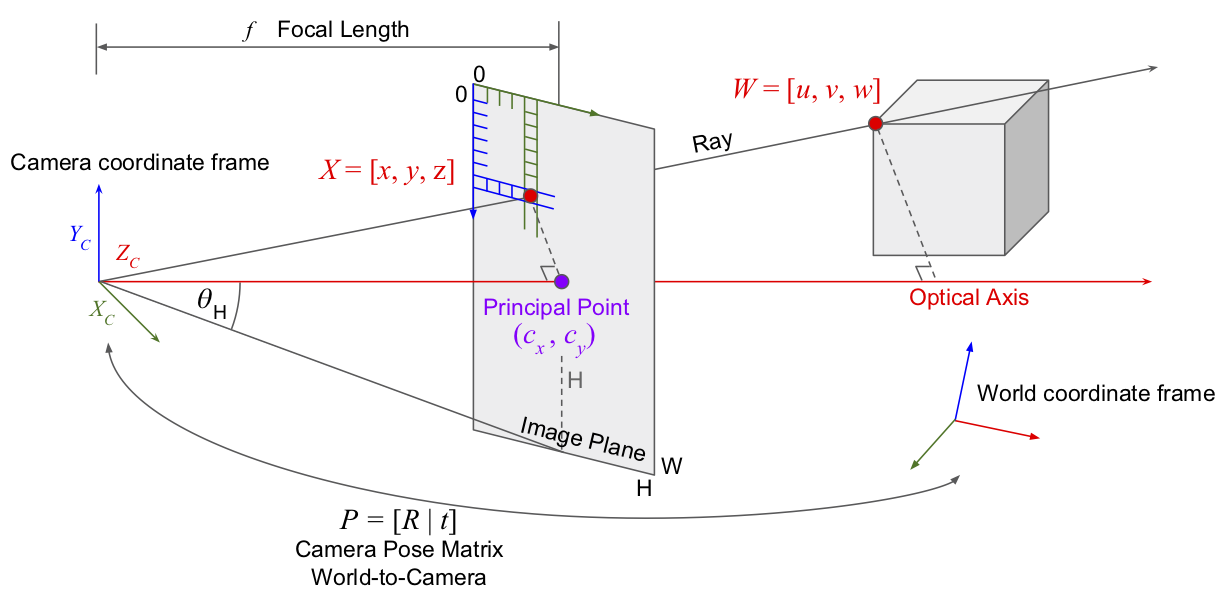
\includegraphics[width=0.9\linewidth]{img/grundlagen/pinhole_camera_model_2.png}
		\caption[Transformationen]{Transformationen im Pinhole Camera Model}
		\captionsource{Abbildung entnommen aus \citep{pinhole_camera_model}}
		\label{fig:pinhole-camera-model_transformations}
	\end{figure}
	
	Das Ziel ist es, den 3D-Punkt (in Abb. (\ref{fig:pinhole-camera-model_transformations}) \( W \)) im Weltkoordinatensystem zu errechnen. Die Rotation (R) und Translation (t) werden für die Umrechnung in das Kamerakoordinatensystem benötigt. Das sind die sogenannten extrinsischen Parameter. In Abb. (\ref{fig:pinhole-camera-model_transformations}) wird diese Transformation unter \( P \) der \textbf{Camera Pose Matrix} dargestellt. \newline
	Die Kamera-Matrix beschreibt die Transformation zur Bild-Ebene bzw. den Pixelkoordinatensystem. Die Matrix enthält die sogenannten intrinsischen Parameter. Das ist die in Abb. (\ref{fig:pinhole-camera-model_transformations}) gezeigte \textbf{Focal Length} \( f \), welche den Abstand vom Kamera-Koordinatensystem zur Bild-Ebene beschreibt. Hinzu kommt der \textbf{Principal Point}. Dieser befindet sich in dem Zentrum der Bild-Ebene. Beides zusammen ergibt die gezeigte Matrix aus (\ref{eq:basic_trans_complete}) \citep[vgl.][]{noauthor_opencv_nodate-1}. Letztendlich wird damit die Umrechnung vom Kamerakoordinatensystem (in Abb. (\ref{fig:pinhole-camera-model_transformations}) \textbf{Camera coordinate frame}) zur Bild-Ebene (in Abb. (\ref{fig:pinhole-camera-model_transformations}) \textbf{Image Plane}) dargestellt. \newline 
	Es ist möglich, einen Pixel im Bild auszuwählen und mithilfe dieser Parameter den entsprechenden Punkt im Weltkoordinatensystem errechnen. Dazu muss die Formel (\ref{eq:basic_trans}) nach dem Punkt im Weltkoordinatensystem umgestellt werden.
	
	\begin{equation}
	\begin{aligned}
	\begin{bmatrix} A \end{bmatrix} \begin{bmatrix} R|t \end{bmatrix} p_w &= s \; p_{pix} \\
	\begin{bmatrix} R|t \end{bmatrix} p_w &= s \begin{bmatrix} A \end{bmatrix}^{-1} p_{pix} \\
	\begin{bmatrix} R \end{bmatrix} p_w &= s \begin{bmatrix} A \end{bmatrix}^{-1} p_{pix} - t \\
	p_w &= s \begin{bmatrix} R \end{bmatrix}^{-1} \begin{bmatrix} A \end{bmatrix}^{-1} p_{pix} - \begin{bmatrix} R \end{bmatrix}^{-1} t \\
	p_w &= s \; \vec{a} - \vec{b} \\
	wobei: \quad \vec{a} & = \begin{bmatrix} R \end{bmatrix}^{-1} \begin{bmatrix} A \end{bmatrix}^{-1} p_{pix} \\
	\vec{b} &= \begin{bmatrix} R \end{bmatrix}^{-1} t
	\end{aligned}
	\label{eq:pixel_zu_welt}
	\end{equation}
	
	Diese Gleichung ist die Grundlage der Errechnung von 3D-Informationen. \( \vec{a} \) und \( \vec{b} \) dienen zur Vereinfachung. Wenn \( \begin{bmatrix} R \end{bmatrix} \), \( \begin{bmatrix} A \end{bmatrix}^{-1} \) und \( p_{pix} \) miteinander verrechnet werden entsteht ein Vektor (\( \vec{a} \)). Genauso entsteht aus\( \begin{bmatrix} R \end{bmatrix}^{-1} \) und \( t \) der Vektor (\( \vec{b} \)). Zusätzlich beschreibt \( s \; \vec{a} - \vec{b} \) eine Gleichung für eine Linie im dreidimensionalen Raum. Damit stellt sie den beschriebenen Vektor in \citep[vgl.][S. 3]{dawson-howe_simple_1994} und die rote Linie in Abb. (\ref{fig:pinhole-camera-model}) und (\ref{fig:pinhole-camera-model_transformations}) dar. \newline
	Der neue Ausgangspunkt ist die errechnete Weltkoordinate. Nach Aufgabenstellung sollen errechnete Koordinaten immer aus Sicht der Kamera dargestellt werden. Dazu wird die folgende Transformation benötigt. 
	
	Weltkoordinate zu Kamerakoordinate:
	\begin{equation}
	p_{cam} = \begin{bmatrix} R \end{bmatrix} \; p_{welt} + t
	\label{eq:welt_zu_kamera}
	\end{equation}
	
	Kamerakoordinate zur Weltkoordinate:
	\begin{equation}
	p_{welt} = \begin{bmatrix} R \end{bmatrix}^{-1} \; (p_{cam} - t)
	\label{eq:kamera_zu_welt}
	\end{equation}
	
	Anzumerken ist noch, dass \( s \) der Scale-Factor immer noch eine Unbekannte ist. Es scheint also, als ob die Gleichung (\ref{eq:pixel_zu_welt}) noch nicht lösbar sei. Sobald konkrete Werte ausgerechnet werden sollen, muss \( s \) bekannt sein. Das passiert zum ersten Mal beim Erstellen der Ebenengleichung für die Laser-Ebene bei der extrinsischen Kalibrierung. Dabei wird auch darauf eingegangen, wie \( s \) errechnet werden kann.  
	
	\newpage
	
	\label{chap:transformationen}
	\subsection{Bildverarbeitung}
	Bekannt sind nun gewisse Grundlagen, wie mit einem ausgewählten Pixel im Bild umgegangen werden kann. Die Rechnungen und Transformationen sollen aber nicht auf zufällige oder sogar alle Pixel im Bild angewandt werden. Sie sollen auf ganz bestimmte ausgewählte Pixel erfolgen. Und zwar ganz genau diese, die zur abgebildeten Laserlinie gehören. Die Laserlinie ist immer unser Ausgangspunkt für die 3D-Informationen. Alle anderen Pixel interessieren im Grunde nicht. \newline
	Pixel können einfach und eindeutig als Tupel benannt werden. Sie können als Punkt in einem zweidimensionalen Koordinatensystem begriffen und dann mit einem horizontalen und vertikalen Wert genau gekennzeichnet werden. Benötigte wird eine Menge an diesen Tupeln, für die gilt, dass sie Teil der Laserlinie im Bild sind. Mit diversen Methoden der Bildverarbeitung können diese Pixel herausgefunden und abgespeichert werden, um mit ihnen weiterarbeiten zu können. Das folgende Kapitel bildet somit einen Algorithmus ab, dessen Ziel es ist, ein Bild entgegenzunehmen und die Pixel der Laserlinie zurückzugeben. 
	
	\label{chap:bildverarbeitung}
	\subsubsection{Das Erkennen der Laserlinie}
	Der erste Schritt des Algorithmus muss sein, die Laserlinie im Bild zu erkennen. Ein wichtiges Kriterium dabei ist die Genauigkeit der ausgewählten Pixel. Jeder Pixel, der vom Algorithmus markiert wird, aber nicht zur eigentlichen Laserlinie gehört, wird in einem Fehler in der am Ende erstellten Punktewolke enden. Es wird also ein Punkt im Raum gezeigt, der nicht zur eingescannten Oberfläche passt. Dieser hängt dann beispielsweise in der Luft bzw. ist an einer Stelle im Koordinatensystem, wo sich eigentlich nichts befindet. Dieses sogenannte Rauschen soll möglichst gering sein. \newline
	Im Zuge einer umfangreichen Recherche zum Thema Lasertriangulation und OpenSource-Produzierten Laserlinienscannern wurde ein Paper von Bajpai und Perelman \citep[vgl.][]{baj-per}, die auch einen Laserlinienscanner entwickelt haben, als Grundlage gewählt. Nicht nur bei dem Finden der Laserlinie, auch in diversen anderen Schritten der Errechnung von 3D-Punkten aus den Laserlinien-Pixeln ist dieses Paper eine Grundlage und Hilfestellung. Gemäß der dort verwendeten Methodik wurde die Idee übernommen, zwei Bilder aufzunehmen. In einem ist der Laser angeschaltet, in dem anderen nicht. Wenn diese Bilder voneinander abgezogen werden, kommen im Grunde genau die Veränderungen hervor. Da sich nichts anderes im Bild verändern sollte, außer das Erscheinen der Laserlinie, wird diese genau aufgezeigt.
	Voraussetzung dafür ist, dass die Umgebung der zu scannenden Fläche gleich bleibt. Einwirkungen wären zum Beispiel Änderungen bei den Lichtverhältnissen bzw. bei der Beleuchtung oder auch eine Bewegung von Objekten zwischen der Aufnahme der zwei Bilder. Solche Einwirkungen würden in ungewolltem Rauschen enden oder sogar die Laserlinie falsch positionieren. Weitere Informationen hierzu befinden sich ebenfalls im Kapitel \ref{chap:probleme_schwierigkeiten} Probleme und Schwierigkeiten. Diese Anforderungen werden für den zu entwickelnden Laserlinien-Scanner akzeptiert. Ebenfalls sind es Anforderungen, die nicht direkt von der Software beeinflusst werden können. Sie sollten somit beim Aufbau des Scanners genauer beachtet werden und auf die Bildverarbeitung keinen Einfluss mehr haben dürfen. Die Methode ist außerdem ohne Probleme über OpenCv umsetzbar.
	
	\begin{figure}[h]
		\centering
		\subfloat[]{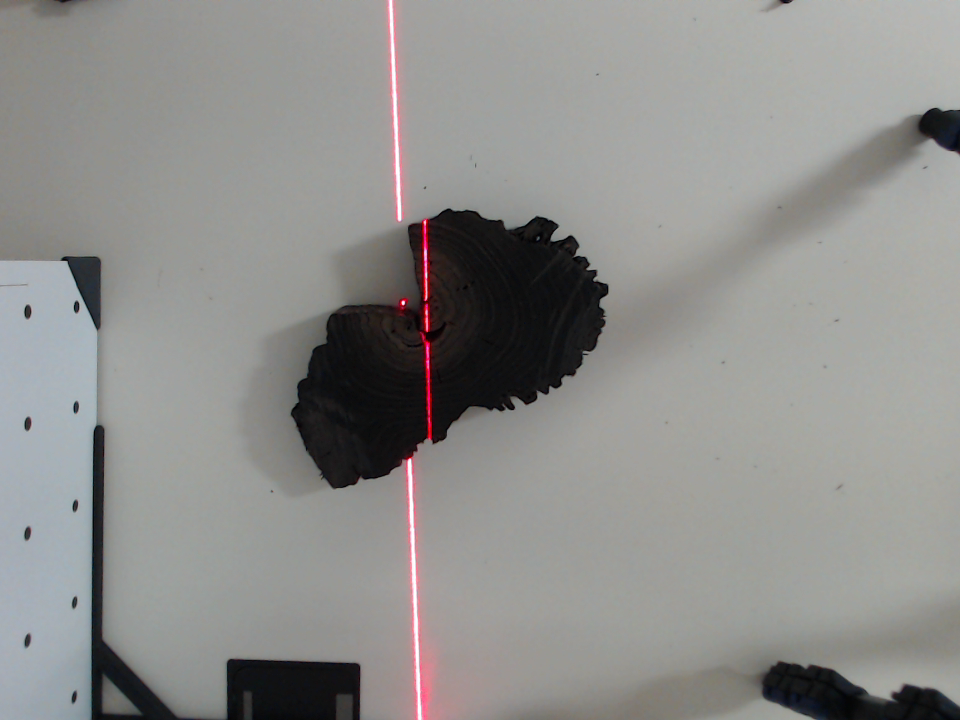
\includegraphics[width=0.325\linewidth]{img/hauptteil/bildverarbeitung/surface_img_1.png} \label{subfig:surface_laser}}
		\subfloat[]{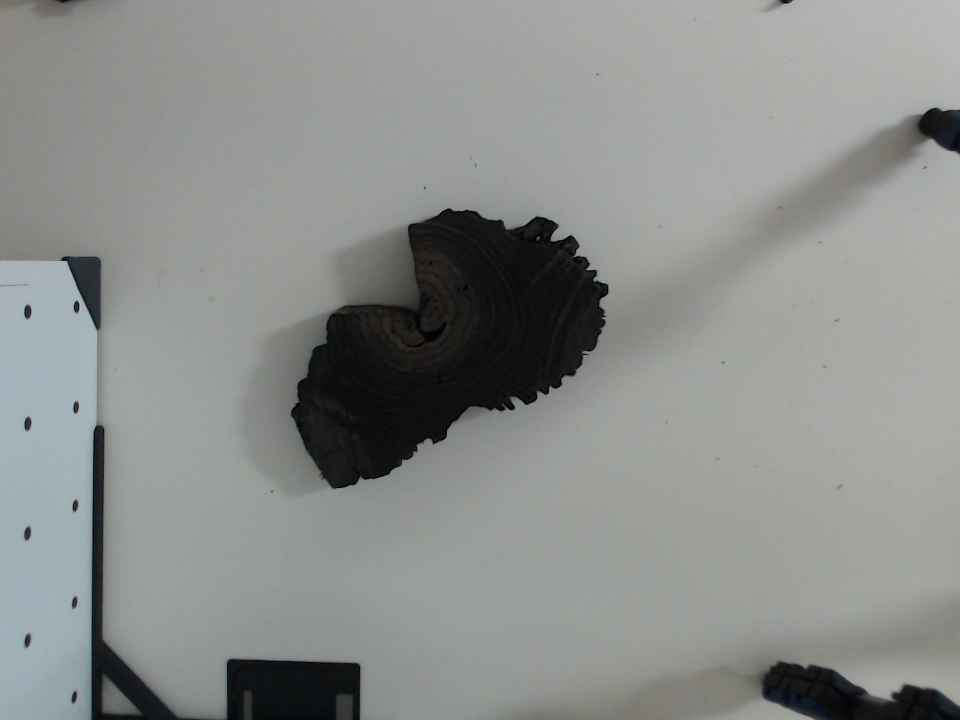
\includegraphics[width=0.325\linewidth]{img/hauptteil/bildverarbeitung/surface_img_0.png} \label{subfig:surface}}
		\subfloat[]{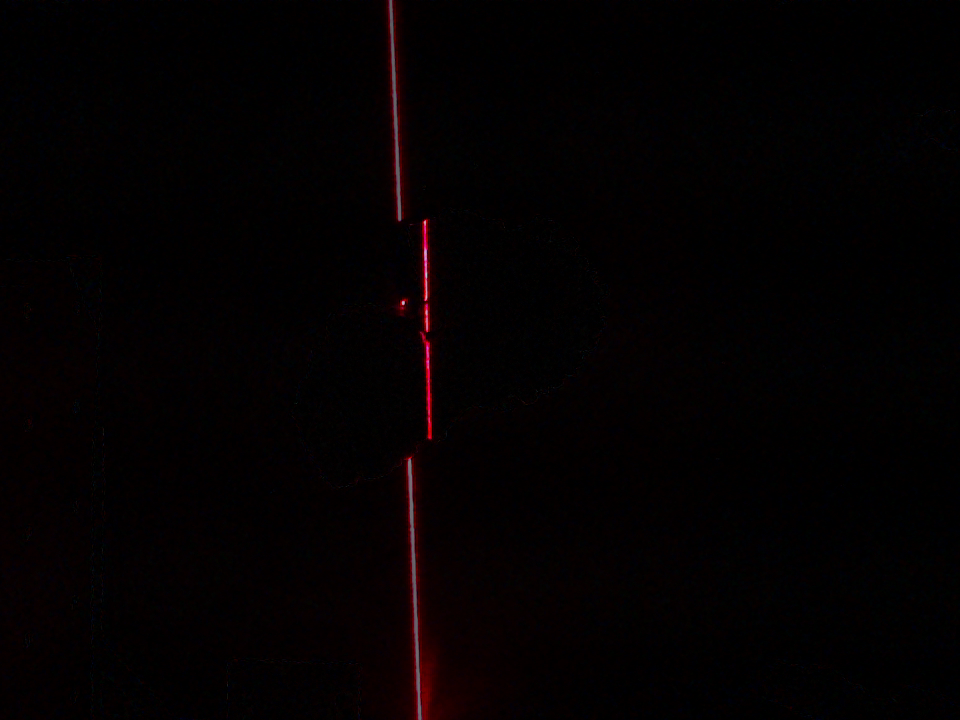
\includegraphics[width=0.325\linewidth]{img/hauptteil/bildverarbeitung/surface_diff.png} \label{subfig:surface_diff}}
		\caption{Subtraktion der Bilder}
		\label{fig:sub_imgs}
	\end{figure} 
	
	Festzuhalten ist damit, dass die Kamera zwei Bilder aufnehmen muss, eins Bild mit Laserlinie und ein Bild ohne. Das Bild ohne Laserlinie (\ref{subfig:surface}) wird dann von dem mit Laserlinie (\ref{subfig:surface_laser}) abgezogen. Der Algorithmus zum Finden der Laserlinien-Pixel arbeitet dann mit der Differenz (\ref{subfig:surface_diff}).
	
	\newpage
	
	\subsubsection{Umwandlung zu einem Grauwert-Bild}
	Für einen Menschen ist die Laserlinie jetzt schon auf einem Blick gut erkennbar. Ein Algorithmus braucht allerdings spezifische Informationen, um die Pixel auszuwählen. Auch die Pixel, die nicht eindeutig zur Laserlinie gehören sind nicht komplett schwarz mit einem RGB-Wert von (R=0, G=0, B=0). Einen kleinen für den Menschen zumeist nicht sichtbaren Unterschied in zwei nacheinander aufgenommenen Bildern wird es immer geben. 
	
	\begin{figure}[h]
		\centering
		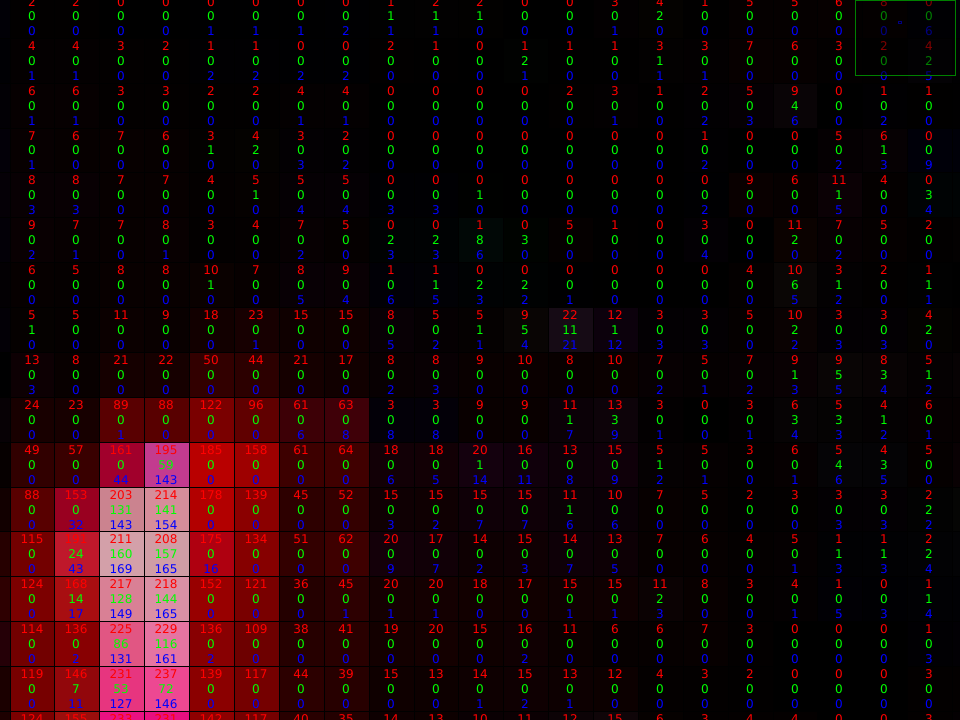
\includegraphics[width=0.75\linewidth]{img/hauptteil/bildverarbeitung/pixel_values.png}
		\caption[Pixel-Werte der Laserlinie]{Pixel-Werte in einem Ausschnitt aus \ref{subfig:surface_diff} am Rand der Laserlinie}
		\label{fig:pix_values}
	\end{figure} 
	
	Die Abbildung zeigt gut die Pixel der Laserlinie unten links. Die verschiedenen Farbbereiche sind stark vertreten, vor allem der Rote. Die Pixel, die kein Teil der Laserlinie sind, besitzen nur sehr schwache Werte in den drei Farbbereichen. Nach einer Regelung muss hier immer noch genau festgelegt werden, welche Pixel für die Laserlinie ausgewählt werden. Die Differenz von den zwei Bildern macht dies allerdings einfacher. Gleichbleibende Stellen zwischen den beiden Bildern wie zum Beispiel sehr helle Stellen oder auch andere rote Stellen sind in dem Differenz-Bild nicht mehr erkennbar. Ohne diesen Schritt wären diese womöglich nicht genau von der Laserlinie zu unterscheiden. \newline
	Als zweiter Schritt wird das Bild zu einem Grauwert-Bild konvertiert. Vorteil davon ist, dass nicht mehr der RGB-Wert mit drei eigenen Werten ausschlaggebend ist, sondern nur noch die Intensität, bzw. der Grauwert eines Pixels. Die jeweilige Intensität für einen Pixel berechnet OpenCv nach der folgenden Formel \cite[Vgl.][]{noauthor_opencv_nodate}:
	\begin{equation}
	Y = 0.299 \cdot R + 0.587 \cdot G + 0.114 \cdot B
	\label{eq:rgb_to_grey}
	\end{equation}
	Die Formel (\ref{eq:rgb_to_grey}) zeigt, dass aus den drei Farbwerten nun ein einzelner Grauwert errechnet wird. Allgemein kann dabei festhalten werden, dass je höher die einzelnen Farbinformationen waren, um so höher wird auch der Grauwert bzw. die Intensität sein. Das betrifft die Pixel der Laserlinie. Die anderen Pixel besitzen sehr geringe Farbwerte und werden deshalb auch eine geringe Intensität aufweisen. 
	
	\begin{figure}[h]
		\centering
		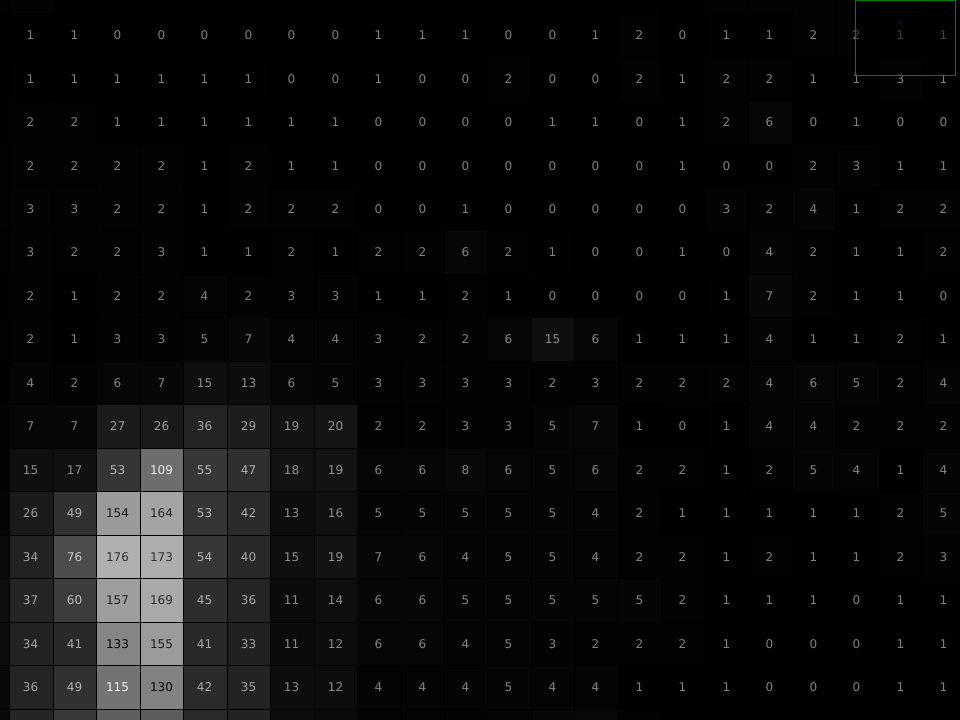
\includegraphics[width=0.75\linewidth]{img/hauptteil/bildverarbeitung/pixel_values_gray.png}
		\caption[Pixel-Werte im Grauwertbild]{Der selbe Ausschnitt wie in Abb. (\ref{fig:pix_values}), nur als Grauwertbild konvertiert.}
		\label{fig:pix_values_gray}
	\end{figure} 
	
	Die Abbildungen (\ref{fig:pix_values}) und (\ref{fig:pix_values_gray}) zeigen auch, dass eine Laserlinie bis zu 4 oder 5 Pixel breit sein kann. Für die Weiterverarbeitung soll sie allerdings nur eine Breite von einem Pixel haben. Dazu wird in jeder Pixel-Zeile in einem Bild nach der höchsten Intensität gesucht. Das ist jedoch nur sinnvoll, wenn die Laserlinie im Bild von oben nach unten geht. Der Laser muss demnach entsprechend zur Kamera angebracht werden. Diese Anforderung kann schon im Aufbau des Sensors beachtet werden. Im Kapitel \ref{chap:grundlegender_aufbau} wurde beschrieben, dass Kamera und Laser zueinander in der gleichen Position bleiben. Demnach kann der Laser entsprechend so angebracht werden, dass er im Kamerabild entsprechend aufgenommen wird.
	
	\subsubsection{Gauß-Filter}
	Die einfachste Methode wäre also jede Zeile nach der höchsten Intensität zu suchen und den betreffenden Pixel auszuwählen. Dieser Pixel befindet sich je nach Aufnahme jedoch nicht genau in der Mitte der Laserlinie. Die erarbeiteten Linien können so sehr \glqq wellig\grqq{} werden, da Pixel untereinander zum Teil stark in ihrer Position in der Zeile abweichen. Den Pixel mit der höchsten Intensität als Ausgangspunkt zu nehmen ist gut, jedoch sollen die umliegenden Pixel einen Einfluss machen können, um die Genauigkeit der Laserlinie zu erhöhen. Dazu wurden zwei Vorgänge entwickelt. \newline
	Die erste Methode ist es, einen Gauß-Filter über das Grauwert-Bild zu legen. Ein Gauß-Filter ist ein Weichzeichner, der umgangssprachlich ein Bild verwischt oder unscharf macht bzw. das Grauwertbild glättet \citep[vgl.][S. 134ff]{nischwitz_bildverarbeitung_2020}. Der Gauß-Filter wird auf jeden Pixel im Bild angewandt. Dabei ändert er den Wert des ausgewählten Pixels in Abhängigkeit der umliegenden Pixel. In diesem Projekt wird er dabei in einer Reichweite von einem 5x5-Feld definiert. Das bedeutet, dass ausgehend von dem ausgewählten Pixel ein 5x5-Feld betrachtet wird. Der Gauß-Filter ist ein Tiefpassfilter und wirkt damit möglichem Rauschen im Bild entgegen. Wenn ein einzelner Pixel ein hohen Wert aufweist, jedoch alle anderen um diesen herum im Vergleich niedriger sind, wird der Pixel-Wert nach der Filter-Operation niedriger ausfallen. So werden demnach vereinzelte Pixel mit hoher Intensität dunkler gemacht. Bei Gruppen von Pixeln werden die Intensitäten aneinander angepasst.
	
	\subsubsection{Das Erstellen von Subpixeln}
	Nachdem der Filter verwendet wurde, kommt die Operation, in der jede Zeile des Bildes nach dem Laserlinien-Pixel abgesucht wird. Hier wird zuerst der Pixel mit der höchsten Intensität gesucht. Dabei kann immer noch mehr  Genauigkeit erzielt werden, wenn man die Pixel links und recht neben dem Ausgewählten mit beachtet. So fließt nicht nur die Intensität als Auswahlkriterium ein, sondern auch die benachbarten Pixel der Laserlinie in dieser Zeile. Da die erschlossenen Pixel in 3D-Koordinaten umgewandelt werden und somit vom Bild und der Pixel-Darstellung getrennt werden, ist es nicht mehr notwendig nur ganze Zahlen zu verwenden. Die Werte können also auch Nachkommastellen haben und sogenannte Subpixel ergeben. Für dieses Errechnen des passenden Subpixel wurde ein Algorithmus erstellt, der wie folgt funktioniert:
	
	$\underline{1. \; Grenzwert}$
	
	Zuerst wird ein passender Grenzwert für die Intensität gesucht, um eine Grenze festzulegen, ab welchen Wert überhaupt ein Pixel gefunden werden soll. Wenn die maximale Intensität in einer Zeile unter dem gewählten Grenzwert liegt, wird diese übersprungen. Damit wird auch ungewolltes Rauschen entfernt, da eine Intensität, die so niedrig ist, nicht zur Laserlinie gehören kann. Ein im Vorhinein festgelegter Grenzwert ist dabei nicht ausreichend, da dieser nicht an das aktuelle Bild angepasst wäre. Bilder können unterschiedlich ausfallen und nicht wie gewollt auf den Grenzwert reagieren. So können zu viele oder zu wenig Zeilen übersprungen werden. Der Grenzwert soll genau auf das aktuelle Bild angepasst sein. Die Otsu-Methode ist ein Schwellenwertverfahren, welches genau den gewollten Wert liefern kann \citep[vgl.][]{otsu_tresh}. Dabei wird von einem Grauwertbild ein Histogramm erstellt. Dieses wird analysiert und ein passender individueller Grenzwert ausgegeben. Die höchste Intensität der aktuellen Zeile wird auf diesen geprüft. Wenn sie zu niedrig ist, ist auch die ganze Zeile zu dunkel und wird nicht als Teil der Laserlinie angesehen.
	
	$\underline{2. \; Einbeziehen \; der \; benachbarten \; Pixel}$
	
	Der Ausgangspunkt ist jetzt der Pixel mit der höchsten Intensität und dieser liegt über dem errechneten Grenzwert. Die benachbarten Pixel sollen jetzt in einen endgültigen Wert mit einbezogen werden. Um das zu erreichen, wird eine Parabel genutzt. Es gilt eine quadratische Funktion in der Form \( ax^2 + bx + c = I_x \), wobei \( I \) die Intensität und \( x \) die Position in der jeweiligen Zeile ist. Bei einem Bild, das beispielsweise 1920 Pixel breit ist, ist das ein Wert zwischen 0 und 1919. Die quadratische Funktion wird auf den ausgewählten Pixel und seine Nachbarn angewandt. Somit gilt:
	
	\begin{equation}
	\begin{aligned}
	ax^2 + bx + c &= I_x \\
	a(x+1)^2 + b(x+1) + c &= I_{x+1} \\
	a(x-1)^2 + b(x-1) + c &= I_{x-1} \\
	daraus \; folgt: \\
	\underbrace{\begin{pmatrix}
		x^2 & x & 1 \\
		(x+1)^2 & (x+1) & 1 \\
		(x-1)^2 & (x-1) & 1 
		\end{pmatrix}}_{\substack{X}} \underbrace{ \begin{pmatrix}
		a \\
		b \\
		c
		\end{pmatrix}}_{\substack{\vec{abc}}} &= \begin{pmatrix}
	I_x \\
	I_{x+1} \\
	I_{x-1}
	\end{pmatrix}
	\end{aligned}
	\label{eq:subpixel_x}
	\end{equation}
	
	Das Ziel ist es den Vektor \( \vec{abc} \) herauszufinden. Da die Intensitäten und die x-Werte bekannt sind, ist \( \vec{abc} \) die einzige Unbekannte und kann errechnet werden. Im nächsten Schritt soll das Maximum der Parabel herausgefunden werden. Sie befindet sich dort, wo die tatsächliche Intensität am höchsten ist. Dieser x-Wert befindet sich dann in den meisten Fällen zwischen zwei Pixeln. Um das Maximum zu finden wird die Nullstelle der Ableitung errechnet. Dafür gilt:
	
	\begin{equation}
	\begin{aligned}
	2a \cdot x + b &= 0 \\
	x &= \frac{-b}{2a}
	\end{aligned}
	\end{equation}
	
	\( b \) und \( a \) sind durch das Errechnen von \( \vec{abc} \) bekannt und ein Wert für \( x \) kann gefunden werden.
	
	In der Rechnung fällt auf, dass x für jede Zeile individuell ausgerechnet wird. Dabei ändert sich in (\ref{eq:subpixel_x}) die Werte für \( x \) und die Intensitäten. Hier kann man die Berechnung vereinfachen. Wählt man für \( x = 0\), entsteht die folgende Matrix:
	
	\begin{equation}
	X = \begin{pmatrix}
	0 & 0 & 1 \\
	1 & 1 & 1 \\
	1 & -1 & 1
	\end{pmatrix}
	\end{equation}
	
	Wenn \( \vec{abc} \) mit dieser Matrix und den individuellen Intensitäten berechnet wird, erhält man die Abweichung zu Mitte. Dabei ist die Mitte 0 und das entspricht dem ausgewählten Pixel mit der höchsten Intensität. Man errechnet eine Zahl zwischen -1 und 1. Diese wird mit der x-Position des Ausgangspixel in der Zeile verrechnet. Der Algorithmus wurde somit vereinfacht, da sich in jeder Rechnung nur der Intensitäten-Vektor ändert und immer die gleiche Matrix \( X \) gewählt werden kann.
	
	\begin{figure}[h]
		\centering
		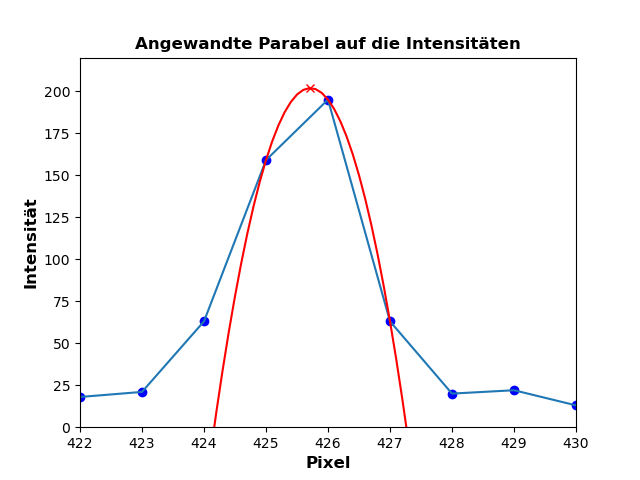
\includegraphics[width=0.7\linewidth]{img/hauptteil/bildverarbeitung/parable_intensities.png}
		\caption[Parabel für die Intensitäten]{Parabel für die Intensitäten. Die Blauen Punkte kennzeichnen einen Pixel und seine jeweilige Intensität. Die Parabel wird durch den Punkt mit der höchsten Intensität und seine Nachbarn gelegt.}
		\captionsource{Der gezeigte Ausschnitt stammt aus einer ausgewählten Zeile in Abb. (\ref{subfig:surface_diff})}
		\label{fig:parable}
	\end{figure} 
	
	Mit dem Finden des x-Wert ist die Bearbeitung einer Zeile fertig. Es gibt nun eine eindeutige 2D-Koordinate für einen Punkt der Laserlinie. Der Algorithmus geht über jede Zeile (y) und findet einen x-Wert. Dabei fügt er die gefundenen Subpixel (x, y) in einer Liste zusammen. Die Menge dieser Subpixel ist die Abbildung der Laserlinie in einen 2-dimensionalen Raum (Abb. (\ref{fig:pix_koord})). Diese wurde als Output gefordert.
	
	\begin{figure}[h]
		\centering
		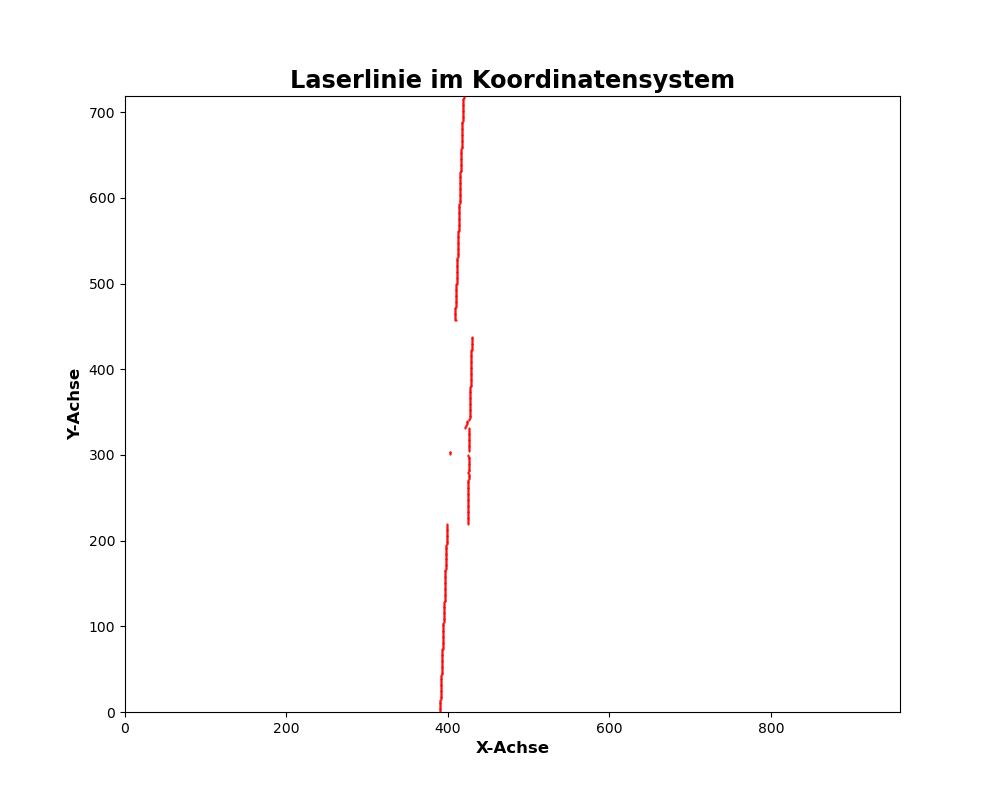
\includegraphics[width=0.8\linewidth]{img/hauptteil/bildverarbeitung/pixel_koord.png}
		\caption[Subpixel im Koordinatensystem]{Die Subpixel können nun in einem Koordinatensystem dargestellt werden.}
		\label{fig:pix_koord}
	\end{figure} 

	Wenn man die Abb. (\ref{fig:pix_koord}) und (\ref{subfig:surface_diff}) vergleicht, fällt auf, dass die Abbildung im Koordinatensystem gespiegelt ist. Das liegt daran, dass die Nummerierung der Pixel im Bild oben links beginnt (der Nullpunkt mit Pixel (0, 0)) und bei einem Koordinatensystem unten links. 

	\label{chap:erkennen_der_laserlinie}

\clearpage

% ----------------------------------------------------------------------------------------------------------
% Hauptteil
% ----------------------------------------------------------------------------------------------------------
% ----------------------------------------------------------------------------------------------------------
% Eigene Projektbeschreibung und -ergebnisse
% ----------------------------------------------------------------------------------------------------------
\section{Hauptteil - Projektbeschreibung und Projektergebnisse}\label{ergebnisse}
	\subsection{Kalibrierung}
		Die Kamerakalibrierung ist ausschlaggebend, um die Formel (\ref{eq:basic_trans_complete}) benutzen zu können. Durch sie wird die Kamera-, Rotationsmatrix und der Translationsvektor gefunden. Dabei unterscheidet man zwischen intrinsische und extrinsischer Kalibrierung, bei denen auch ein unterschiedliches Kalibrierverfahren angewandt wird.
		
		\label{chap:kalibierung}
		\subsubsection{Intrinsische Kalibrierung}
		Die intrinsische Kalibrierung beschäftigt sich mit dem \textit{Inneren} der Kamera. Ergebnis der Kalibrierung ist die Kameramatrix \( A \). Die Kamerakalibrierung ist in OpenCv implementiert und wurde in diesem Projekt genutzt [OpenCv-CamCalib]. Die Implementierung richtet sich nach der Kamerakalibrierung nach Zhang [Zhang] und nach Bouguet [Bouguet]. \newline
		Der grundlegende Vorgang ist es, ein bekanntes Muster in verschiedenen Positionen mit der Kamera aufzunehmen. So ein Muster ist beispielsweise ein Schachbrett, welches auch in dieser Arbeit für das Kalibrieren benutzt wurde. Die Maßen von den Kacheln sind dementsprechend dann bekannt und der Druck muss genau sein. Dabei muss es sich nicht um ein herkömmliches Schachbrett handeln. Die Größe und die Menge an Kachel kann zum kalibrieren angegeben werden. Man muss OpenCv also sagen, nach welchem Schachbrett der Algorithmus suchen muss.
		
		\begin{figure}[h]
			\centering
			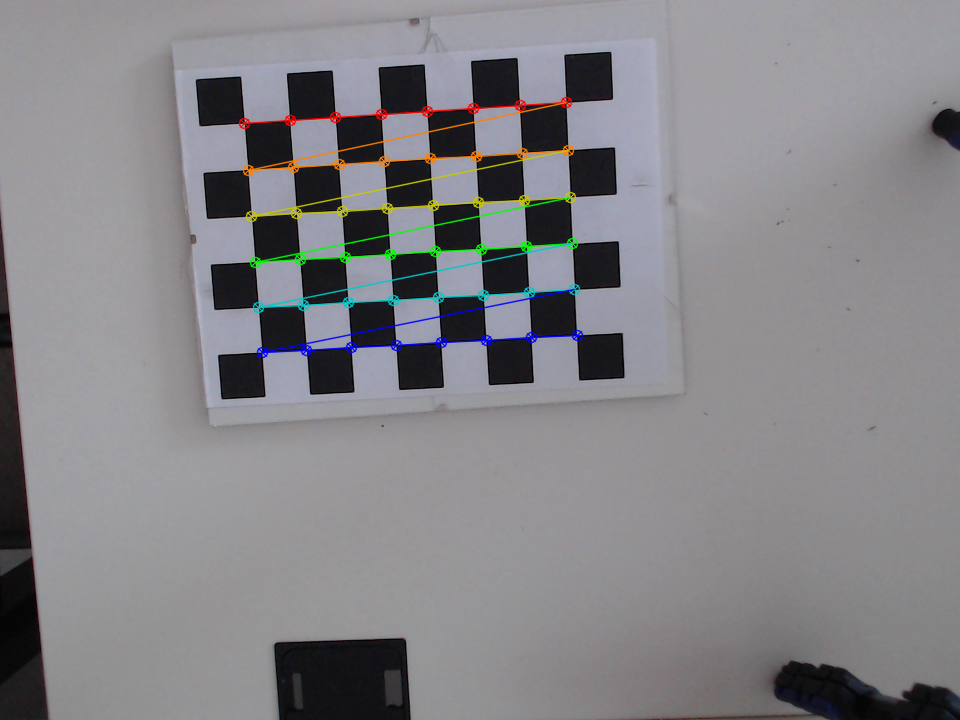
\includegraphics[width=0.32\linewidth]{img/hauptteil/calibration/chessboard_corner_0.png}
			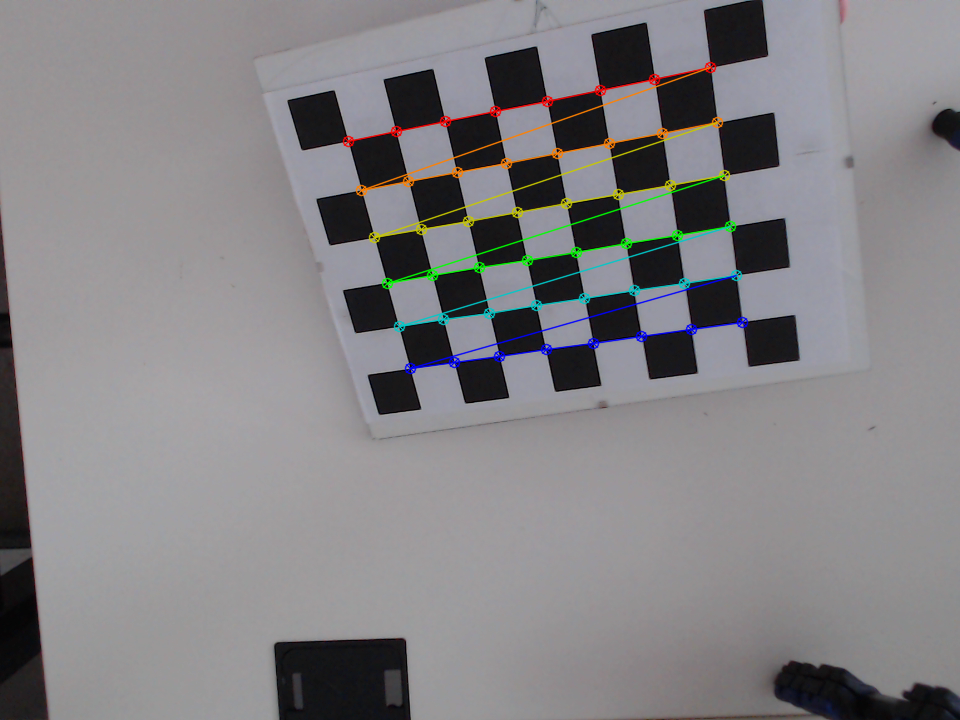
\includegraphics[width=0.32\linewidth]{img/hauptteil/calibration/chessboard_corner_1.png}
			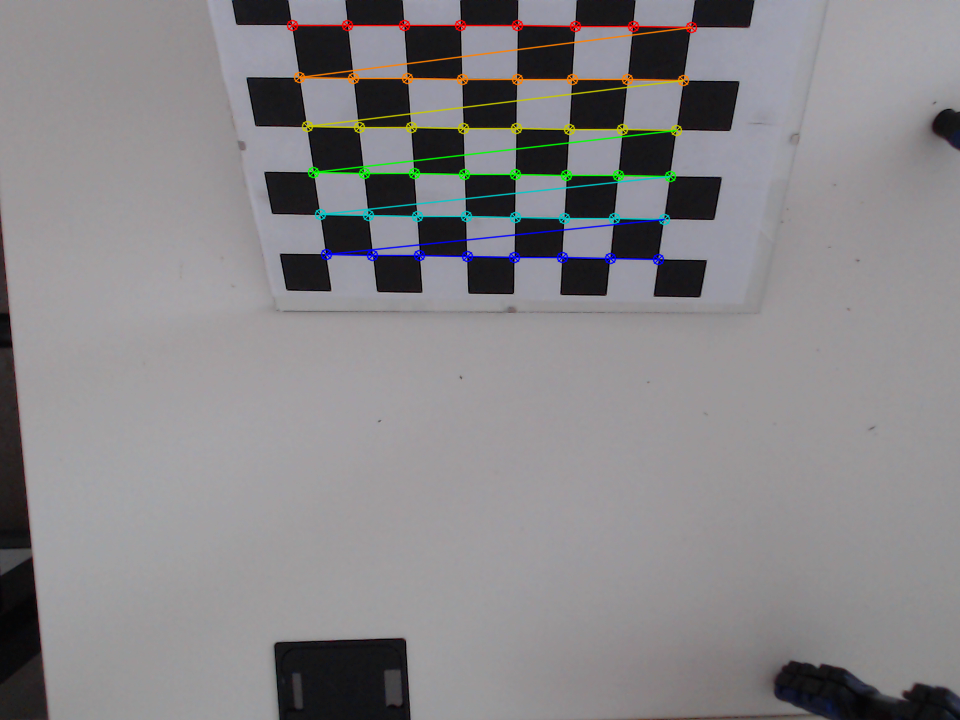
\includegraphics[width=0.32\linewidth]{img/hauptteil/calibration/chessboard_corner_2.png}
			%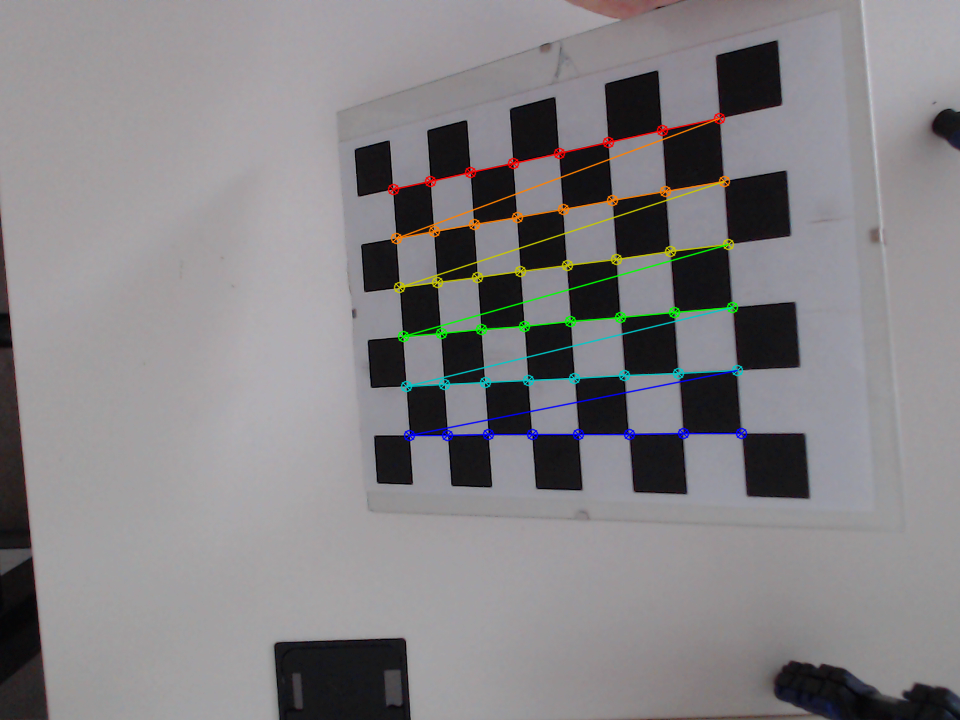
\includegraphics[width=0.39\linewidth]{img/hauptteil/calibration/chessboard_corner_3.png}
			\caption[Schachbrett-Kalibrierung]{Schachbrett-Kalibrierung mit dem Schachbrett aus verschieden Positionen}
			\label{fig:chessboards}
		\end{figure}
	
		Die benutzte Methode heißt \textbf{calibrateCamera()}. Sie nimmt beliebig viele Bilder entgegen. In der eigenen Implementierung wurde gemäß [OpenCv-Cam] vorgegangen. Dabei handelt es sich um die offizielle Einführung zur Kamerakalibrierung von OpenCv.In dem Beispiel in Abb.: (\ref{fig:chessboards}) wurden der Einführung folgend auch die Ecken des definierten Schachbrettes eingezeichnet. Damit kann man im Grunde sichbar machen, dass der Algorithmus das Schachbrett richtig erkannt hat. Gemäß [OpenCv-Cam] werden mindestens 10 Bilder benötigt, um gute Ergebnisse zu liefern. Daran wurde sich ebenfalls gehalten. Die Methode gibt die folgenden Werte zurück:
		
		$\underline{Kameramatrix}$
		
		Die \textbf{Kameramatrix} wird errechnet und ausgegeben. Dabei handelt es sich um die vollwertige Matrix \( A \) aus den Formeln (\ref{eq:basic_trans}) und (\ref{eq:basic_trans_complete}).
		
		$\underline{Distortion-Koeffizienten}$
		
		Die Distortion-Koeffizienten werden gemäß [OpenCv-Cam] geliefert. Distortion bedeutet Verzerrung und bezieht sich auf das aufgenommene Bild. Dies Auswirkungen sind, dass aufgenommene gerade Linien in der Szene im Bild nicht mehr gerade dargestellt werden. Sie biegen sich bzw. sind verzerrt. Es gibt zwei verschiedene Verzerrungen, beschrieben in [Dist] und von OpenCv selbst in [OpenCv-CamCalib].
		
		\begin{figure}[h]
			\centering
			\subfloat[]{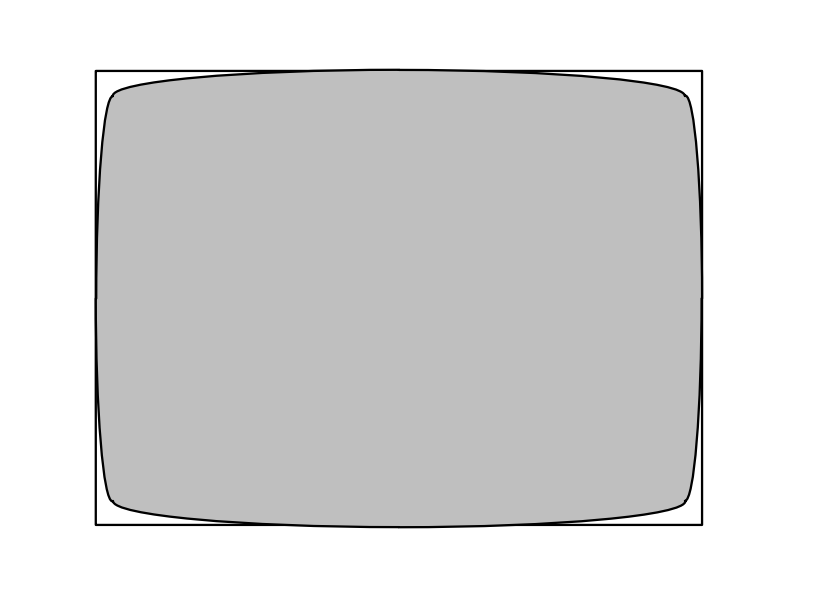
\includegraphics[width=0.4\linewidth]{img/hauptteil/calibration/barrel_dist.png} 	\label{subfig:barrel_dist}} 
			\subfloat[]{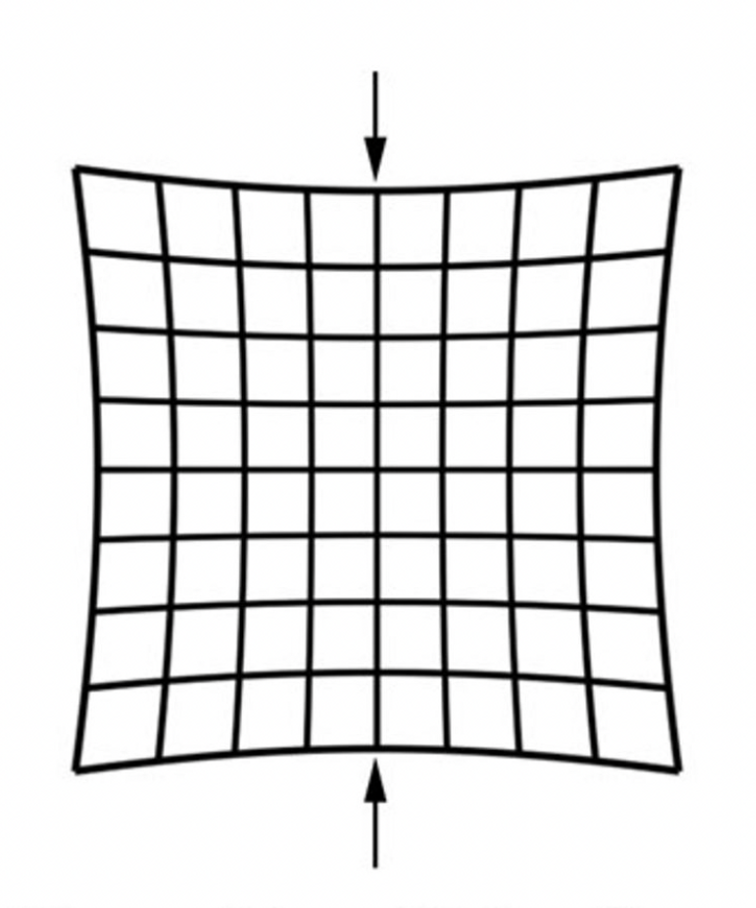
\includegraphics[width=0.4\linewidth]{img/hauptteil/calibration/pinc_dist.png}
				\label{subfig:pinc_dist}}
			\caption[Verzerrung bei Bildern]{Verzerrung bei Bildern; \ref{subfig:barrel_dist} zeigt die Tonnen-Verzerrung (engl.: Barrel-Distortion) und \ref{subfig:pinc_dist} die Kissen-Verzerrung (engl.: Pincushion-Distortion)}
			\captionsource{https://www.learningwithexperts.com/photography/blog/look-out-for-lens-distortion}
			\label{fig:distortion}
		\end{figure}
	
		Um dieser Verzerrung entgegenzuwirken gibt es in OpenCv die Methode \textbf{undistort()}. Diese bringt ein Bild wieder in den normalen Zustand und benutzt dabei die gefunden Koeffizienten [OpenCv-Cam]. Das benutzen dieser Methode ist unumgänglich. Die Laserlinie ist bei einem ebenen Untergrund gerade. Wenn diese allerdings gebogen ist, führt das beim Aufspannen auf die Ebene zu Höhenunterschieden zwischen den Punkten. Die Verzerrung ist nicht Teil des Pinhole Camera Models und somit auch kein Teil der Formel (\ref{eq:basic_trans}). Bevor mit aufgenommenen Bildern gearbeitet wird, werden die jedoch mit der Methode \textbf{undistort()} entzerrt.
		
		\begin{figure}[h]
			\centering
			\subfloat[]{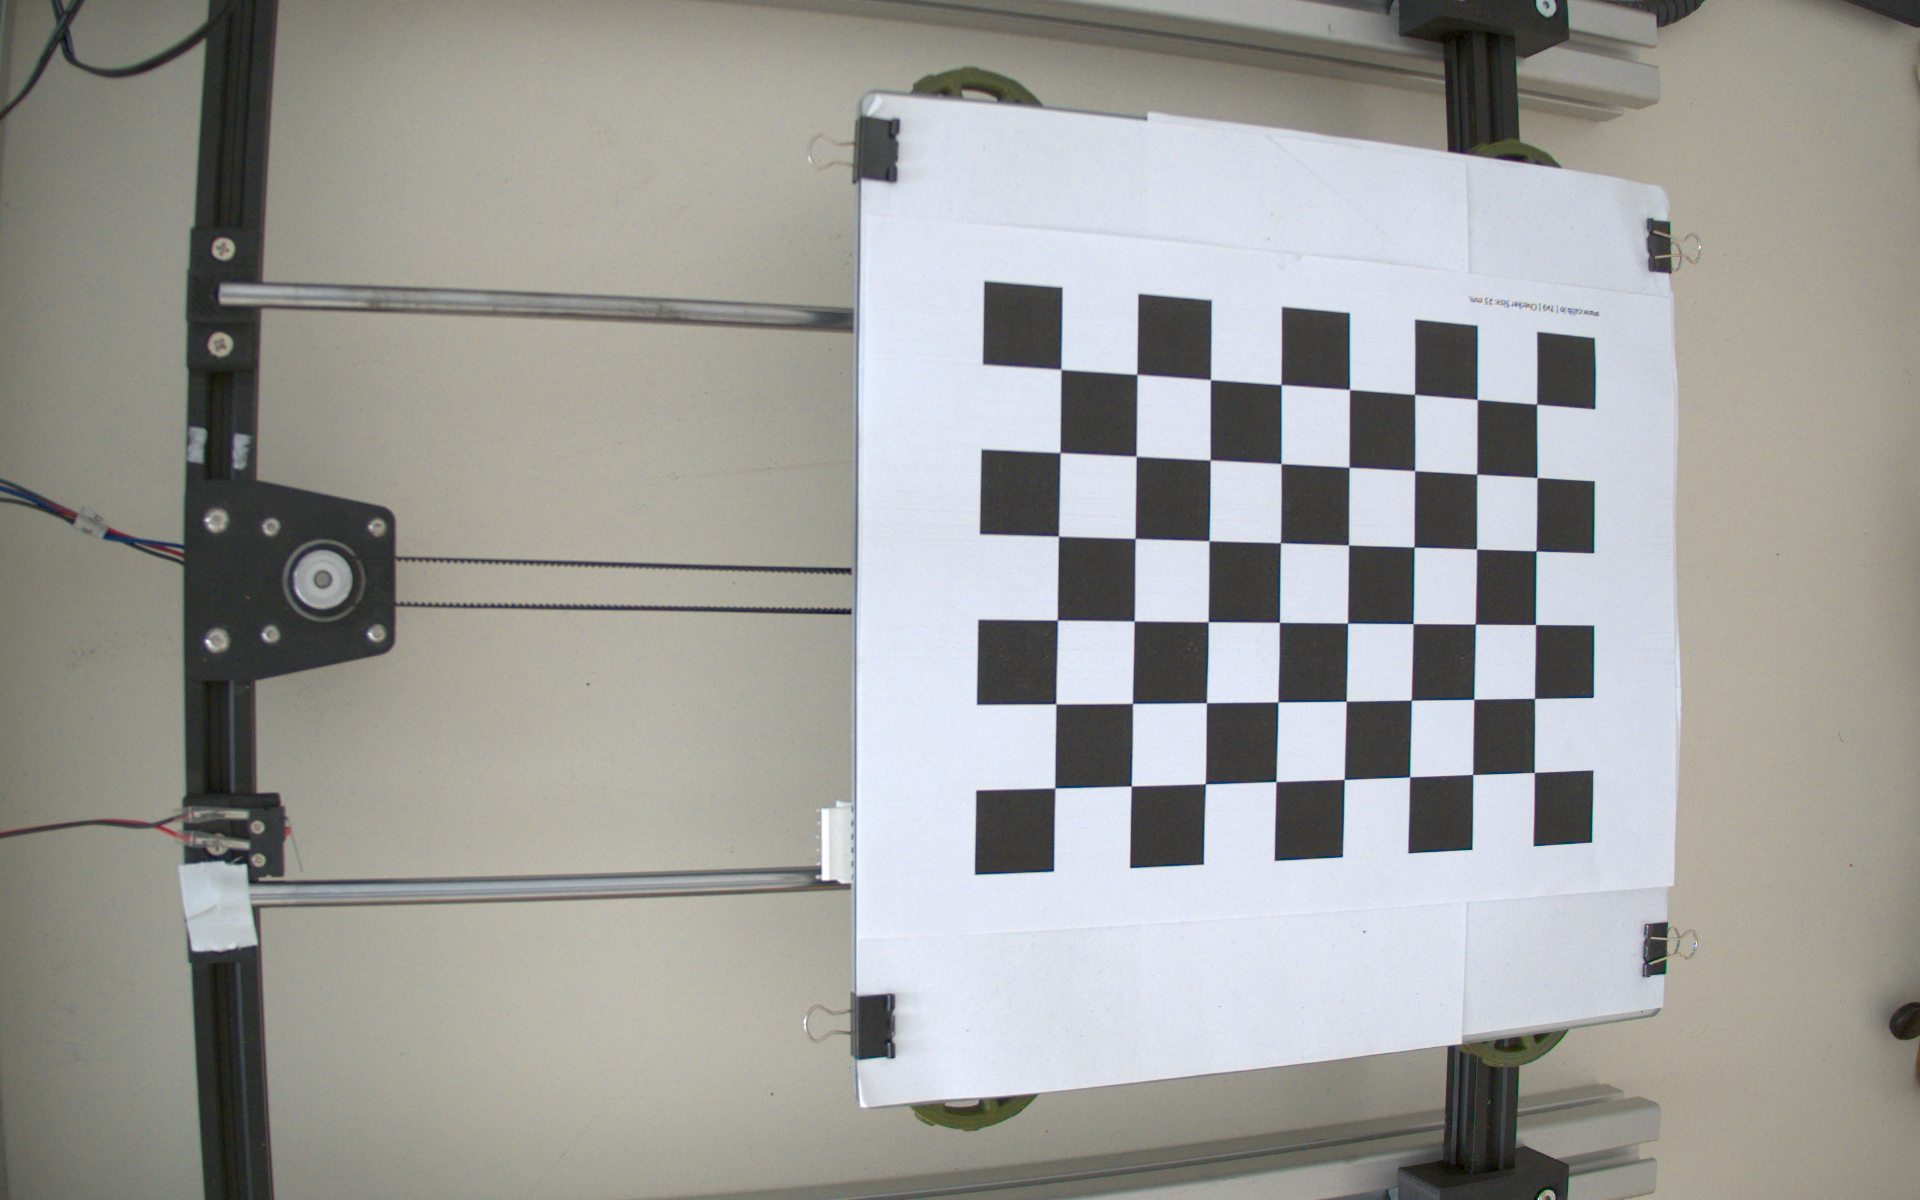
\includegraphics[width=0.49\linewidth]{img/hauptteil/calibration/distorted.png} 	\label{subfig:distorted}} 
			\subfloat[]{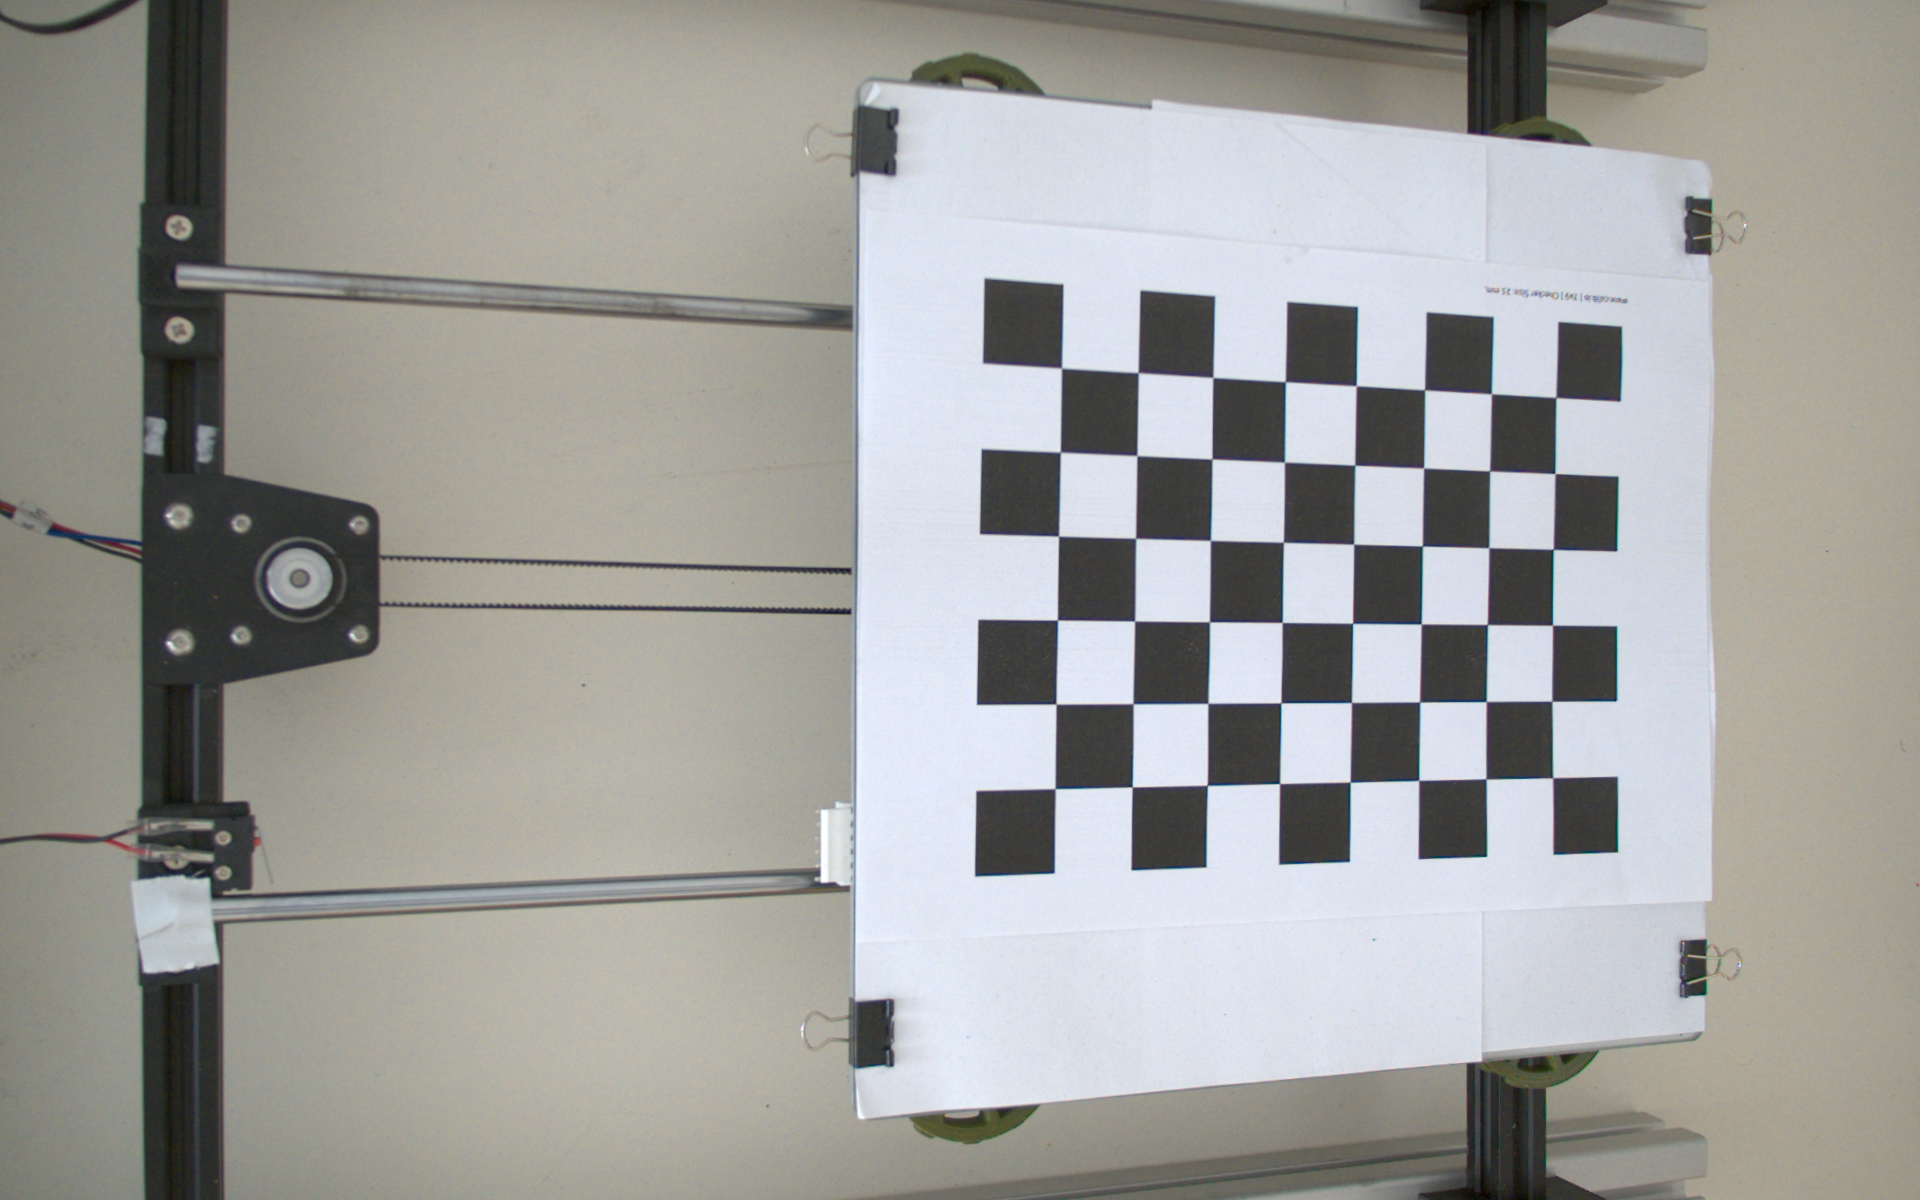
\includegraphics[width=0.49\linewidth]{img/hauptteil/calibration/undistorted.png}
				\label{subfig:undistorted}}
			\caption[Beispiel für die Verzerrung in Bildern]{Hier ein direktes Beispiel aus dem Aufbau. \ref{subfig:distorted} zeigt das Bild vor dem Anwenden von \textbf{undistort()} und \ref{subfig:undistorted} danach.}
			\label{fig:distortion_bsp}
		\end{figure}
	
		Ebenso ist erkennbar, dass es sich bei den verwendeten Kameramodell um eine \textit{Barrel-Distortion} (siehe Abbildung \ref{subfig:barrel_dist}) handelt.
		
		$\underline{Rotationen \; und \; Translationen}$
		
		Die Methode gibt ebenfalls eine Rotationsmatrix und einen Translationsvektor für jedes übergebene Schachbrett zurück. Das sind extrinsische Parameter. In jedes Schachbrett wird ein Koordinatensystem gelegt. Die Rotation und Translation beschreiben dann die Transformation von der Kamera zu diesem Koordinatensystem. Es werden also auch schon extrinsische Parameter geliefert. Diese sind allerdings für den Lasertriangulationssensor selbst nicht ausschlaggebend. Damit dieser mit dem Laser kalibriert werden kann, also eine Ebenen-Gleichung für den Laser gefunden wird, muss der Laser mit auf den Bildern abgebildet sein. Dann kann man die Linie in Bezug auf das gefundene Weltkoordinatensystem weiterverwenden. Für die extrinsische Kalibrierung wurde eine extra Methode entwickelt, welche im nächsten Kapitel beschrieben wird. Die Rotation und Translation zu den verschiedenen Positionen des Schachbrettes sind nicht von Interesse. 
		
		Die intrinsische Kalibrierung ist nur dazu da, die Kameramatrix zu finden und die Distortion-Koeffizienten zu bestimmen, damit die verwendeten Bilder nicht verzerrt sind. Die Kameramatrix ist explizit für die Kamera gültig, mit welcher das Schachbrettmuster aufgenommen wurde. Sie kann also bestimmt werden und ist dann für alle folgenden Rechnungen gültig und unverändert. Genauso verhält es sich mit den Distortion-Koeffizienten. Das bedeutet, dann der Lasertriangulationssensor initial einmal mit dieser Methode kalibriert werden muss, um die intrinsischen Parameter zu bestimmen. Danach werden die Kameramatrix und die Distortion-Koeffizienten abgespeichert und die extrinsische Kalibrierung kann beginnen. 
			\label{chap:kalibrierung_intrinsisch}
			
		\newpage
		\subsubsection{Extrinsische Kalibrierung}
		Die extrinsische Kalibrierung beschäftigt sich allgemein damit die Kamera zu den eingebauten Linienlaser zu kalibrieren. Genauer gesagt geht es nicht konkret um den Laser, sondern die Laserlinie. Ziel dabei ist es, eine Ebenengleichung zu erhalten, die sich im Kamerakoordinatensystem befindet den Laser repräsentiert. Um sich das besser vorzustellen, kann nochmal Abb.: (\ref{fig:lasertriangulation}) eingesehen werden. Hier ist die symbolische Ebene des Lasers rot markiert. Die dazugehörige Gleichung beschreibt dann die Position des Laserlinienstrahls. Grundlegend richtet sich die Methode, um die Ebenen-Gleichung zu finden erneut nach Bajpai und Perelman [baj-per]. \newline
		Bekannt ist, dass durch eine Kamerakalibrierung die Rotation und Translation herausgefunden werden können. Durch die intrinsische Kalibrierung ist die Kameramatrix bekannt. Dabei wurde ein Schachbrett aus verschiedenen Positionen aufgenommen. Ziel ist es nun ein Schachbrett mit einer Laserlinie aufzunehmen. Die allgemeine Transformationsformel (\ref{eq:basic_trans_complete}) kann gelöst werden. Mit dem im Kapitel \ref{chap:bildverarbeitung} vorgestellten Verfahren werden die Pixel, die die Laserlinie abbilden gefunden. Nur diese werden in die Formel (\ref{eq:basic_trans_complete}) eingesetzt. Dabei können jetzt die 3D-Punkte errechnet werden, welche sich in dem Weltkoordinatensystem befinden. Das Weltkoordinatensystem liegt dabei auf dem Schachbrett und ist durch die Rotationsmatrix und den Translationsvektor bestimmt. Aus einer Linie kann jedoch keine Ebene abgeleitet werden. Was ist aber, wenn sich im selben Bild ein zweites Schachbrett befindet, welches nicht eben, sondern in einem gewissen Winkel zu dem ersten befindet. Das zweite Schachbrett hat dabei dann ein eigenes Weltkoordinatensystem. Da jedoch alle Transformationen bekannt sind, ist es möglich die Laserlinien-Punkte des einen Koordinatensystem in das andere zu transformieren. Betrachtet werden nun zwei Laserlinien, die in einem Winkel zueinander in einem einheitlichen Koordinatensystem stehen. Mit dieser Ausgangslage ist es möglich eine Ebene in die Punkte zu legen. Dabei gibt es diverse Möglichkeiten eine Ebene an Punkte zu fitten und alle liefern eine Ebenengleichung. Rein logisch sind sogar nur mindestens drei Punkte notwendig, um in einem dreidimensionalen Raum eine Ebene zu beschreiben. In diesem Fall sind es weitaus mehr Punkte, die zum finden der Ebene berücksichtigt werden können. \newline
		In [baj-per] wird dann bei jedem Durchgang, bei dem eine Laserlinie in eine Punktewolke übersetzt wird, eine aktuelle neue Ebenengleichung erstellt und die Oberflächenpunkte errechnet. Die Ausgangslage ist hier jedoch etwas anders. Die Idee ist es nach der intrinsischen Kalibrierung eine einmalige extrinsische Kalibrierung vorzunehmen. Es wurde schon erwähnt, dass sich Kamera und Laser in ihrer Position zueinander nicht verändern. Damit bleibt auch die Ebenen-Gleichung in Bezug zur Kamera immer gleich. Die einmal  gefundene Ebenengleichung ist also allgemeingültig für den folgenden Scann. Dieser Vorgang der extrinsischen Kalibrierung soll hier nochmal genau beschrieben werden.
		
		$\underline{Zwei \; Schachbretter \; in \; einem \; Bild}$
		
		Um die extrinsische Kalibrierung auszuführen soll also ein Bild von zwei Schachbrettern gemacht werden. Dabei ist es nötig, das sie in einem Winkel zueinander stehen. Das hat den Grund, dass die verschiedenen Laserlinien einen Winkel bilden müssen, um darin eine Ebene zu finden. Der Winkel ist dabei grundsätzlich egal. Jedoch sollte kein zu hoher oder zu niedriger Winkel gewählt werden, damit dieser nicht zu eng bzw. zu flach ausfällt. Zu diesem Zweck wurde eine eigene Unterlage designt.
		
		\begin{figure}[h]
			\centering
			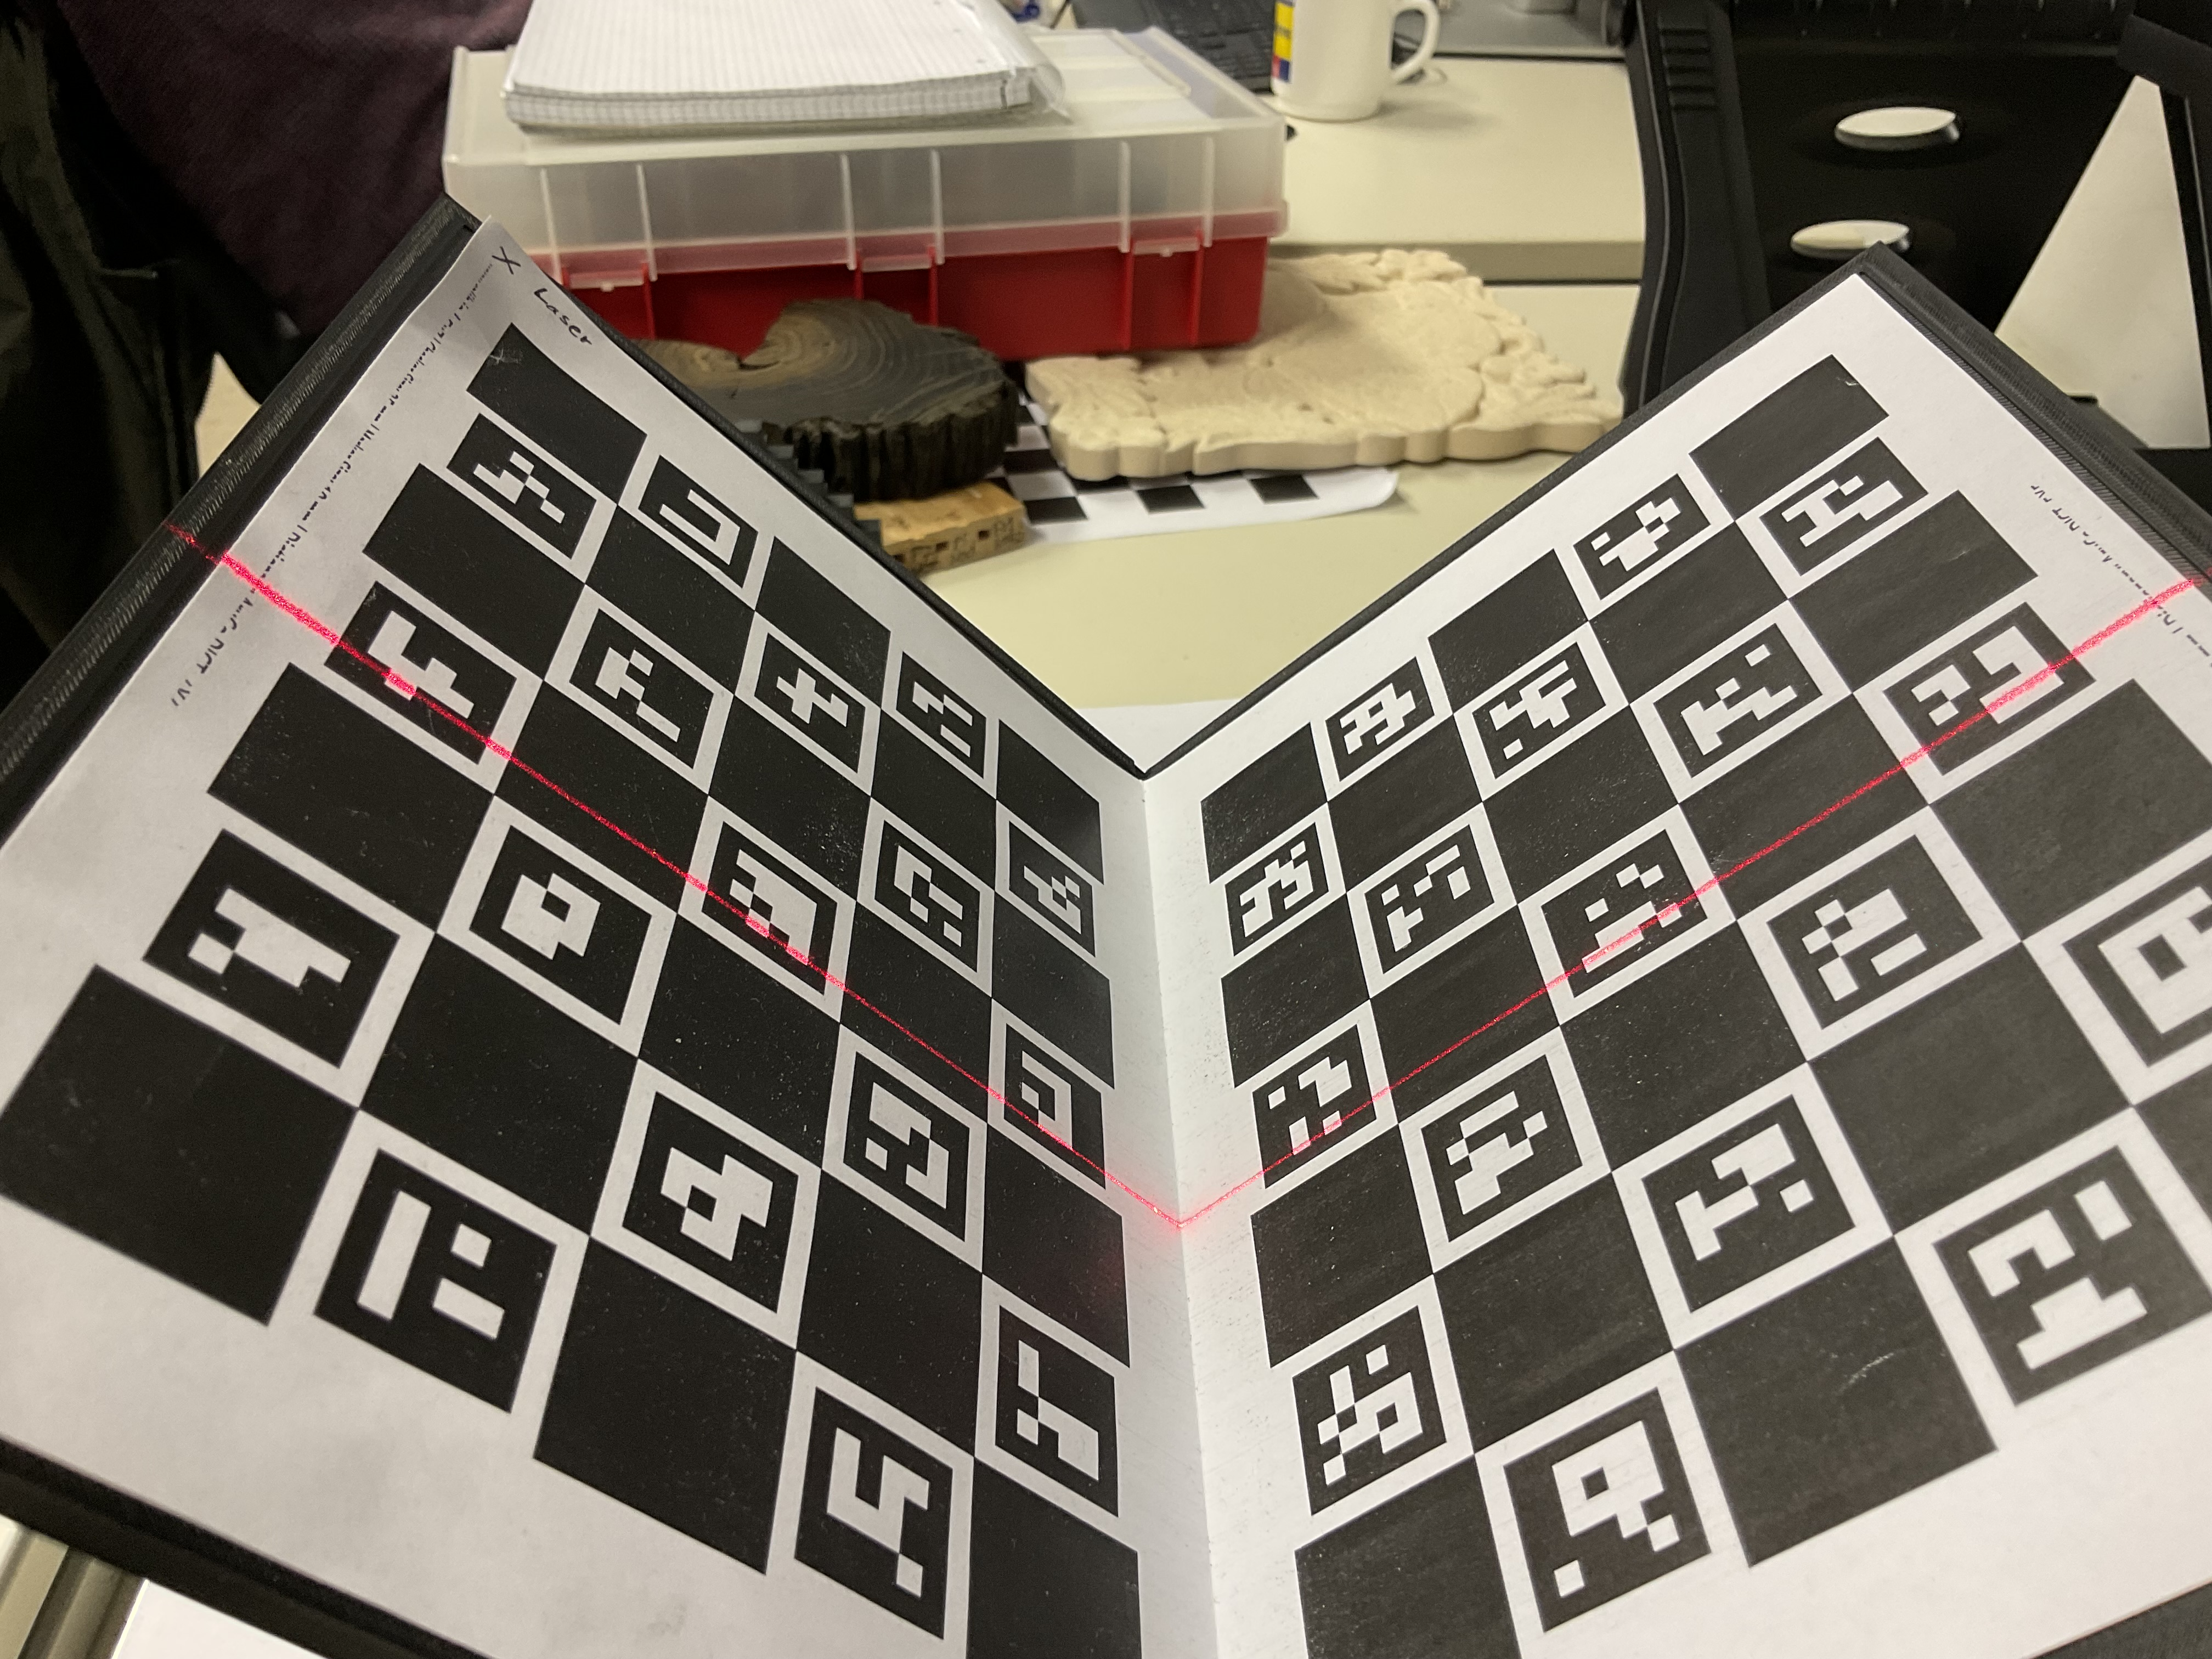
\includegraphics[width=0.49\linewidth]{img/hauptteil/ext-calib/pattern_0.jpg}
			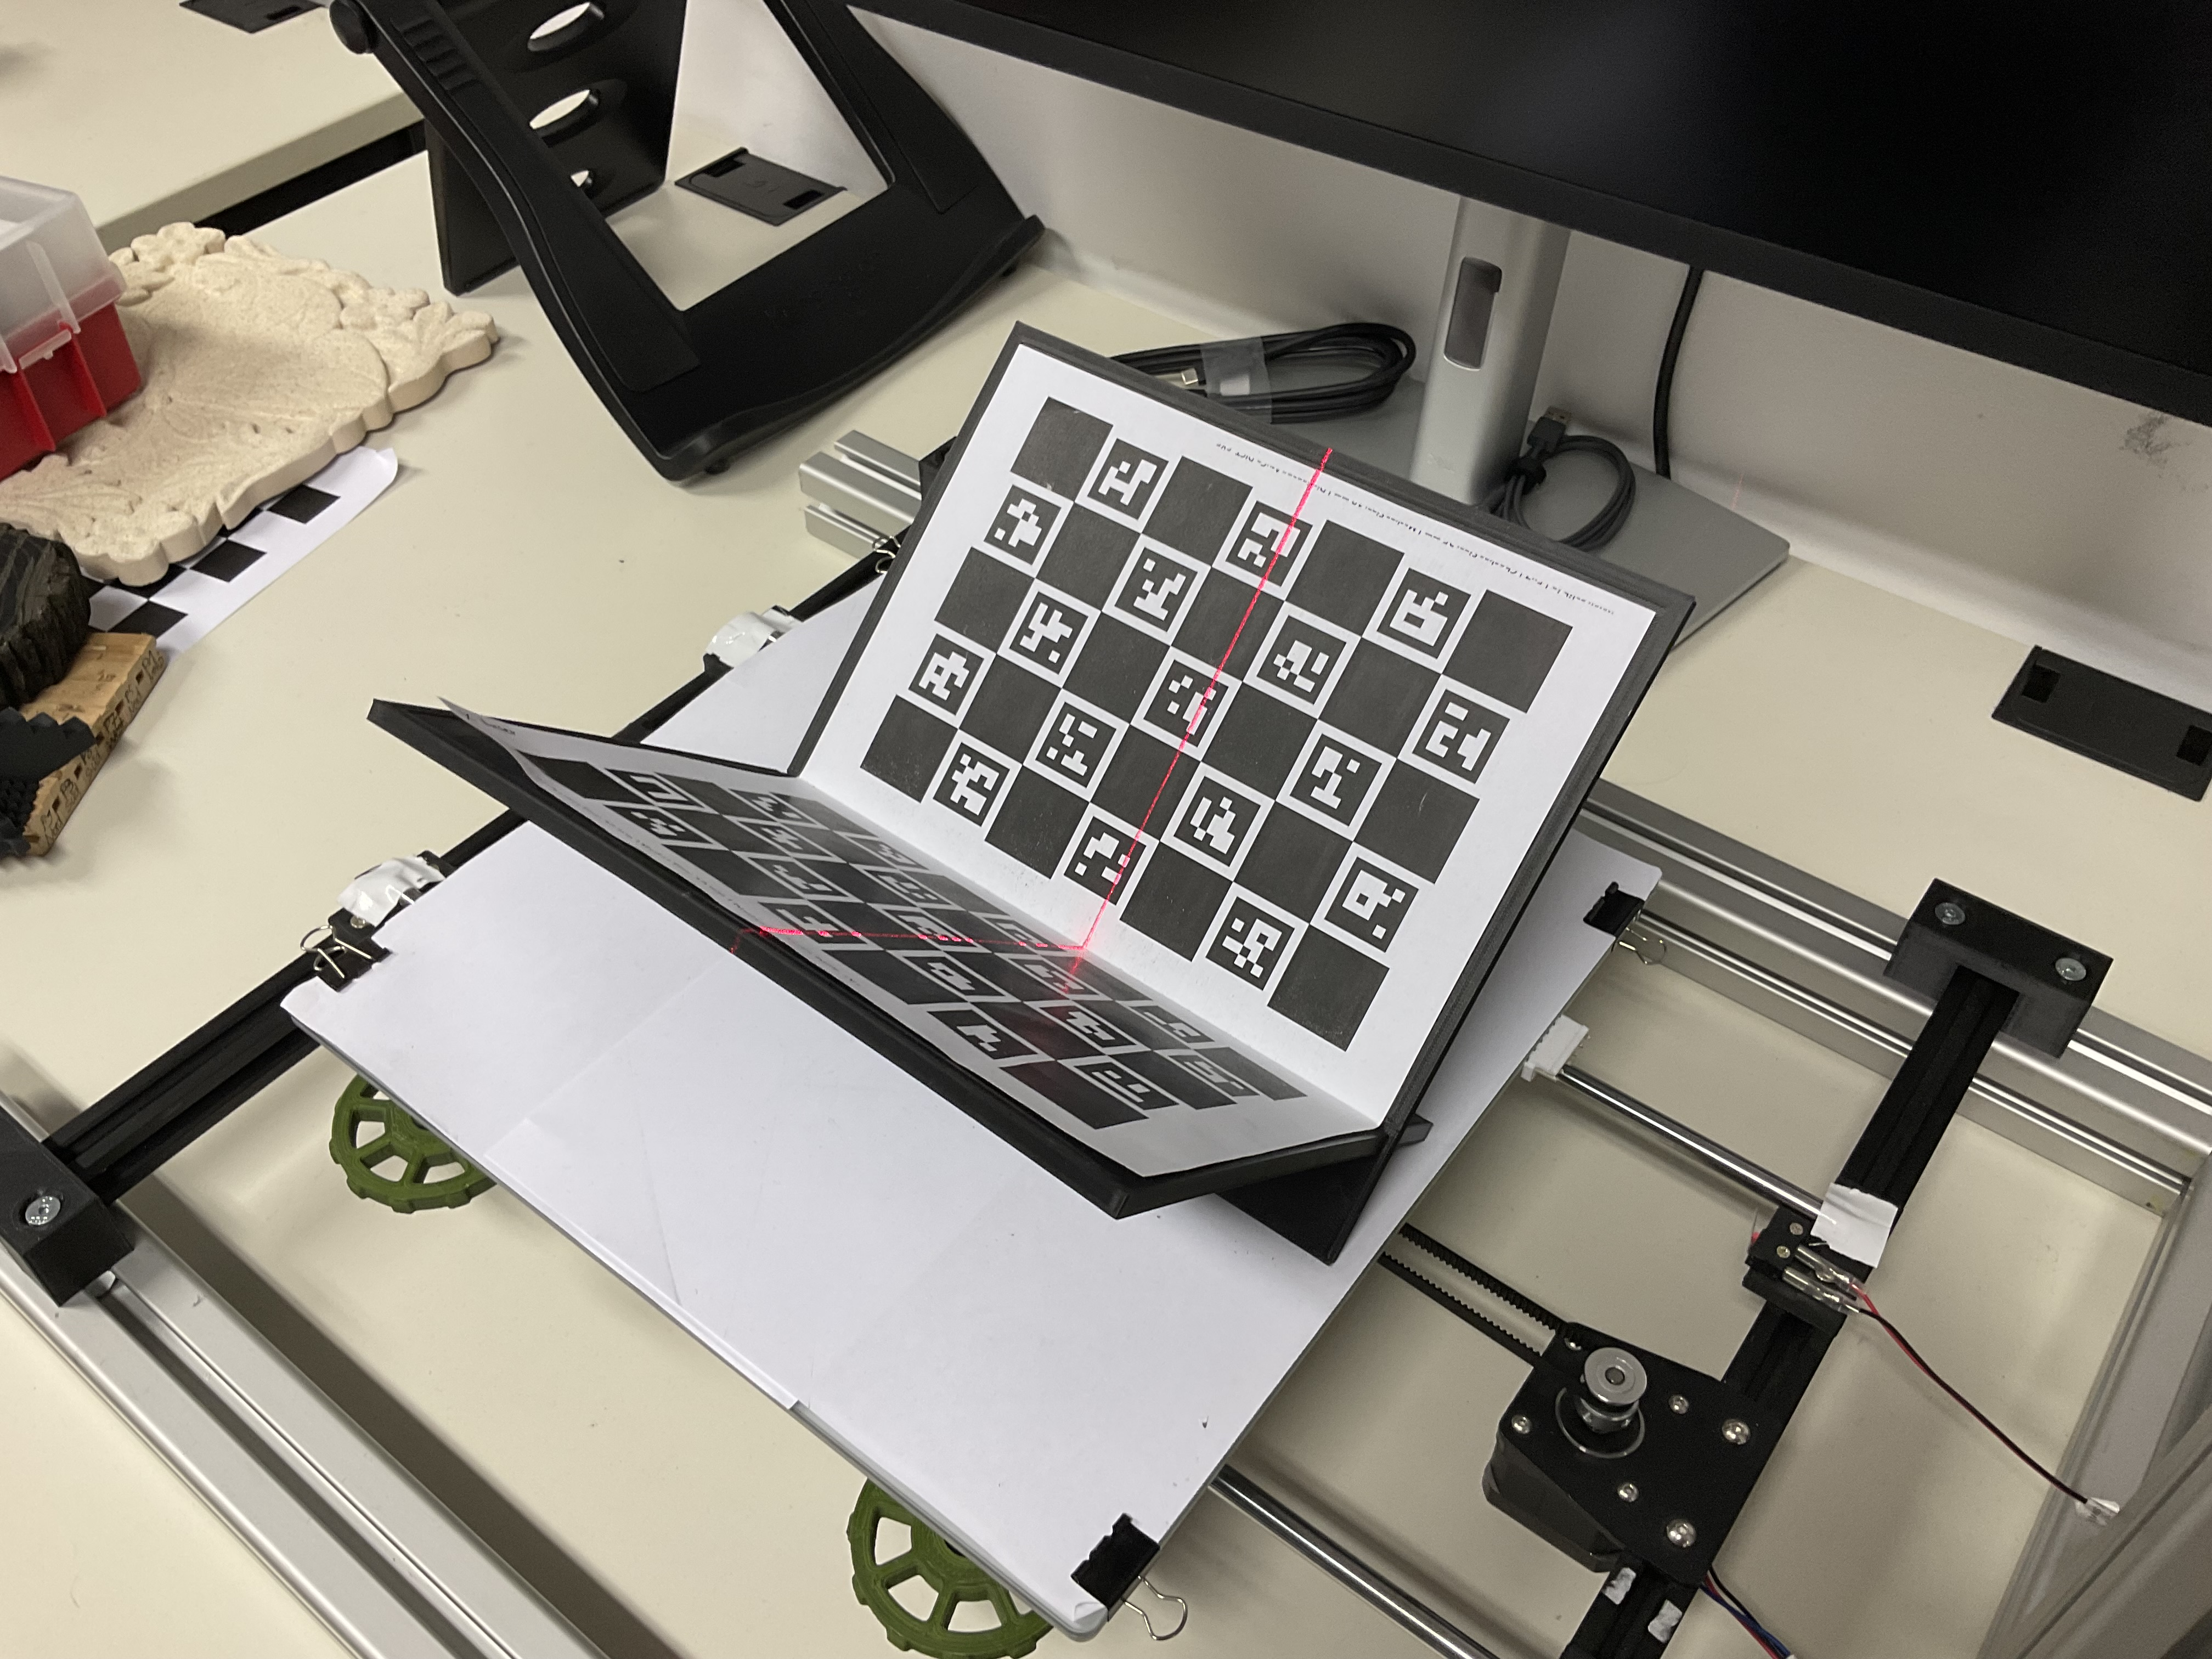
\includegraphics[width=0.49\linewidth]{img/hauptteil/ext-calib/pattern_1.jpg}
			\caption{Unterlage zum Kalibrieren}
			\label{fig:ext-calib-pattern}
		\end{figure} 
	
		In diesem Fall wurde ein 90°-Winkel benutzt. Das Kalibrier-Brett ist über ein 3D-Drucker gedruckt wurden. Diese Bilder sind Beispielbilder. Der entwickelte Lasertriangulationssensor liefert während dem Kalibriervorgang Output-Bilder, die verschiedenen Arbeitsschritte untermalen.
		\begin{figure}[h]
			\centering
			\subfloat[]{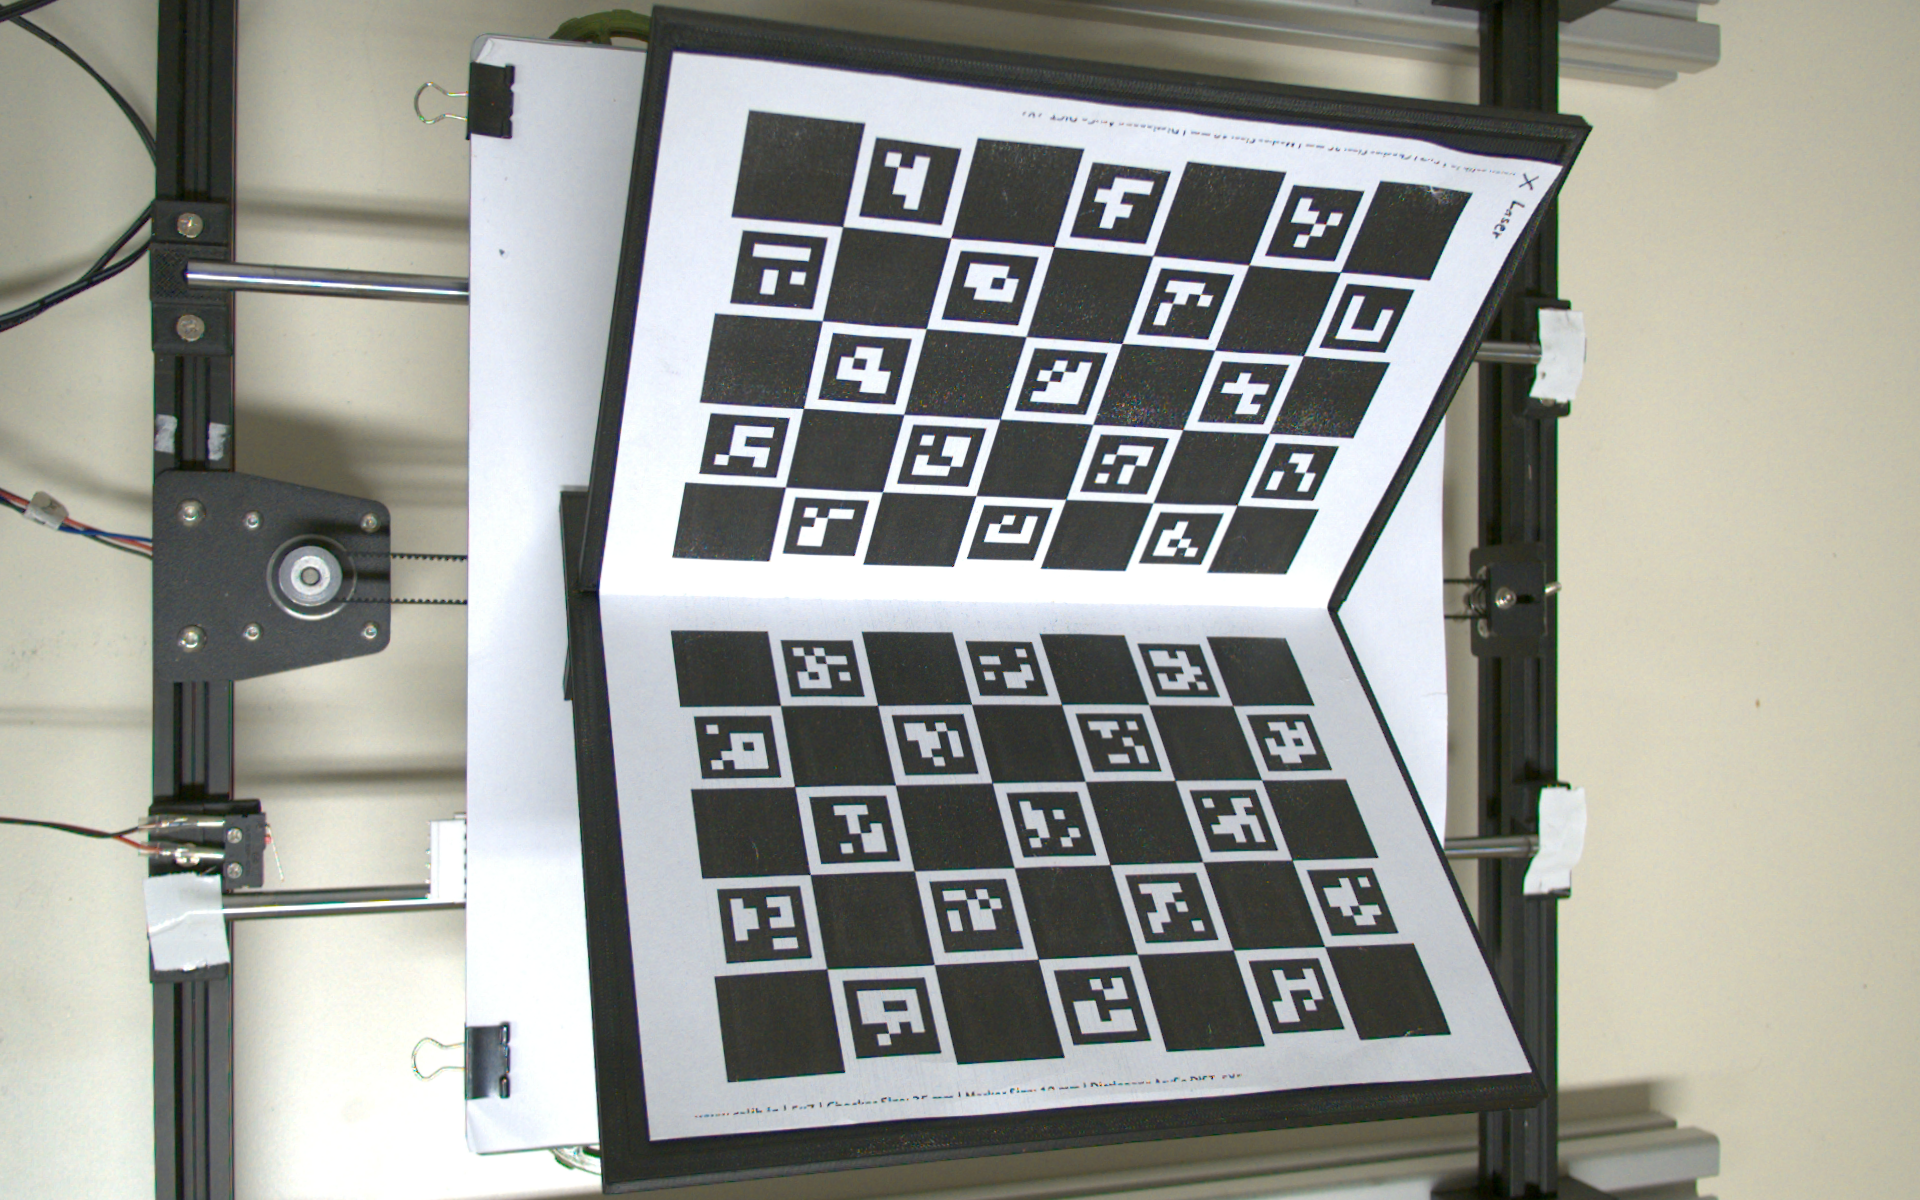
\includegraphics[width=0.49\linewidth]{img/hauptteil/ext-calib/charuco_board.png}
				\label{subfig:raw}}
			\subfloat[]{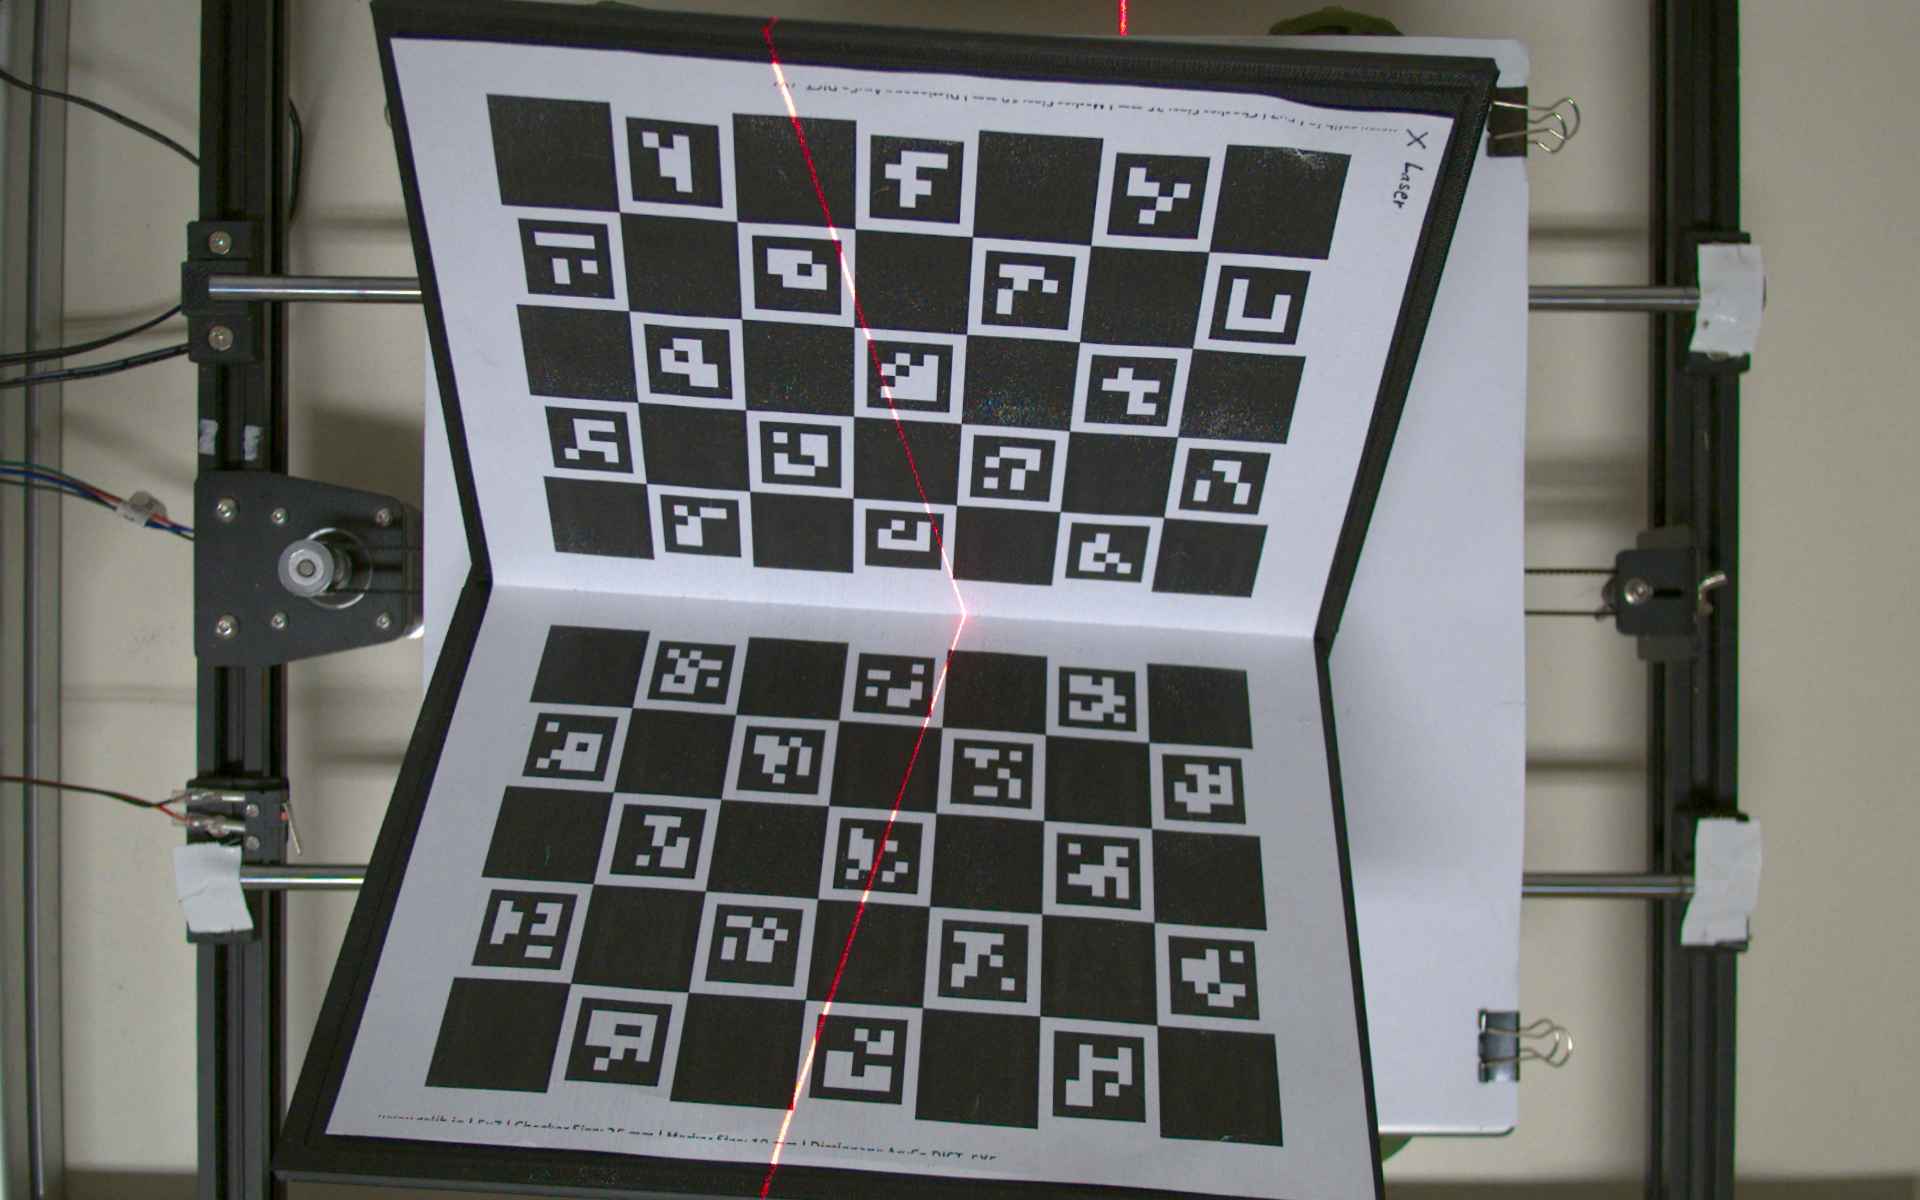
\includegraphics[width=0.49\linewidth]{img/hauptteil/ext-calib/charuco_board_laser.png}
				\label{subfig:raw_laser}}
			\caption{Ausgangsbilder der extrinsischen Kalibrierung}
			\label{fig:ext-calib-raw}
		\end{figure} 
	
		Gemäß Kapitel \ref{chap:bildverarbeitung} wird ein Bild-Paar aufgenommen. In einem ist die Laserlinie sichtbar (Abbildung \ref{subfig:raw_laser})und in dem anderen nicht (Abbildung \ref{subfig:raw}).
		
		$\underline{Unterscheidung \; der \; Schachbretter}$
		
		In den Vorherigen Abbildungen fällt auf, dass es sich bei den verwendeten Kalibriermuster nicht um ein herkömmliches Schachbrett handelt. Das verwendete Muster ist ein ChArUco-Board. Das Problem bei einem herkömmlichen Schachbrett ist, dass der Algorithmus für die Kamera-Kalibrierung in einem einzigen Bild nicht zwischen zwei Schachbrettern unterscheiden kann. Ein ChArUco-Board besitzt in den normal weißen Flächen eines Schachbretts sogenannte ArUco-Marker. Diese Marker können von der Kamera erkannt und eindeutig unterschieden werden. Das finden und unterscheiden der ChArUco-Board ist in OpenCv implementiert. Dabei definiert man, ähnlich zu dem Schachbrett aus der intrinsischen Kalibrierung \ref{chap:kalibrierung_intrinsisch}, im Vorhinein die Parameter des Boards. Dazu gehören nicht nur die Kachel, sondern auch eine gewisse ArUco-Bibliothek, welche die Marker beschreibt. Der Algorithmus kann nun in einem Bild die beiden Boards unterscheiden und platziert ein Koordinatensystem darauf. Vorausgesetzt wird dabei, das die Kameramatrix und die Distortion-Koeffizienten bereits bekannt sind. Da die intrinsische Kalibrierung initial durchgeführt wird, ist diese Voraussetzung erfüllt.  
		
		\begin{figure}[h]
			\centering
			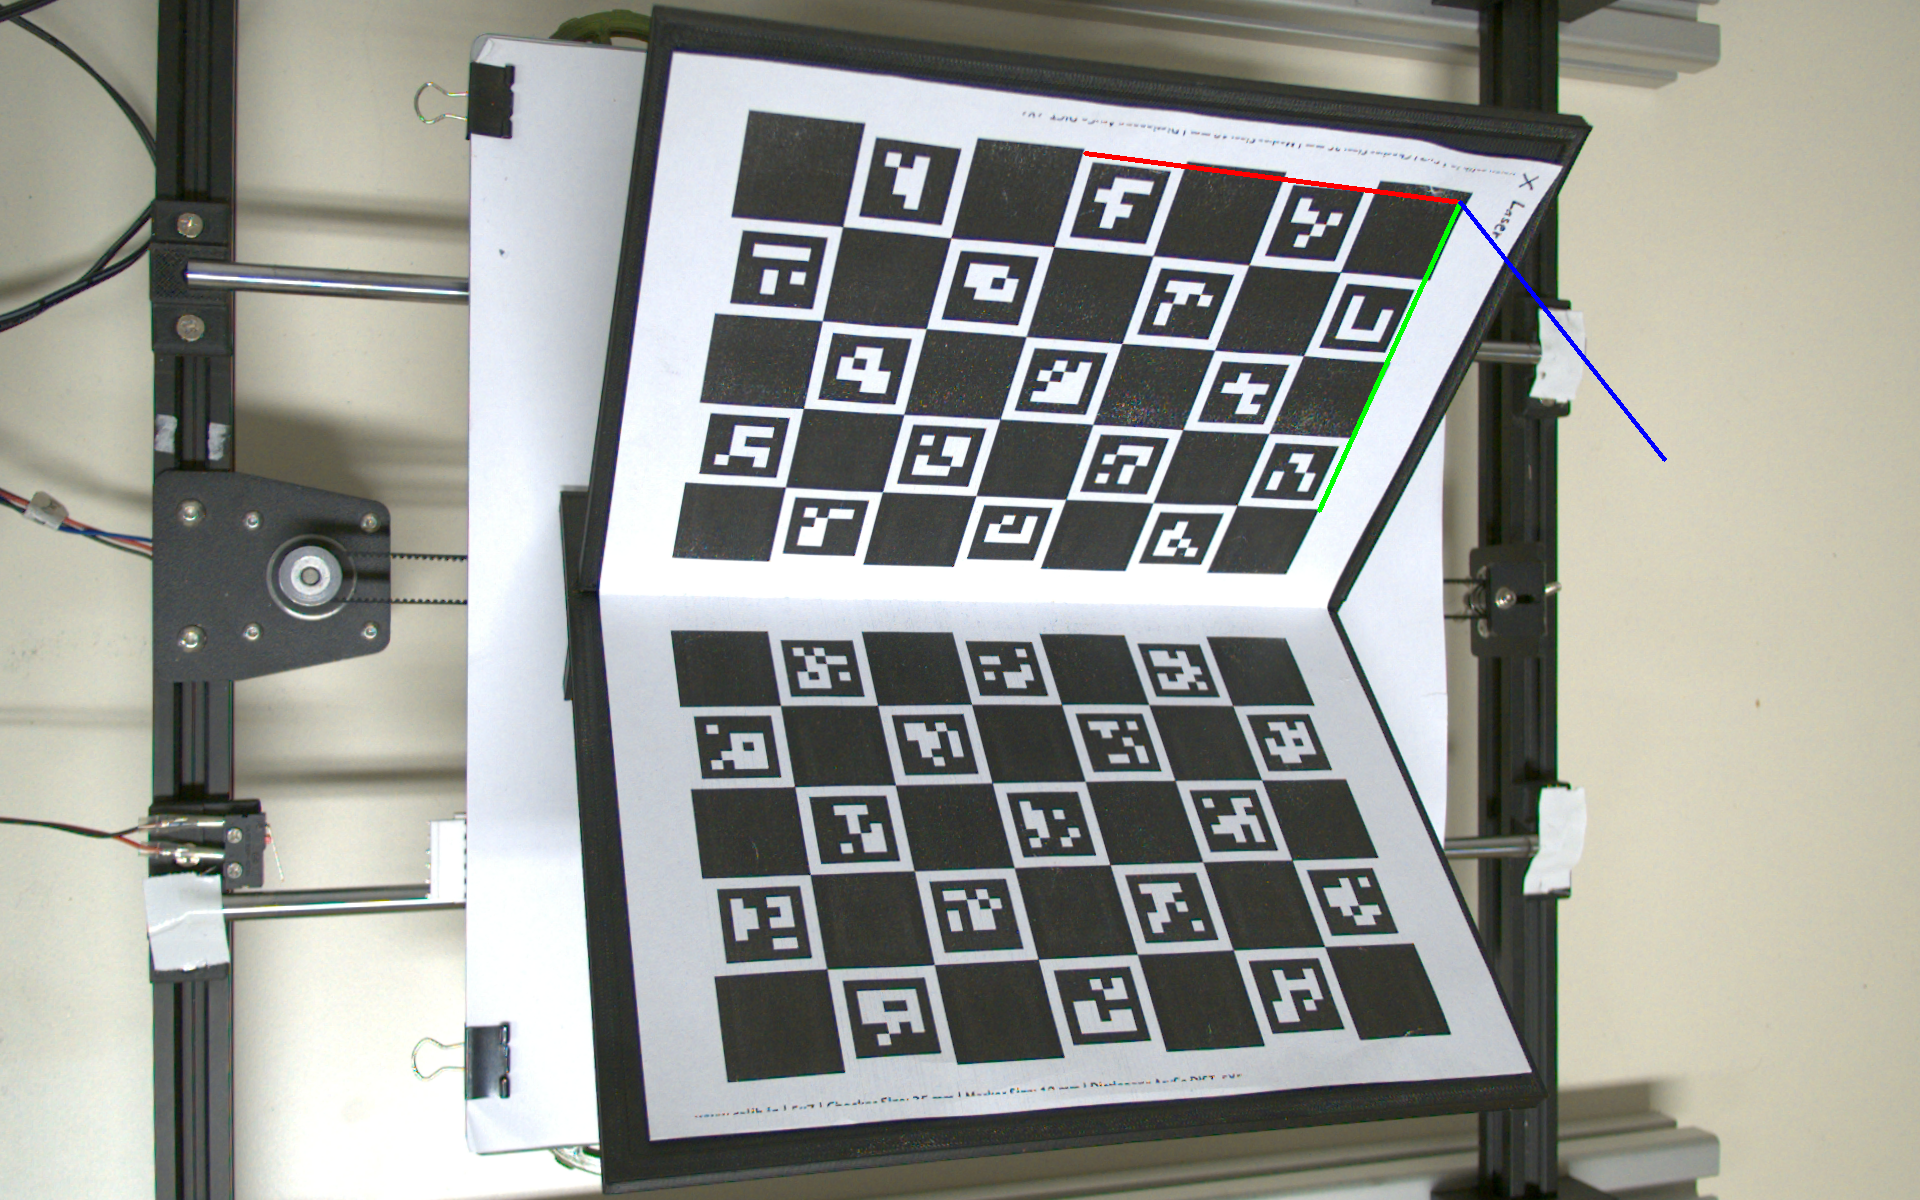
\includegraphics[width=0.49\linewidth]{img/hauptteil/ext-calib/charuco_primary.png}
			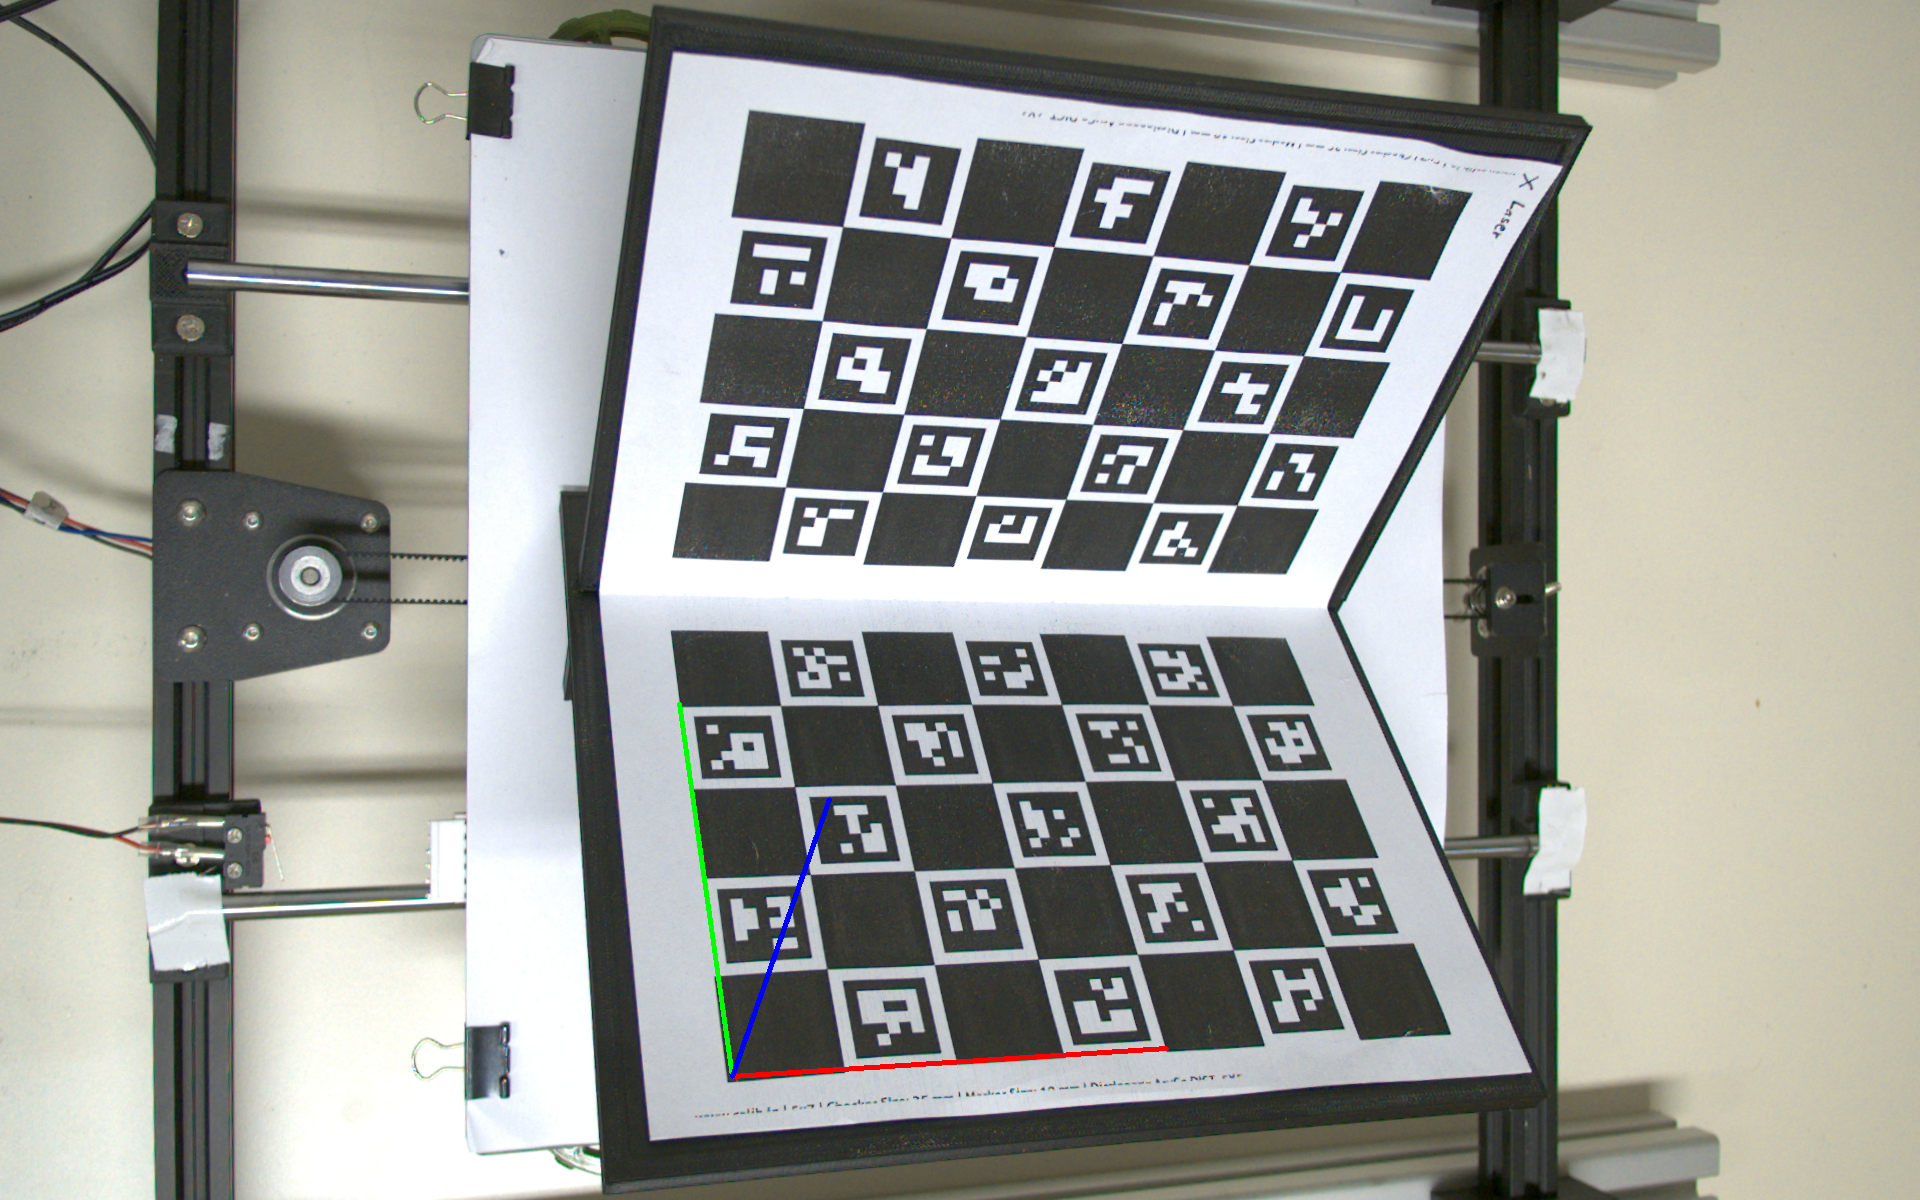
\includegraphics[width=0.49\linewidth]{img/hauptteil/ext-calib/charuco_secondary.png}
			\caption{Weltkoordinatensysteme im ChArUco-Board}
			\label{fig:ext-calib-poses}
		\end{figure}
	
		Bekannt sind jetzt die Rotation und Translation von dem Kamerakoordinatensystem zu den zwei Weltkoordinatensystemen, die aus den ChArUco-Boards folgen.
		
		$\underline{Finden \; der \; richtigen \; Laserlinie}$
		
		Der nächste Schritt muss es sein, die Laserlinie im Bild herauszuarbeiten. Wir wollen die 2D-Punkte der Laserlinie wissen und sie in die 3D-Repräsentation in dem Weltkoordinatensystem umwandeln. Kapitel \ref{chap:bildverarbeitung} beschreibt die Methodik. Das Problem ist, dass nur der Teil der Laserlinie benutzt werden darf, der sich auch tatsächlich auf den jeweiligen Schachbrett befindet. Das bedeutet, dass nur ein gewisser Ausschnitt aus dem Bild wichtig ist. Und zwar genau das zu untersuchende ChArUco-Board. \newline
		Das ChArUco-Board selbst ist dabei die Lösung des Problems. OpenCv erkennt die sowohl die ArUco-Marker als auch die Ecken der Kachel. Dabei besitzen alle eine eindeutige ID. Über die Ecken kann also ein Bereich abgesteckt werden.
		
		\begin{figure}[h]
			\centering
			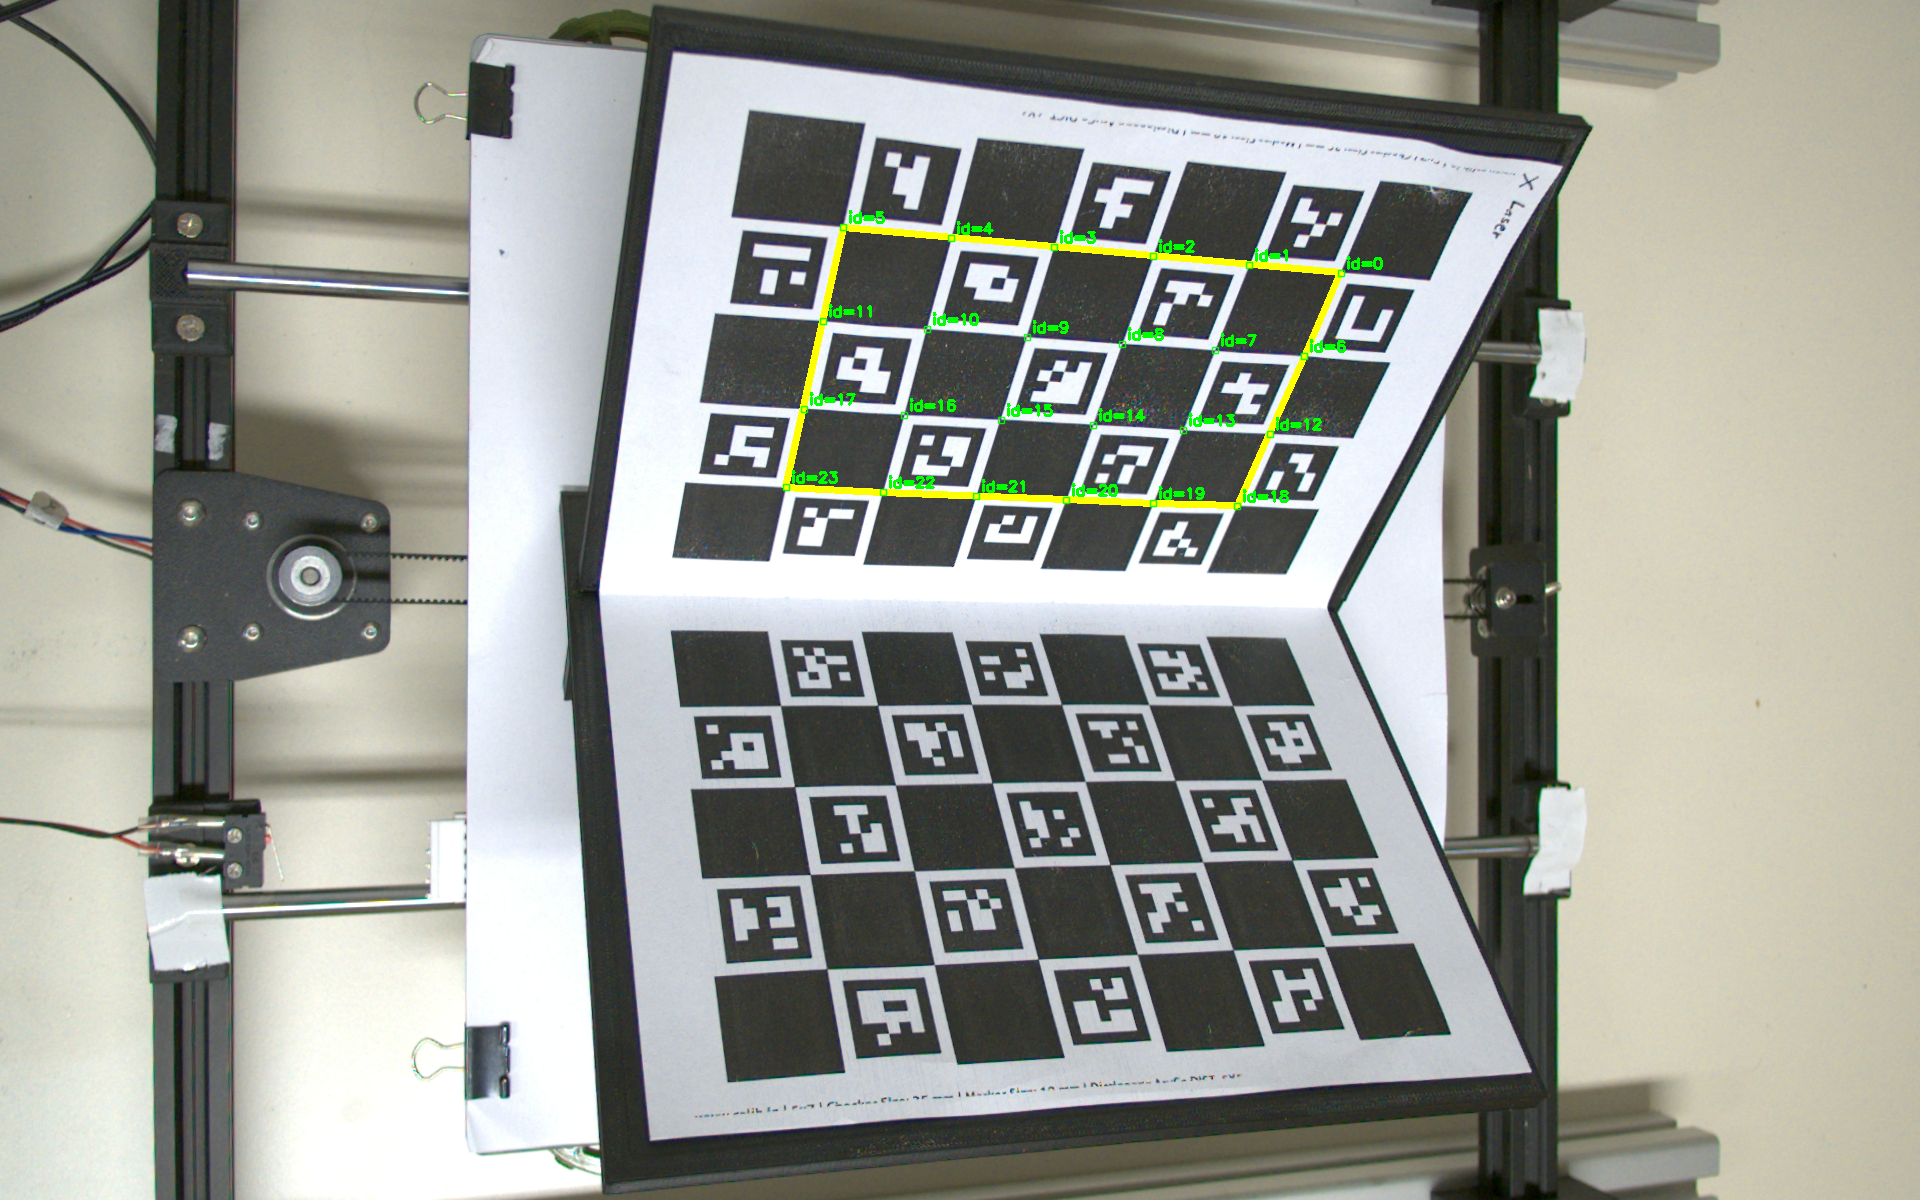
\includegraphics[width=0.8\linewidth]{img/hauptteil/ext-calib/charuco_convex_hull_primary.png}
			\caption{Point of Interest im Bild}
			\label{fig:ext-calib-hull}
		\end{figure}
	
		Um den wichtigen Bereich abzustecken sind die Eckpunkte des Bereiches mit den IDs 0, 5, 18 und 23 ausschlaggebend. Wegen Fehleranfälligkeit wurde jedoch davon abgesehen, genau diese Ecken anzusprechen. Falls in einem Bild eine der äußeren Ecken nicht erkannt wurde, könnten man so den Bereich nicht abstecken. Deswegen wird eine Konvexe Hülle benutzt. Damit werden immer die äußersten Punkte berücksichtigt. Fall gewisse Ecken wegen einer Unschärfe im Bild nicht erkannt werden, führt das nun nicht zu Fehlern. In Abb. (\ref{fig:ext-calib-hull}) ist die abgesteckte Fläche in Gelb eingezeichnet. Falls keine Ecke bzw. keine ID gefunden wurden, ist kein ChArUco-Board erkennbar und die Kalibrierung bricht ab. \newline
		Mit den Bekannten Bereich kann eine Maske entwickelt werden, die auf das Bild angewandt werden kann. Die Maske besteht dabei aus einem schwarzen Bild, in dem der ausschlaggebende Bereich aus weißen Pixeln besteht. Wenn man das Ziel-Bild bitweise mit der Maske verundet, bleibt nur der markierte Bereich im bestehen. Alle andern Pixel sind schwarz. Ausgehend von den Ursprungsbildern (Abb. \ref{fig:ext-calib-raw}) werden für die verschiedenen ChArUco-Boards eine Maske entwickelt und angewandt. Das Ergebnis ist die folgende Abbildung.
		
		\begin{figure}[h]
			\centering
			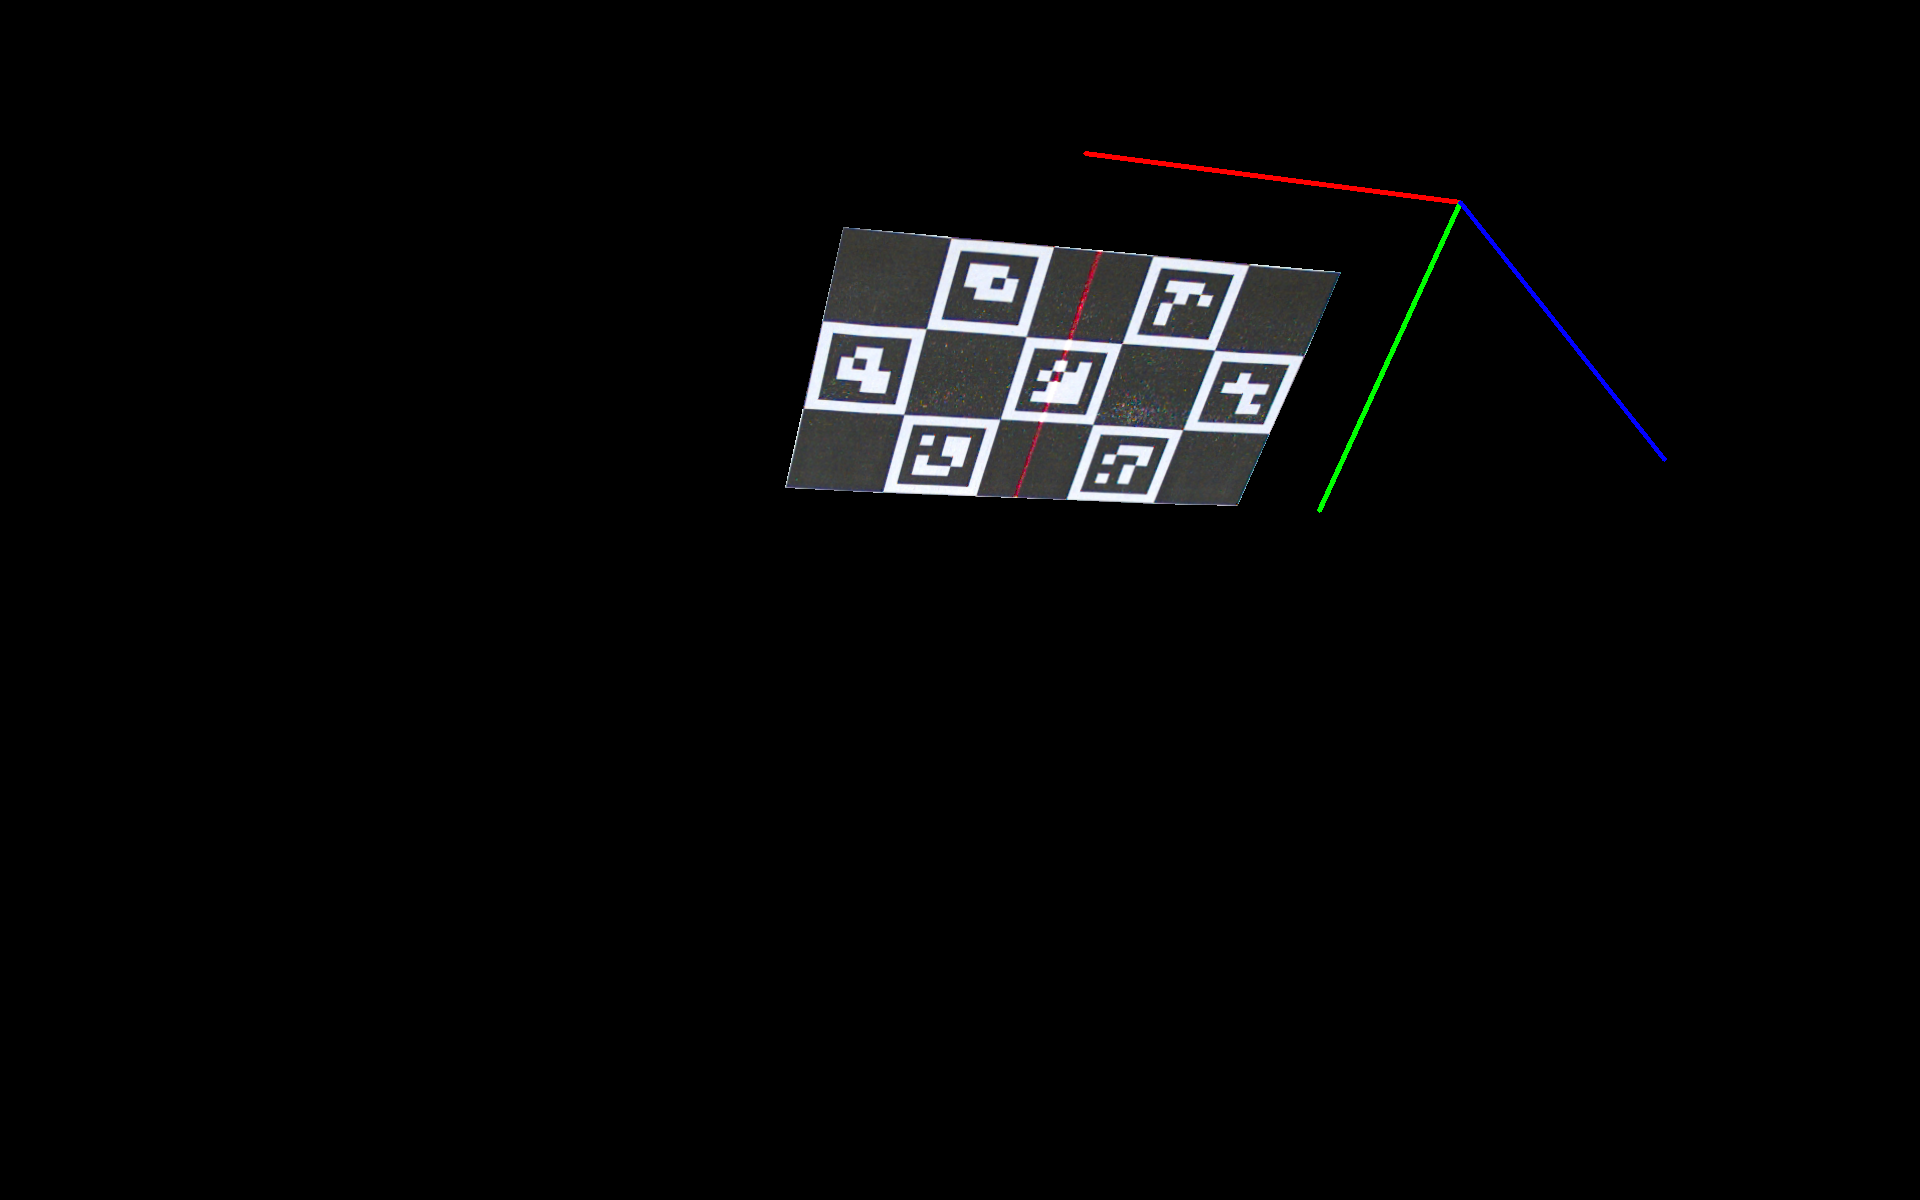
\includegraphics[width=0.49\linewidth]{img/hauptteil/ext-calib/charuco_cut_primary.png}
			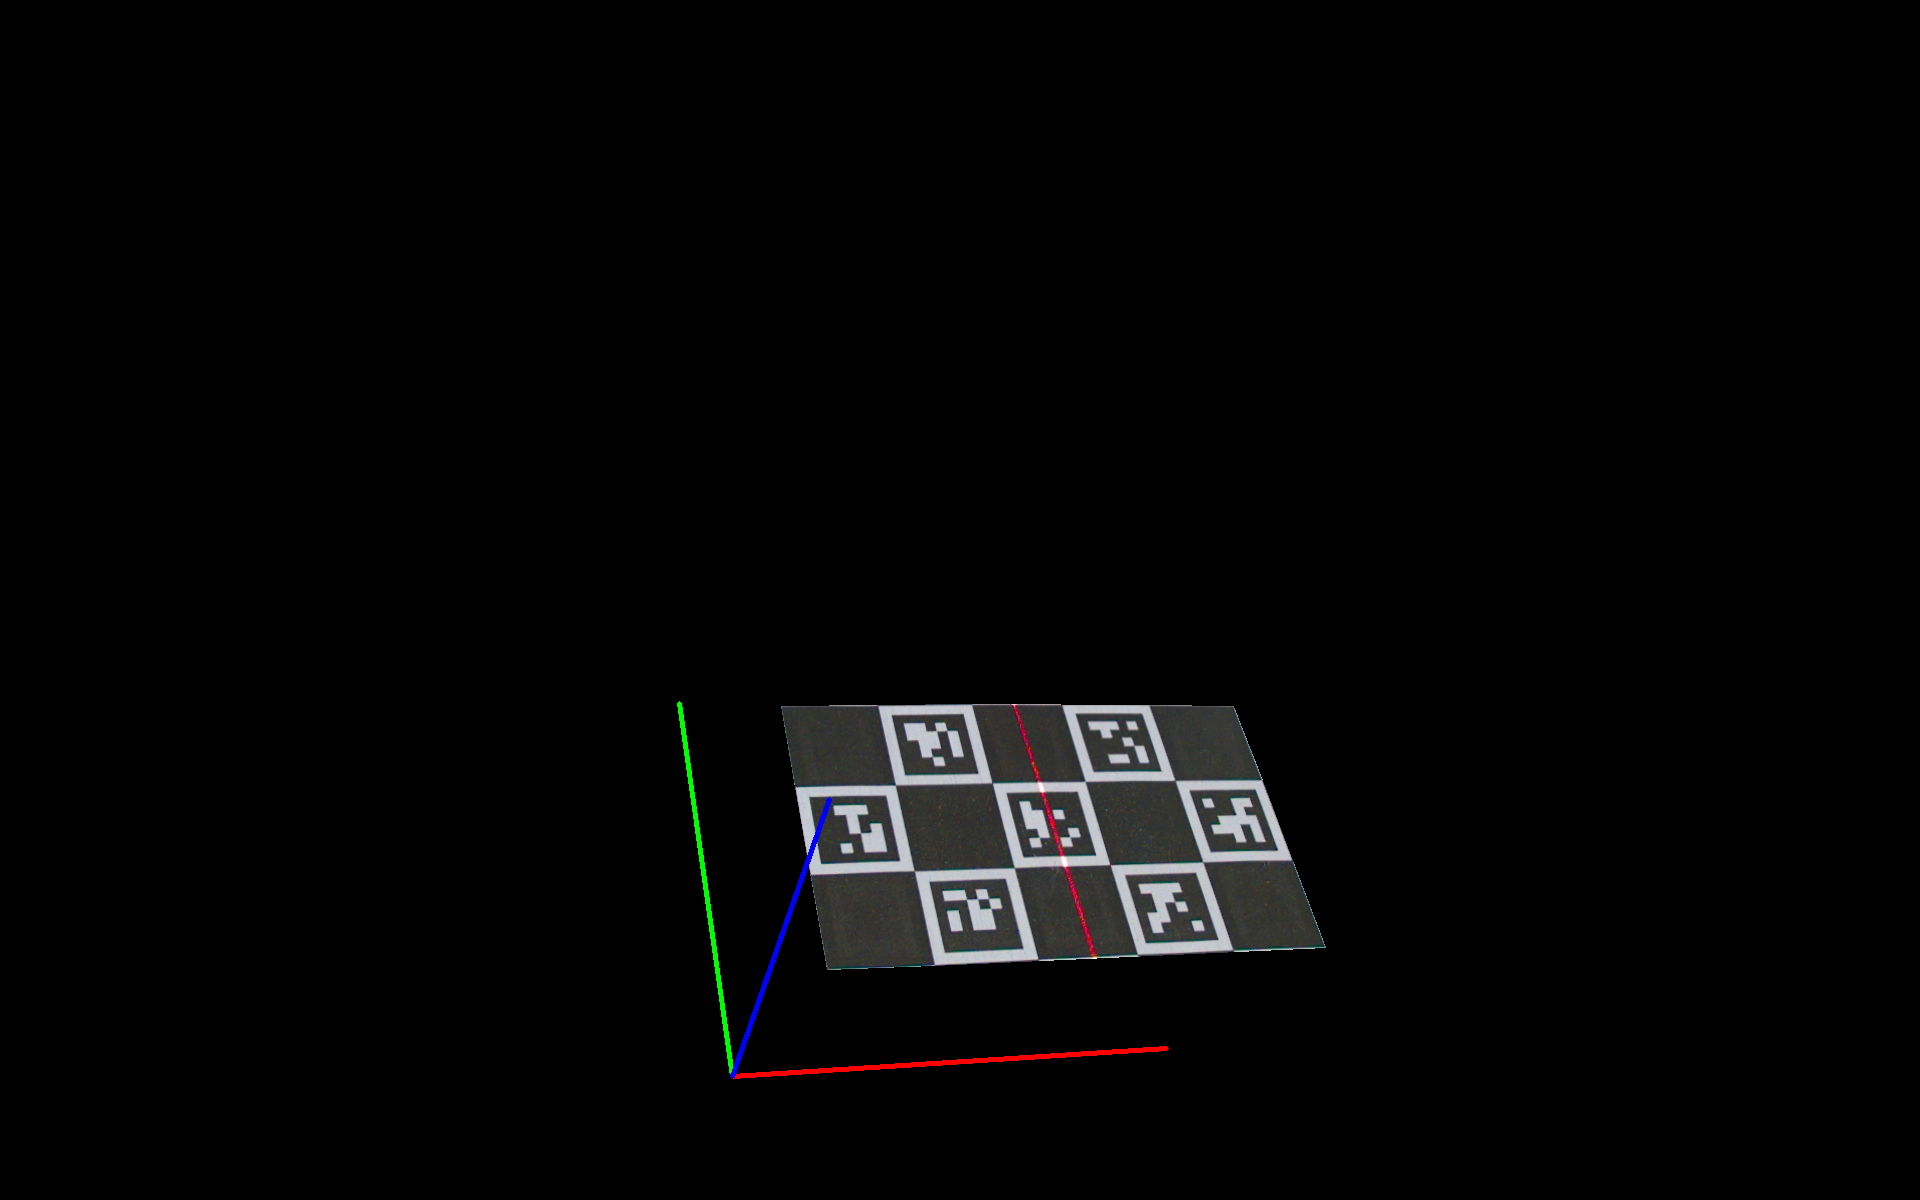
\includegraphics[width=0.49\linewidth]{img/hauptteil/ext-calib/charuco_cut_secondary.png}
			\caption{Ausgeschnitten Laserlinien}
			\label{fig:ext-calib-cut}
		\end{figure}
	
		Die Achsen des jeweiligen Koordinatensystems sind dabei nur zu Übersicht eingezeichnet und nicht Teil der Bildverarbeitung. Verdeutlicht werden soll jedoch, dass das Weltkoordinatensystem bekannt ist. \newline
		Die erstellte Maske kann auch auf das Ursprungsbild ohne Laser angewandt werden. Die beiden ausgeschnittenen Bilder werden an den Algorithmus zum Finden der Laserlinie (Kapitel \ref{chap:bildverarbeitung}) weitergegeben. Die nächste Abbildung zeigt das Ergebnis des Subtrahierens der Bilder. Zur Übersicht sind wieder die Koordinatenachsen eingetragen. Tatsächlich sind an diesem Punkt als Ergebnis der Bildverarbeitung schon die Subpixel der Laserlinie bekannt. Subpixel sind schwierig in einem Bild darzustellen, deshalb wurde sich für das Zeigen des Zwischenschritts entschieden.
	
		\begin{figure}[h]
			\centering
			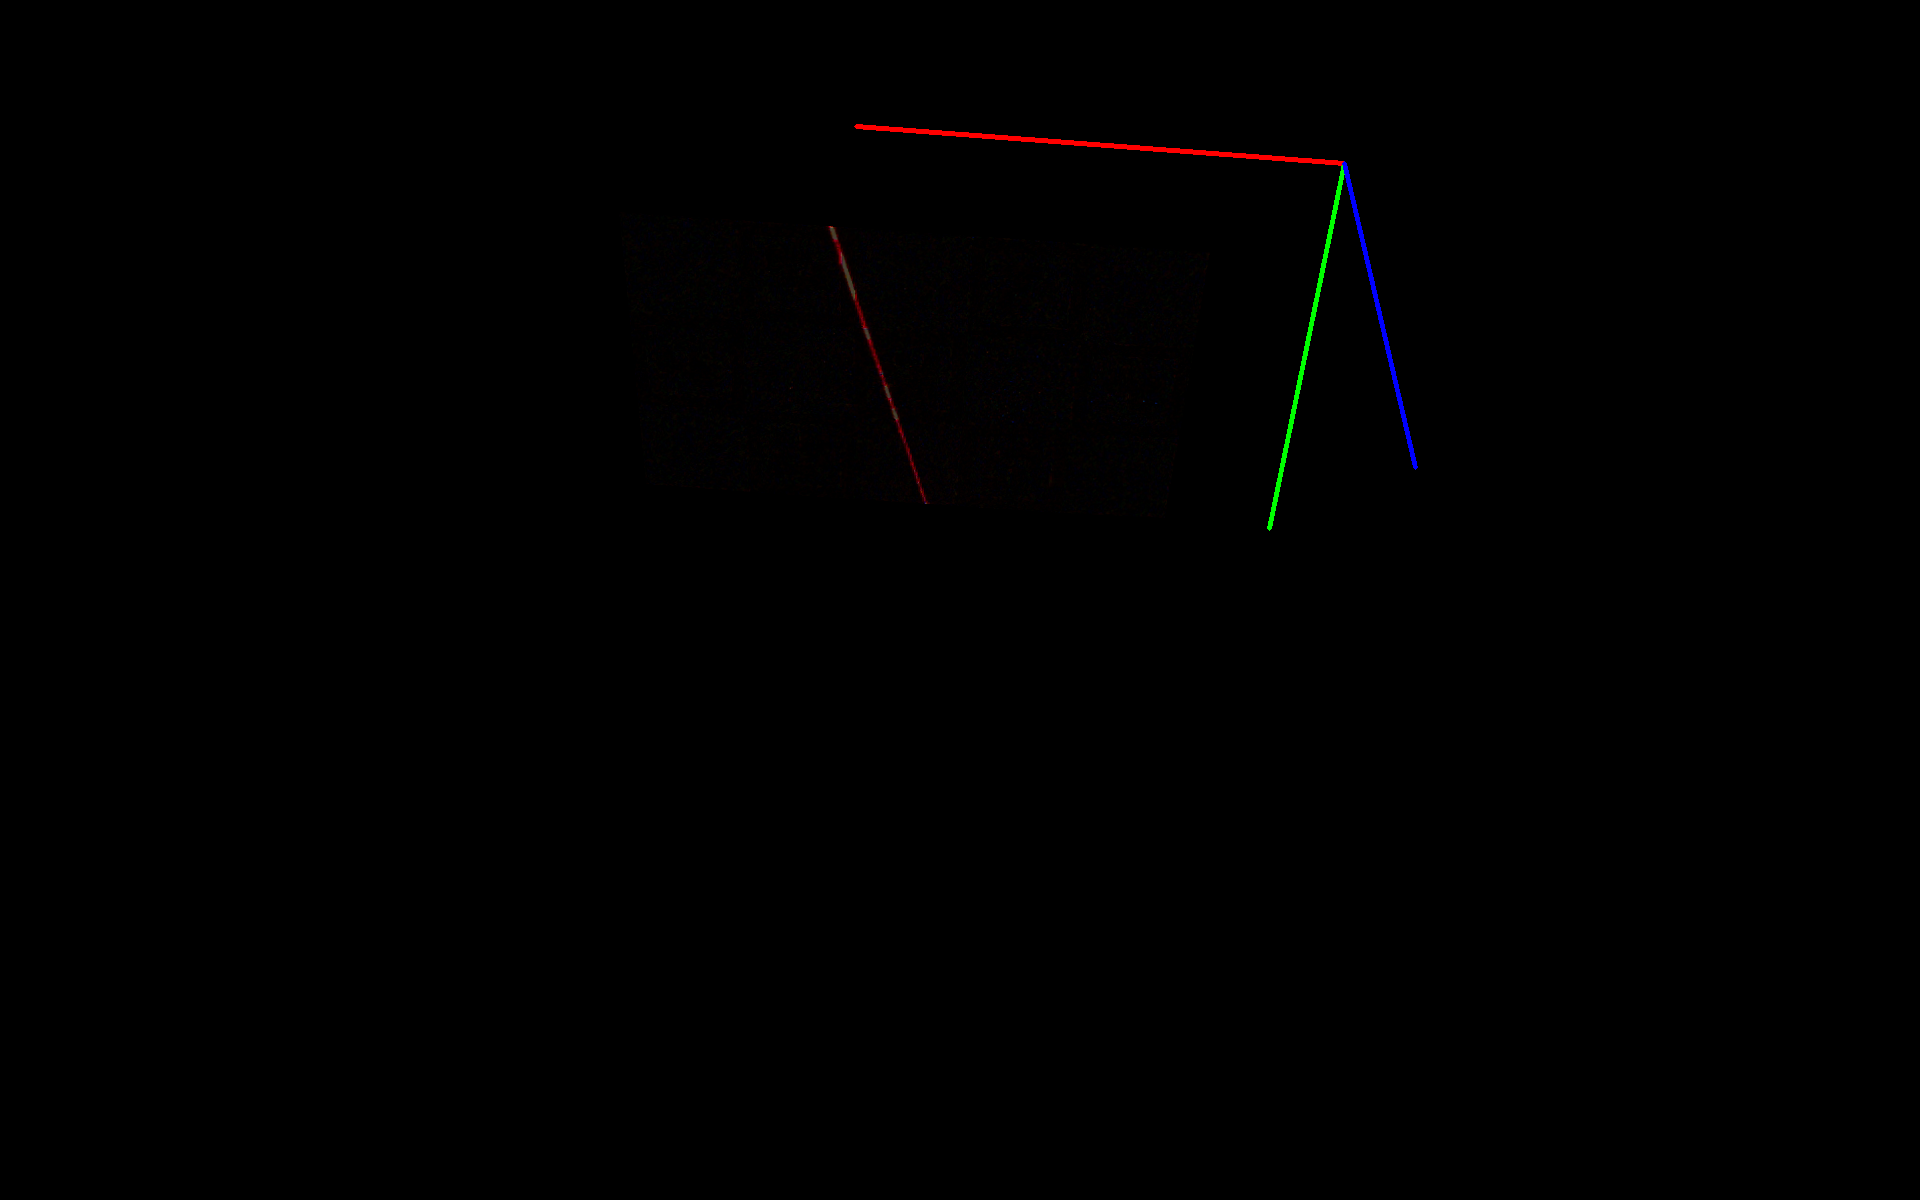
\includegraphics[width=0.49\linewidth]{img/hauptteil/ext-calib/laserline_primary.png}
			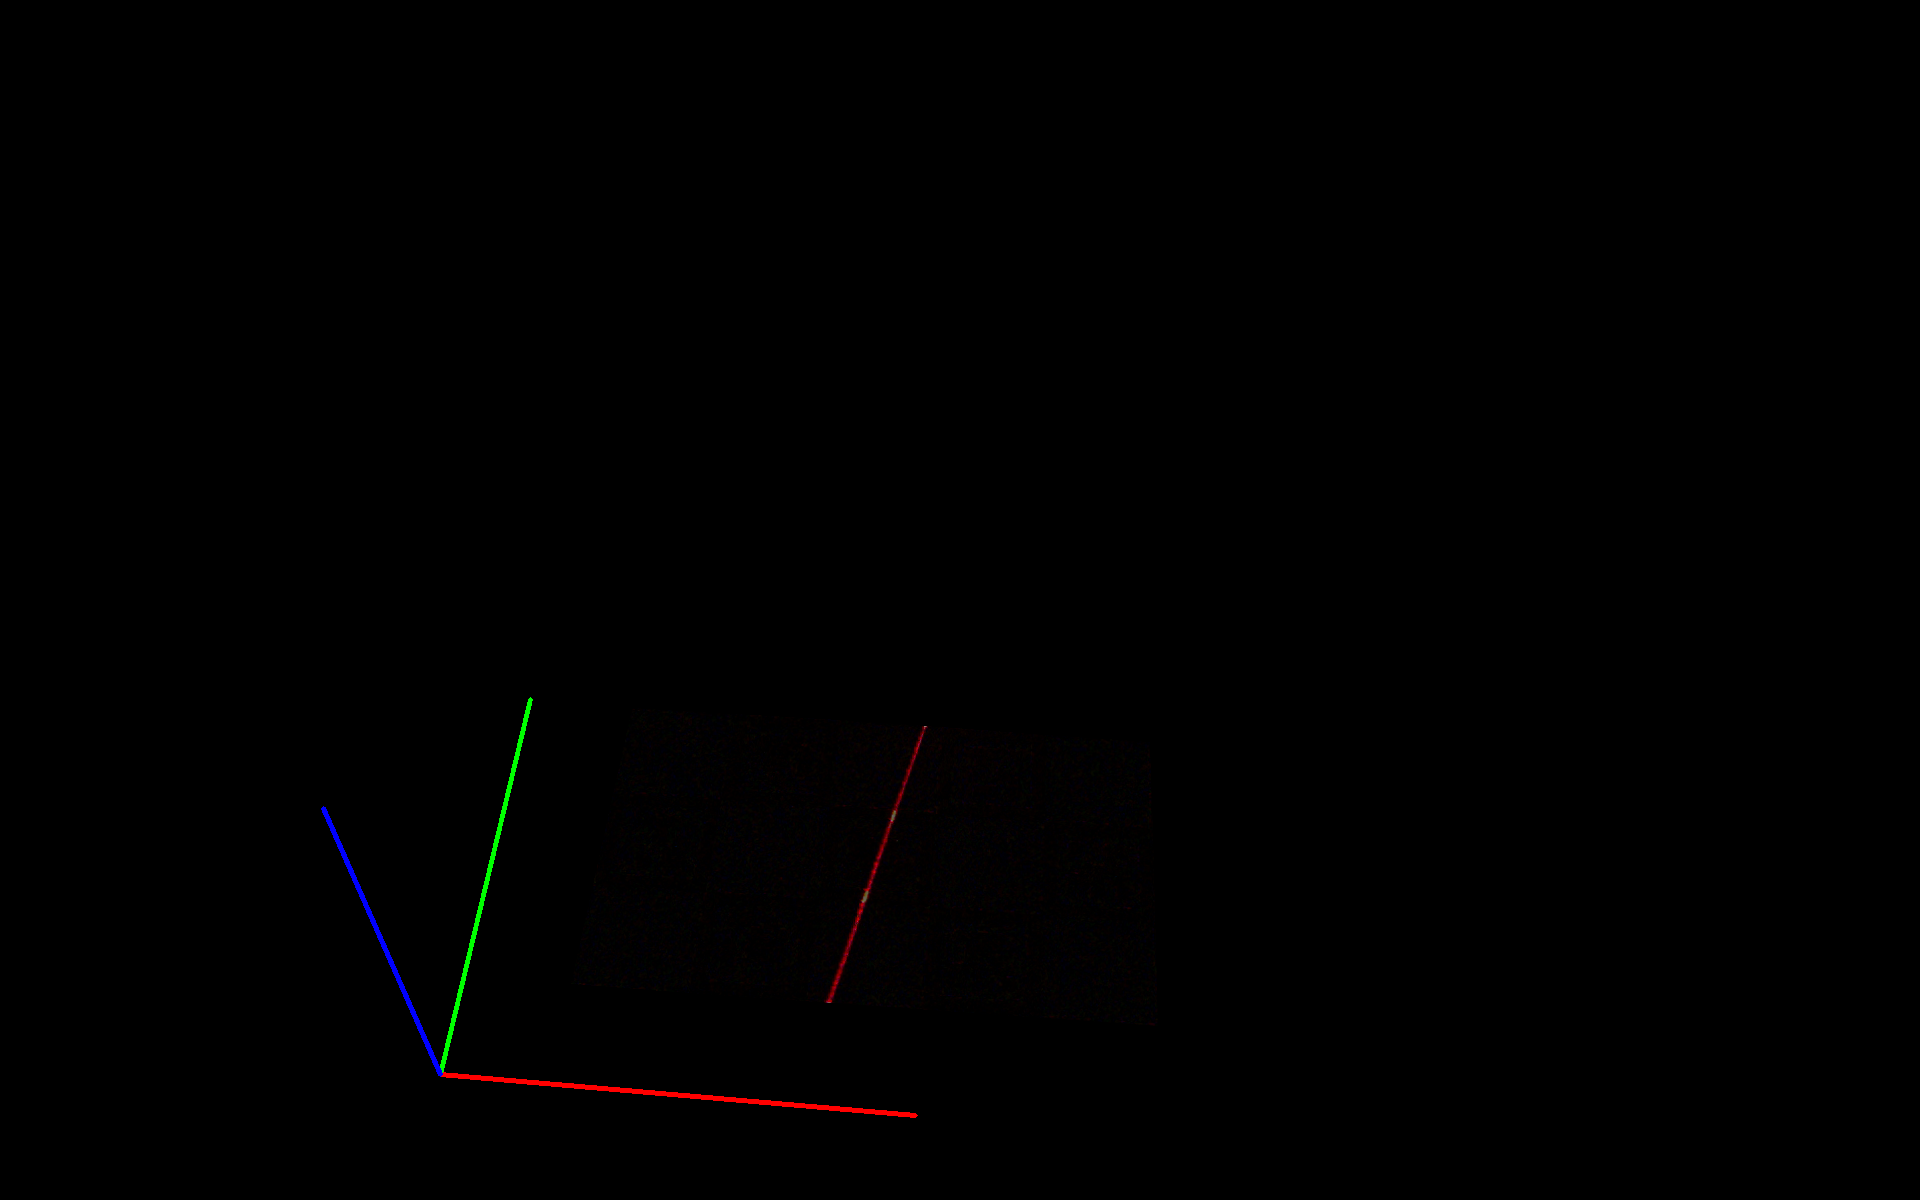
\includegraphics[width=0.49\linewidth]{img/hauptteil/ext-calib/laserline_secondary.png}
			\caption{Herausgearbeitete Laserlinien}
			\label{fig:ext-calib-laserlines}
		\end{figure}
	
		$\underline{Der \; Scale-Factor}$
		
		An diesem Punkt kommt es zum Einsatz der Formel für die 3D-Weltkoordinaten (\ref{eq:basic_trans}). Wie in den Kapitel \ref{chap:transformationen} angemerkt, ist der Scale-Factor noch eine Unbekannte, die gefunden werden muss. Ohne sie wäre die Gleichung noch nicht lösbar. Dieses Problem kann wie folgt umgangen werden. Das Weltkoordinatensystem wird auf das ChArUco-Board gelegt. Die Laserlinie liegt ebenfalls genau auf dem Board. Das bedeutet, dass die Z-Koordinate der Laserlinien-Punkte 0 ist. Zu sehen ist das auch in Abb. \ref{fig:ext-calib-laserlines}. Die Laserlinie liegt in der XY-Ebene. Die Z-Koordinaten der Weltkoordinatenpunkte müssen 0 sein. Mit dem Ausgangspunkt von Gleichung (\ref{eq:pixel_zu_welt}) folgt daraus diese Umstellung:
		
		\begin{equation}
			\begin{aligned}
				p_w &= s \; \vec{a} - \vec{b} \\
				das \; entspricht: \\
				x &= s \; a_x - b_x \\
				y &= s \; a_y - b_y \\
				z &= s \; a_z - b_z \\
				mit \; z &= 0: \\
				0 &= s \; a_z - b_z \\
				s &= \frac{b_z}{a_z}
			\end{aligned}
		\end{equation}
		
		Damit ist die Basistransformationsgleichung lösbar und die 3D-Punkte können errechnet werden. Damit nun eine Ebene in die Punkte gelegt werden kann, müssen alle Punkte in ein einheitliches Koordinatensystem gelegt werden. Durch die bekannten Transformationen ist dies jedoch kein Problem. Zuerst werden mit (\ref{eq:welt_zu_kamera}) und der eigene Rotation und Translation die Weltpunkte der unteren Laserlinie in das Kamerakoordinatensystem transformiert. Danach wird (\ref{eq:kamera_zu_welt}) genutzt, um mit der Rotation und Translation der oberen Laserlinie die Punkte in das obere Koordinatensystem zu bringen. Die folgende Abbildung gilt als Symbolbild.
	
		\begin{figure}[h]
			\centering
			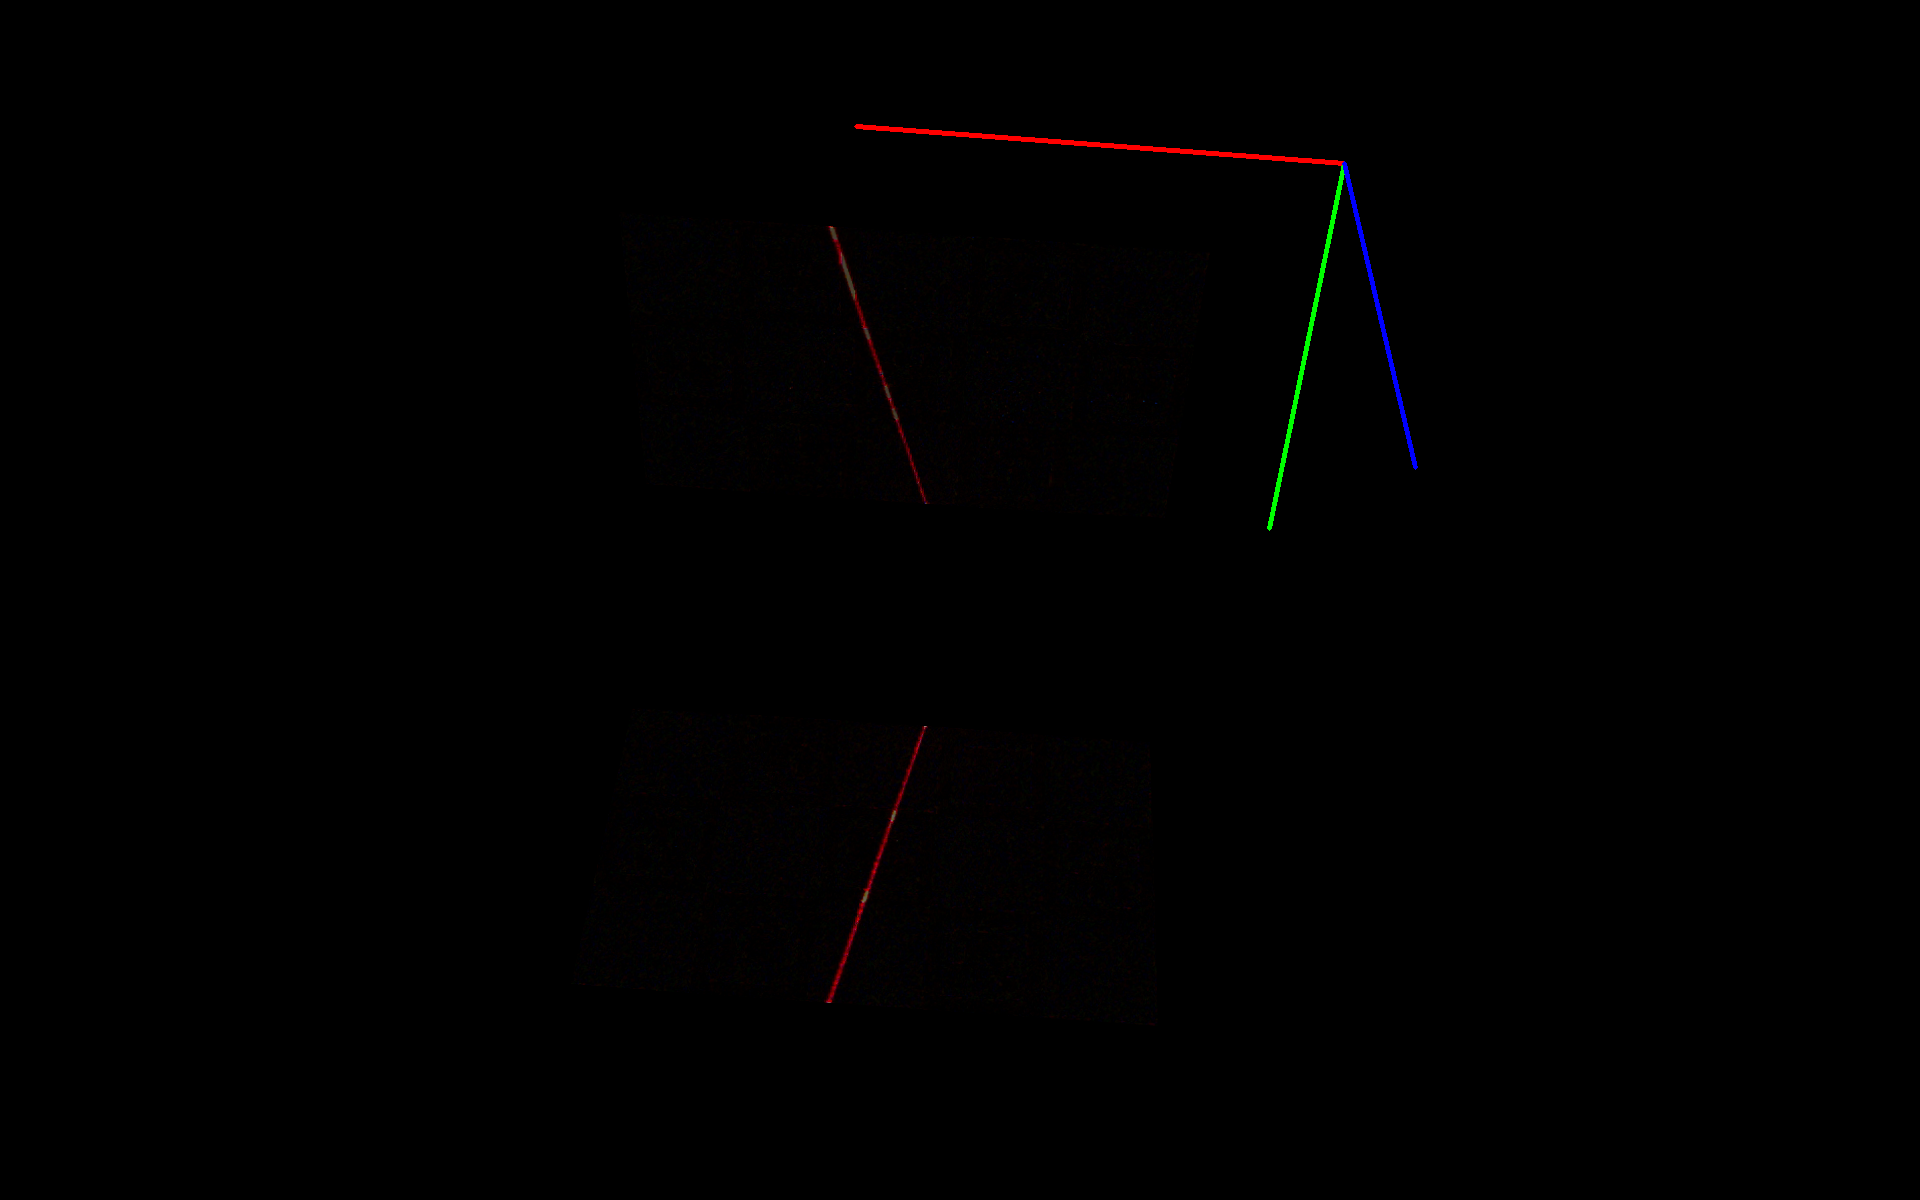
\includegraphics[width=0.85\linewidth]{img/hauptteil/ext-calib/laserline_together.png}
			\caption{Laserlinien in einem Koordinatensystem}
			\label{fig:ext-calib-laserlines-together}
		\end{figure}
	
		$\underline{Das \; Bestimmen \; der \; Ebenengleichung}$
		
		Mit dem letzten Schritt wird die gesuchte Ebenengleichung gefunden. Alle Vorbereitungen sind abgeschlossen. Die richtigen Punkte der zwei nicht parallelen Laserlinien sind in einem einheitlichen Koordinatensystem. Im letzten Schritt muss in diese Punkte eine Ebene gefittet werden. Für einen Ebenen-Fit gibt es diverse Möglichkeiten. Hier wurde sich für die Singular Value Decomposition (SVD) entschieden [svd-t]. Sie ist über die Numpy-Bibliothek in Python implementiert und nutzbar. Wenn man über Numpy den SVD-Algorithmus anwendet, gibt dieser, wie in [svd-t] beschrieben drei Matrizen zurück. Diese heißen U, S und V. Nach [svd-fit] ist die dritte Zeile von U der Normalen-Vektor (\( \vec{n} \)) der passenden Ebene. Ziel ist es eine Ebenengleichung als Koordinatenform zu erhalten. 
		
		\begin{equation}
			\begin{aligned}
				Ax + By +Cz +D &= 0 \\
				\vec{n} &= \begin{pmatrix}
				A \\
				B \\
				C
				\end{pmatrix}
			\end{aligned}
		\end{equation}
		
		Um D zu erhalten kann ein zufälliger Punkt aus den Laserlinien-Punkten ausgewählt werden. Dieser wird dann für x, y und z eingesetzt und D kann errechnet werden. Damit ist das finden der Laser-Ebene abgeschlossen. 
		\label{chap:kalibrierung_extrinsisch}
		
	\subsection{Das Erzeugen einer Punktewolke}
	Mit Beendigung von diesem Schritt ist die komplette Kalibrierung des Lasertriangulationssensors beendet. Bekannt ist nun die Laserebene. Mit Aufnahme der Laserlinie von einer Oberfläche kann nun eine Punktewolke erzeugt werden.
		\subsubsection{Die 3D-Koordinaten}
	Das Erzeugen der Punktewolke fängt ähnlich an, wie die extrinsische Kalibrierung. Die Grundlage sind wieder zwei Bilder. Aus diesen zwei Bildern werden die Laserlinien-Subpixel nach Kapitel \ref{chap:erkennen_der_laserlinie} errechnet. Diese Pixel werden mithilfe der Ebenengleichung in die tatsächlichen 3D-Punkte aus Sicht des Kamerakoordinatensystem umgewandelt. Grundlage sind wieder die Transformationen aus Kapitel \ref{chap:transformationen}. Bei der extrinsischen Kalibrierung konnte der Scale-Faktor (\( s \)) nur mit der Annahme errechnet werden, dass in der X-Y-Ebene mit einer Z-Koordinate gleich 0 liegen. Diese Annahme gilt hier nicht mehr. Sicher ist jedoch jetzt, dass die Punkte in der gefundenen Ebenen-Gleichung liegen. Damit gibt es eine vierte geltende Gleichung und alle Unbekannten können errechnet werden. Die folgende Umstellung erläutert die geltenden Gleichungen. Die Ausgangsbasis ist erneut:
	
	\begin{equation}
		\begin{aligned}
			p_w &= s \; \vec{a} - \vec{b} \\
			das \; entspricht: \\
			x &= s \; a_x - b_x \\
			y &= s \; a_y - b_y \\
			z &= s \; a_z - b_z \\
			f\ddot{u}r \; die \; Ebenengleichung \; gilt: \\
			0 &= Ax + By + Cz + D \\
		\end{aligned}
	\end{equation}
	
	Der ausschlaggebende Wert ist der Scale-Faktor. Dieser kann über ein einsetzten der Koordinaten in die Ebenengleichung bestimmt werden:
	
	\begin{equation}
		\begin{aligned}
			0 &= A(s \; a_x - b_x) + B(s \; a_y - b_y) + C(s \; a_z - b_z) + D \\
			0 &= s \; A \; a_x - A \; b_x + s \; B \; a_y - B \; b_y + s \; C \; a_z - C \; b_z + D \\
			0 &= s \; A \; a_x + s \; B \; a_y + s \; C \; a_z - A \; b_x - B \; b_y - C \; b_z + D \\
			0 &= s(A \; a_x + B \; a_y + C \; a_z) - (A \; b_x + B \; b_y + C \; b_z) + D \\
			\vec{n} &= \begin{pmatrix}
			A \\
			B \\
			C
			\end{pmatrix} \\
			0 &= s(\vec{n} \cdot \vec{a}) - (\vec{n} \cdot \vec{b}) + D \\
			s &= \frac{\vec{n} \cdot \vec{b} - D}{\vec{n} \cdot \vec{a}}
		\end{aligned}
	\end{equation}
	
	Der Scale-Faktor ist damit bekannt und die Koordinaten x, y und z können bestimmt werden. Wichtig hierbei ist, dass die Ebenengleichung in einem Weltkoordinatensystem liegt. Dementsprechend müssen die errechneten 3D-Punkte mit der bekannten Transformation (\ref{eq:welt_zu_kamera}) von dem Weltkoordinatensystem zum Kamerakoordinatensystem transformiert werden.
	
	\subsubsection{Das Finden der Farbinformationen}
	
	Zusätzlich gefordert zu den reinen 3D-Informationen waren auch Farbinformationen. Diese können ebenfalls über das grundlegende Bild-Paar gefunden werden. Das Bild, welches ohne das Einschalten des Lasers aufgenommen wird, beinhaltet die gesuchten Farbinformationen. Gesucht wird nur nach der Farbe an der richtigen Stelle. Die Pixel-Werte der Laserlinie sind bekannt. In dem Ursprungsbild muss an genau der Stelle, an der sich ein Laserpixel befindet die Farbe ausgelesen werden und für den jeweiligen Punkt abgespeichert werden. Problem hierbei ist, dass die Laserpixel Subpixel sind und sich demnach zwischen zwei Pixeln befinden. Für die endgültige Farbe werden dann die zwei umrandenden Pixel gewichtet zusammengerechnet.
	\begin{figure}
		\centering
		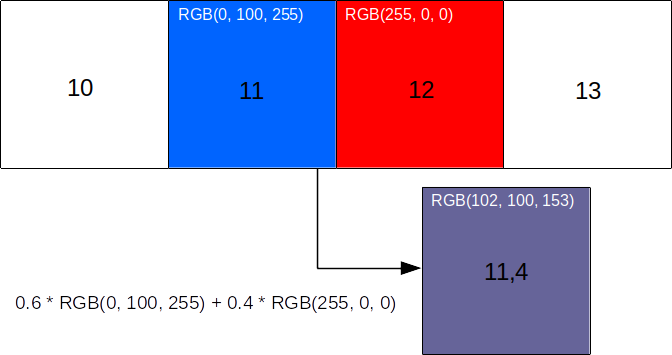
\includegraphics[width=0.85\linewidth]{img/hauptteil/bildverarbeitung/weighted_pixel.png}
		\caption{Gewichtete Pixel für den x-Wert 11,4}
		\label{fig:weighted_pixel}
	\end{figure}
	Die Abbildung \ref{fig:weighted_pixel} zeigt den Vorgang an einem simplen Beispiel für ein Subpixel in einer beliebigen Reihe (y-Wert) mit einem beispielhaften x-Wert von 11,4. Der nähere Pixel (11) fließt mit höheren Gewicht in die resultierende Farbe ein, als der Pixel weiter weg (12). Die y-Werte der Pixel können keinen ungeraden Wert beinhalten, da der Algorithmus zum Finden der Laser-Pixel (Kapitel \ref{chap:erkennen_der_laserlinie}) jede Pixel-Zeile im Bild durchläuft und dort einen neuen x-Wert errechnet.
	
	Dieser komplette Vorgang transformiert genau eine aufgenommene Laserlinie in eine Punktewolke. Um eine ganze Oberfläche zu rekonstruieren muss sich die Position der des Sensors um eine bekannte Länge und Richtung verschieben. Die neu Punktewolke, die aus der neu aufgenommenen Laserlinie resultiert, muss dann entsprechend zu einer Gesamt-Punktewolke ergänzt werden. Um die neuen Punkte korrekt einzufügen, ist es zwingend erforderlich, dass die Bewegung genau bekannt ist. 
	
	\newpage
	
	\subsection{Aufbau / Hardware}
	Für den Lasertiangulationssensor wurde verschiedene Hardware verwendet. Dies soll im Folgendem beschrieben werden. Dabei gibt es zwei verschiedene Abschnitte zu betrachten. Zum einen der Lasertriangulationsensor an sich, der nur in der Lage ist eine Laserlinie in eine Punktewolke umzusetzen. Zum anderen wurde ein Versuchsaufbau angefertigt, um ein Objekt unter dem Sensor entlang zu bewegen. Dabei soll der Sensor regelmäßig eine Punktewolke erstellen. Die zusammengefügte Punktewolke ist dann die Aufnahme der Oberfläche. 
	
		\subsubsection{Hardware-Aufbau des Lasertriangulationssensors}
		Die Hardware des Lasertriangulationssensor besteht grundsätzlich aus einer Kamera und einem Laser.
		
		\begin{figure}[h]
			\centering
			\includegraphics[width=0.7\linewidth]{img/hauptteil/hardware/aufbau_sensor.png}
			\caption{Der Lasertriangulationssensor}
			\label{fig:aufbau_sensor}
		\end{figure}
		Für die Kamera wurde die Basler a2A1920-160ucPRO verwendet. Dabei handelt es sich um eine Industriekamera mit einer Auflösung von 1920 x 1200 Pixeln. Sie ist eine Farbkamera und kann bis zu 164 Bilder pro Sekunde aufnehmen. Die Spezifikationen sind gemäß [basler-cam-spez] angeben. Wichtig ist, dass die Kamera über USB 3.0 angesprochen werden kann. So kann sie über Software auf einem PC oder ähnlichem angesteuert werden. Mit dem Software-Paket Pylon liefert Basler eine eigene Umgebung um die Kamer zu benutzen und einzustellen. Zusätzlich wird mit Pypylon eine Pythonbibliothek gestellt. Diese gilt als Schnittstelle zwischen Kamera und Python. So kann über direkten Python-Code die Kamera eingebunden werden. \newline
		Das zweite Bauteil ist der Laser. Dabei handelt es sich um einen herkömmlichen roten Laser. Der Lichtstrahl des Lasers wird durch diffraktive optische Elemente (DOE) zu einer Linie geformt. Wie in Abb. \ref{fig:aufbau_sensor} gezeigt werden dann Kamera und Laser an eine Halterung in entsprechender Position befestigt. \newline
		Die Kamera hat ein ansteuerbares Output-Signal. Dieses Signal kann genutzt werden, um den Laser direkt anzusprechen. Dabei wird ein MOSFET (Metal Oxide Semiconductor Field-Effect Transistors) verwendet. So kann das Output-Signal angesprochen werden, um über den MOSFET den Strom des Lasers an und aus zu stellen. Es ist damit möglich, für die Kamera selbst einen Ablauf zu definieren, in dem sie zuerst ein Bild aufnimmt, dann den Laser anschaltet und anschließend ein zweites Bild aufnimmt. Zuletzt muss der Laser wieder ausgeschaltet werden. So werden von der Kamera die geforderten Bildpaare aufgenommen. Mit Pypylon können diese Bilden in Python und mit OpenCv weiterverwendet werden.
		
		\subsubsection{Der Versuchsaufbau}
		Das Ziel des Versuchsaufbau ist es Bewegung in die aufgenommene Szene zu bringen. Dabei soll die zurückgelegte Bewegung zwischen den Aufnahmen der Oberfläche bekannt sein. So kann die neue Punktewolke der Laserlinie passend angefügt werden. Andernfalls würde man immer den Querschnitt der aktuellen Oberfläche an der Position des Lasers beobachten. Die einfachste Möglichkeit das zu realisieren ist, wenn sich die Szene in genau eine definierte Richtung mit genauen definierten Abstand bewegt. Dazu wurde eine Linear-Führung benutzt. Diese Funktioniert über ein Schrittmotor und bewegt eine Fläche mit einer linearen Bewegung. Der Schrittmotor kann dabei genau angesprochen werden und das Objekt um in unseren Fall genau einen Millimeter weiter schieben.
		\begin{figure}[h]
			\centering
			\includegraphics[width=0.9\linewidth]{img/hauptteil/hardware/aufbau_linearführung.png}
			\caption{Der Lasertriangulationssensor}
			\label{fig:aufbau_scanner}
		\end{figure}
		Die Linear-Führung stammt aus einem 3D-Drucker. Die Software des Lasertriangulationsensor muss die Steuerung des Schrittmotors ansteuern können. Dieser wird über eine CNC-Steuerung mit Arduino und GRBL-Software angesprochen. Der Arduino ist der Mikrocontroller. Die CNC-Steuerung übernimmt das Ansteuern des Motors. Dazu gibt es ein geeignete Erweiterungsplatinen für einen Arduino, sogenannte CNC-Shields. Damit Arduino und CNC-Shield miteinander kommunizieren können wird die Open-Source-Software GRBL verwendet. So können Befehle des Arduino über GRBL und der CNC-Steuerung für den Schrittmotor lesbar sein.
		\begin{figure}[h]
			\centering
			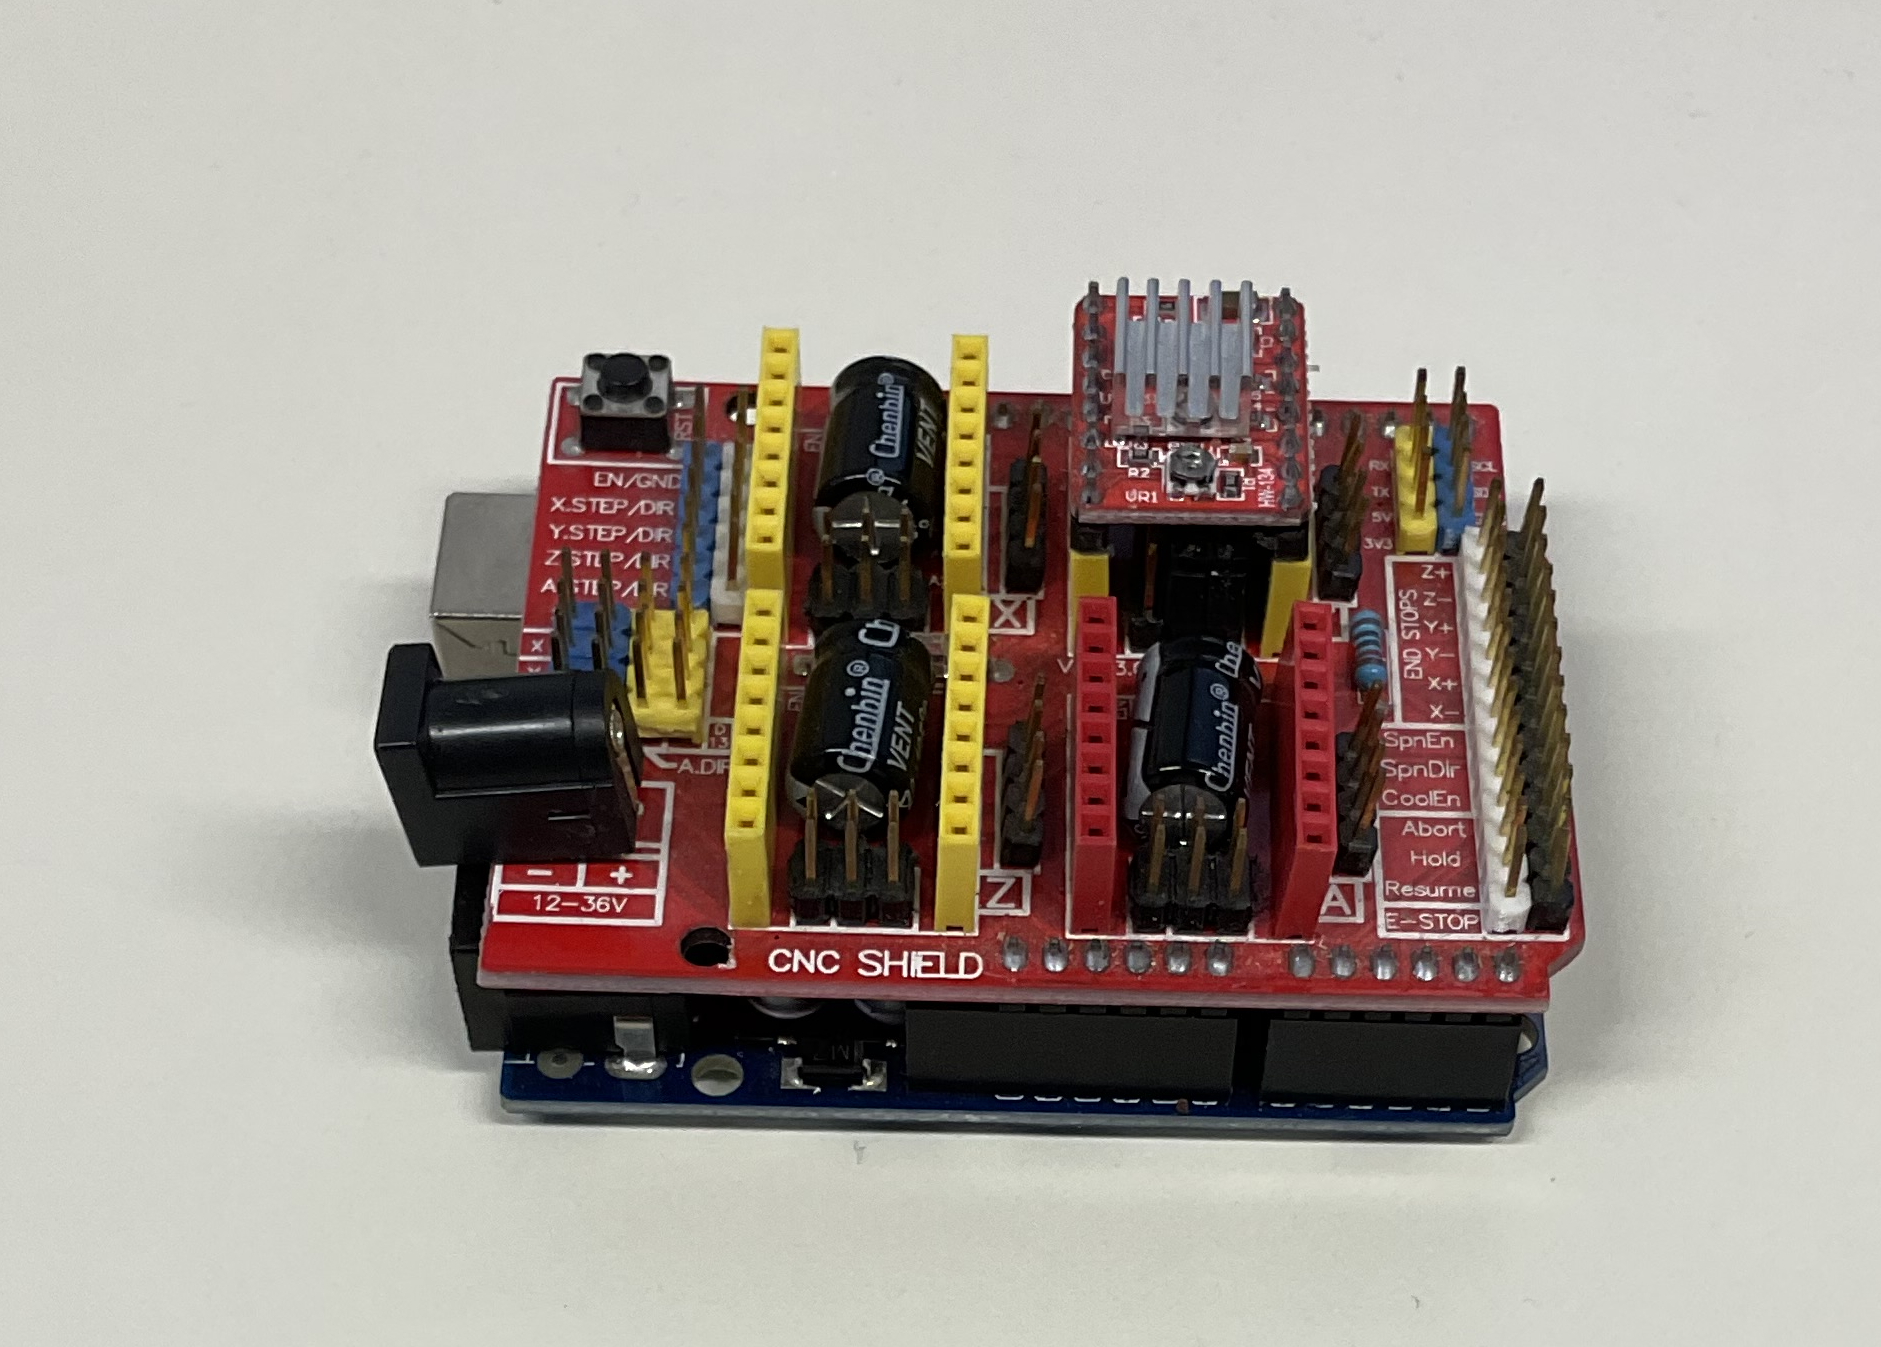
\includegraphics[width=0.45\linewidth]{img/hauptteil/hardware/arduino.png}
			\caption{Arduino mit CNC-Shield}
			\label{fig:arduino}
		\end{figure}
		Mit diesem Aufbau kann über die Bibliothek \textit{serial} in Python eine sogenannte \glqq Serial Connection\grqq{} aufgebaut werden. Damitaab kann direkt über ein USB-Anschluss auch der Motor angesprochen werden. Über die Serial Connection werden dann GRBL-Befehle an den Motor gesendet. Diese sind einfache Befehle wie \glqq Startposition festlegen!\grqq{}, \glqq 1mm bewegen\grqq{} oder \glqq Zur Startposition zurückkehren!\grqq{}.
		
	
	\label{chap:aufbau_hardware}
	
	\newpage
	
	\subsection{Aufbau / Software}
	Die Software des Lasertriangulationssensor gliedert sich in zwei Bereiche. Zum einen wurde eine Python-Bibliothek entwickelt. Diese wurde Objektorientiert mit diversen Klassen, die den Lasertriangulationssensor repräsentieren entwickelt. Grundlegende Aufgabe der Python-Bibliothek sind die elementaren Berechnungen, um eine Punktewolke aus einem Bild-Paar zu erhalten. Das bedeutet, dass ein Konstrukt erstellt werden kann, welches Kalibriert werden kann und darauf folgend Punktewolken liefert. \newline
	Der andere große Bereich ist die Umsetzung in ROS2. ROS2 liefert das Betriebssystem des Scanners. Alle verschiedenen Elemente sollen zu einem Gesamtprodukt zusammengefügt werden. Dazu gehört die Ansteuerung der Kamera und des Lasers. Schwerpunkt ist auch die Kommunikation zwischen einzelnen Elementen. Beispiele sind dabei das Aufnehmen der Bilder für die Kalibrierung oder das Erstellen der Punktewolke und die Weiterleitung an die entsprechenden Methoden aus den Klassen der Python-Bibliothek.
		\subsubsection{Python (Bibliothek)}
		Die Python-Bibliothek besteht grundlegend aus vier Klassen. Die Scanner-, Kamera-, Laser-, und LaserLine-Klasse. Dabei ist die Scanner-Klasse die volle Repräsentation des Lasertriangulationssensors, die in ROS2 eingebunden wird.
		
		\begin{figure}[h]
			\centering
			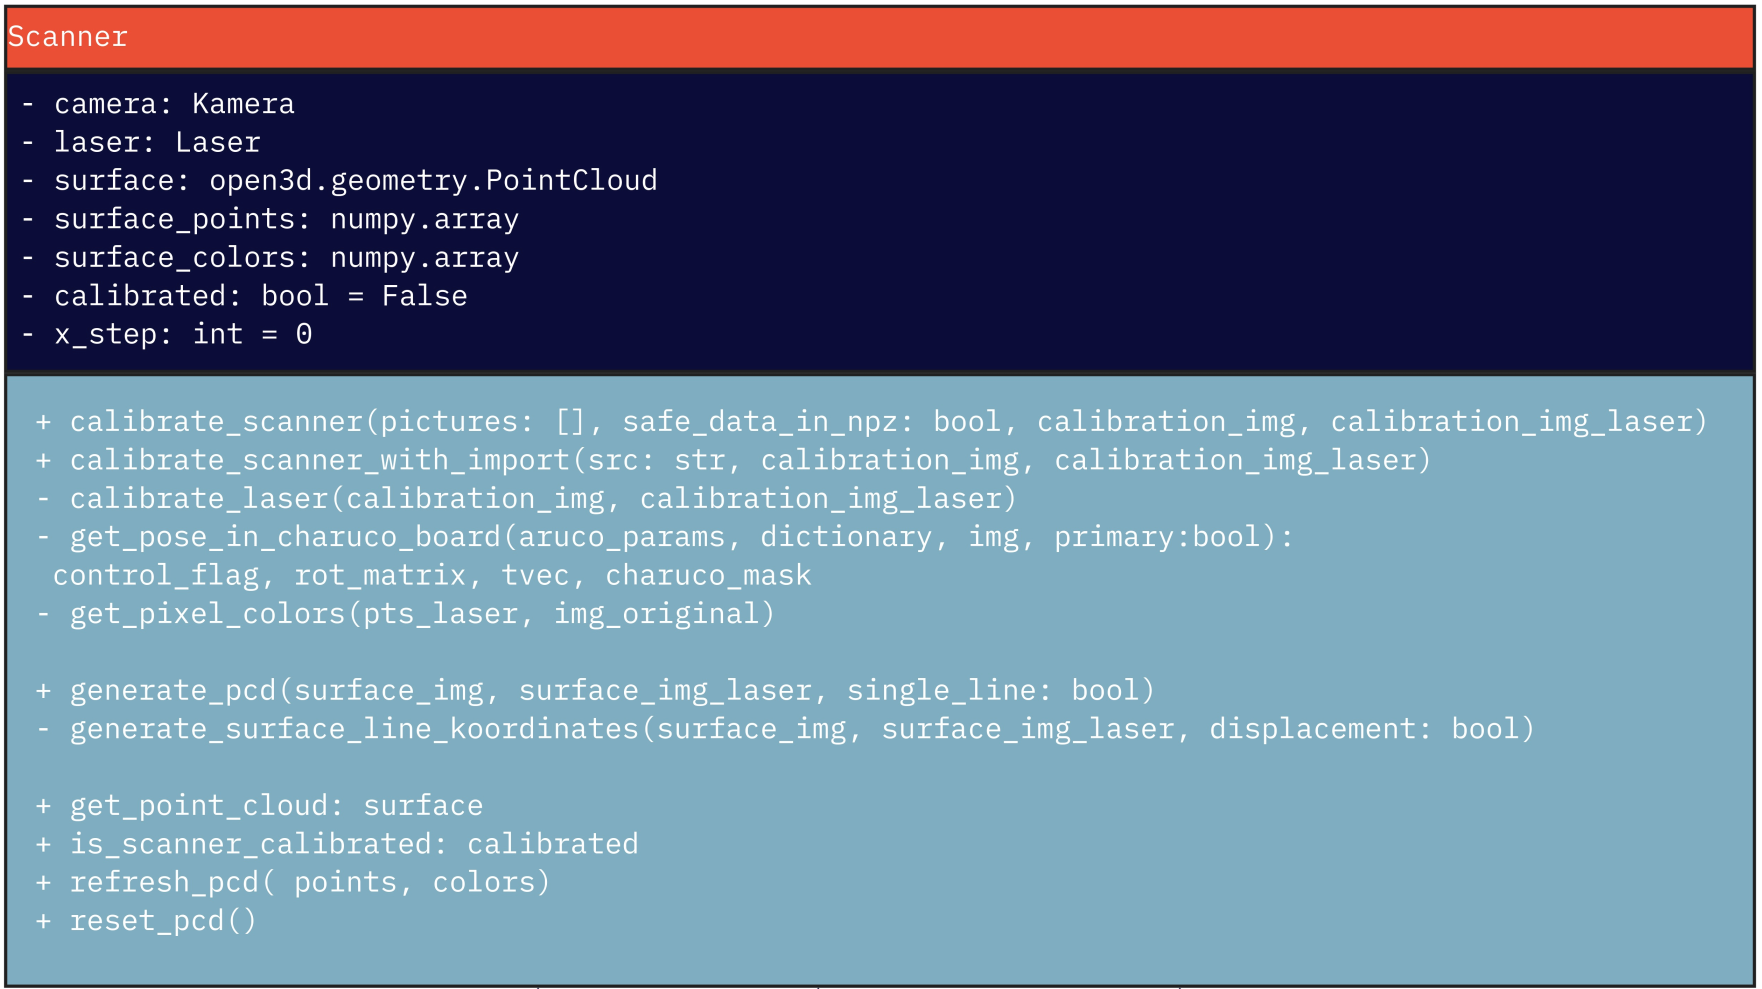
\includegraphics[width=0.85\linewidth]{img/hauptteil/software/Scanner_UML.png}
			\caption{Die Scanner-Klasse als UML-Diagramm}
			\label{fig:scanner_uml}
		\end{figure}
		Der Scanner beschreibt den Lasertriangulationssensor. Er besitzt eine Kamera und einen Laser. Zusätzlich wird als Variable die Punktewolke der Oberfläche und auch direkt deren Punkte und Farben abgespeichert. Hinzu kommt ein Boolean-Flag um zu kennzeichnen, ob der Scanner kalibriert ist. Der xStep ist für den Versuchsaufbau wichtig. Über die Liniarführung wird das Objekt in x-Richung unter dem Sensor durch bewegt. Die jeweiligen Millimeter-Schritte müssen entsprechend einbezogen werden. Dazu wird diese Variable genutzt. \newline
		Zusätzlich stellt die Scanner-Klasse die grundlegenden Methoden, die die Funktionalität des Triangulationssensors wieder spiegel, zur Verfügung. Diese umfassen zum einen das komplette kalibrieren des Scanners. Dazu wird eine Liste von Bildern für die intrinsische Kalibrierung und ein Bildpaar des ChArUco-Boards für die extrinsische Kalibrierung benötigt. Hinzu kommt eine abgewandelte Version der Kalibrier-Methode, in der die intrinsische Kalibrierung durch das Importieren der Kameradaten ersetzt wird. Hinzu kommt die Methode zum Erstellen einer Punktewolke. Sie bekommt ein entsprechendes Bildpaar von der Oberfläche übergeben und errechnet die Punktewolke. Wenn der Scanner sich gerade in einem Scanvorgang befindet wird die neue Punktewolke entsprechend an die gesamte Punktewolke angehängt. Die Scanner-Klasse besitzt zusätzlich noch Hilfsmethoden die Zugriff von außen auf den Scanner Status und die Punktewolke geben oder die Punktewolke selbst erneuern oder aktualisieren.
		
		\begin{figure}[h]
			\centering
			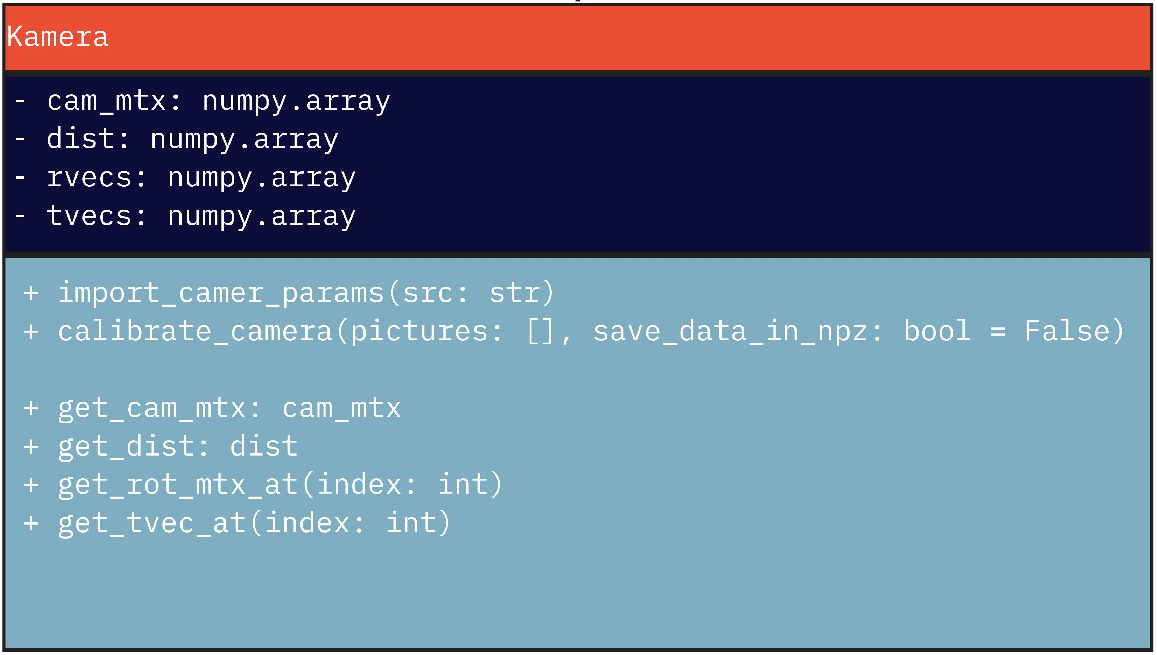
\includegraphics[width=0.7\linewidth]{img/hauptteil/software/Kamera_UML.png}
			\caption{Die Kamera-Klasse als UML-Diagramm}
			\label{fig:kamera_uml}
		\end{figure}
		Die Kamera selbst besitzt auch eine Repräsentation in Form einer Klasse. Diese Klasse fungiert als Speicher für die Kameradaten. Gespeichert werden die Kamera-Matrix die Distortion-Koeffizienten und die Rotationsmatrizen sowie die Translationsvektoren der Bilder von der intrinsischen Kalibrierung. Also alle Daten, die aus der intrinsische Kalibrierung hervorgehen. Hierbei ist wichtig hervorzuheben, dass die Klasse keine Bilder aufnehmen kann bzw kein Zugriff auf die tatsächliche Kamera im Triangulationssensor hat. Sie is lediglich für das Ablegen der Daten und die intrinsische Kalibrierung zuständig.
		\newpage
		\begin{figure}[h]
			\centering
			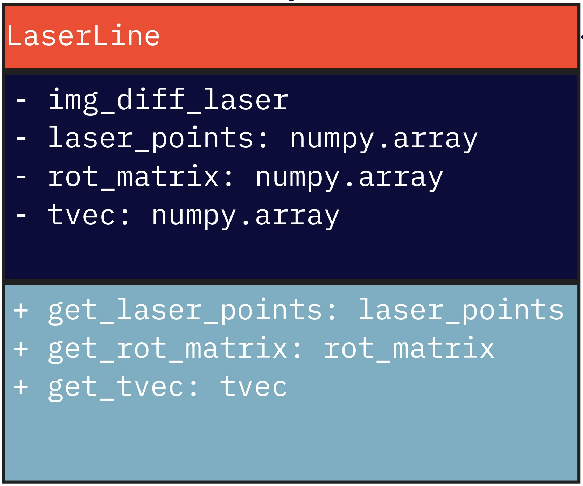
\includegraphics[width=0.35\linewidth]{img/hauptteil/software/LaserLine_UML.png}
			\caption{Die LaserLine-Klasse als UML-Diagramm}
			\label{fig:laser_line_uml}
		\end{figure}
		Die Klasse LaserLine beschreibt eine aufgenommene Laserlinie. Information die dafür als Variablen gespeichert werden sind das Differenz-Bild, die errechneten 3D-Punkte der Linie und die entsprechende Rotation und Translation zu dem Weltkoordinatensystem, in dem sich die Laserlinie befindet. Zum initialisieren der LaserLine-Klasse wird das aufgenommene Bildpaar und die Rotation und Translation zu dem jeweiligen Weltkoordinatensystem benötigt. Die Klasse errechnet dann noch im Konstruktor die Bild-Differenz und die Laserlinienpunkte.
		
		\begin{figure}[h]
			\centering
			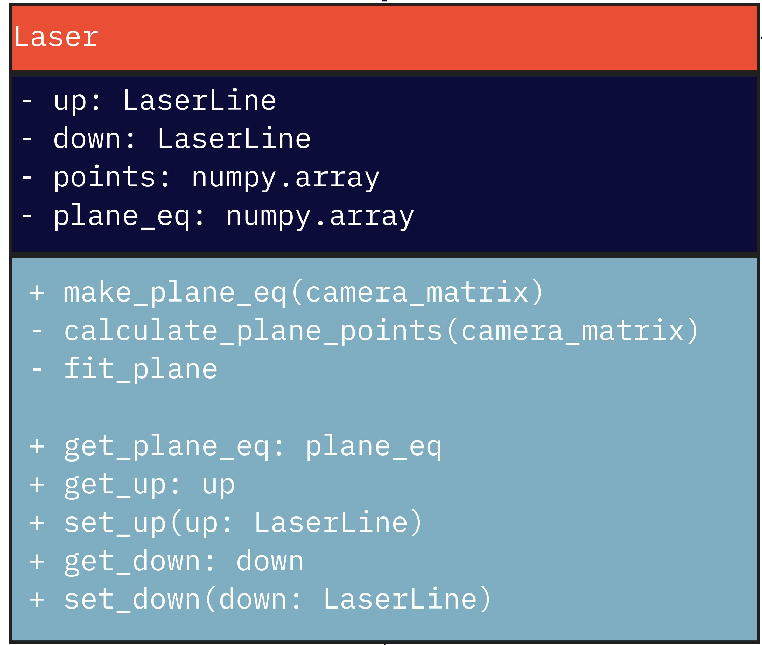
\includegraphics[width=0.35\linewidth]{img/hauptteil/software/Laser_UML.png}
			\caption{Die Laser-Klasse als UML-Diagramm}
			\label{fig:laser_uml}
		\end{figure}
		So wie die Kamera-Klasse die Daten der intrinsischen Kalibrierung beinhaltet, beinhaltet die Laser-Klasse die Daten der extrinsischen Kalibrierung. Dazu benötigt sie zwei Laserlinien der Klasse LaserLine, die zur Unterscheidung als \glqq oben\grqq{} und \glqq unten\grqq{} definiert sind. Aus diesen kann die Ebenengleichung bestimmt werden. Dazu wird eine eigene Methode bereitgestellt in der erst die Punkte in ein einheitliches Koordinatensystem zusammengefasst und dann eine Ebene an die Punkte gefittet wird. Die vereinheitlichten Punkte und die Ebenengleichung werden von der Klasse gespeichert.
		\newpage
		\begin{figure}[h]
			\centering
			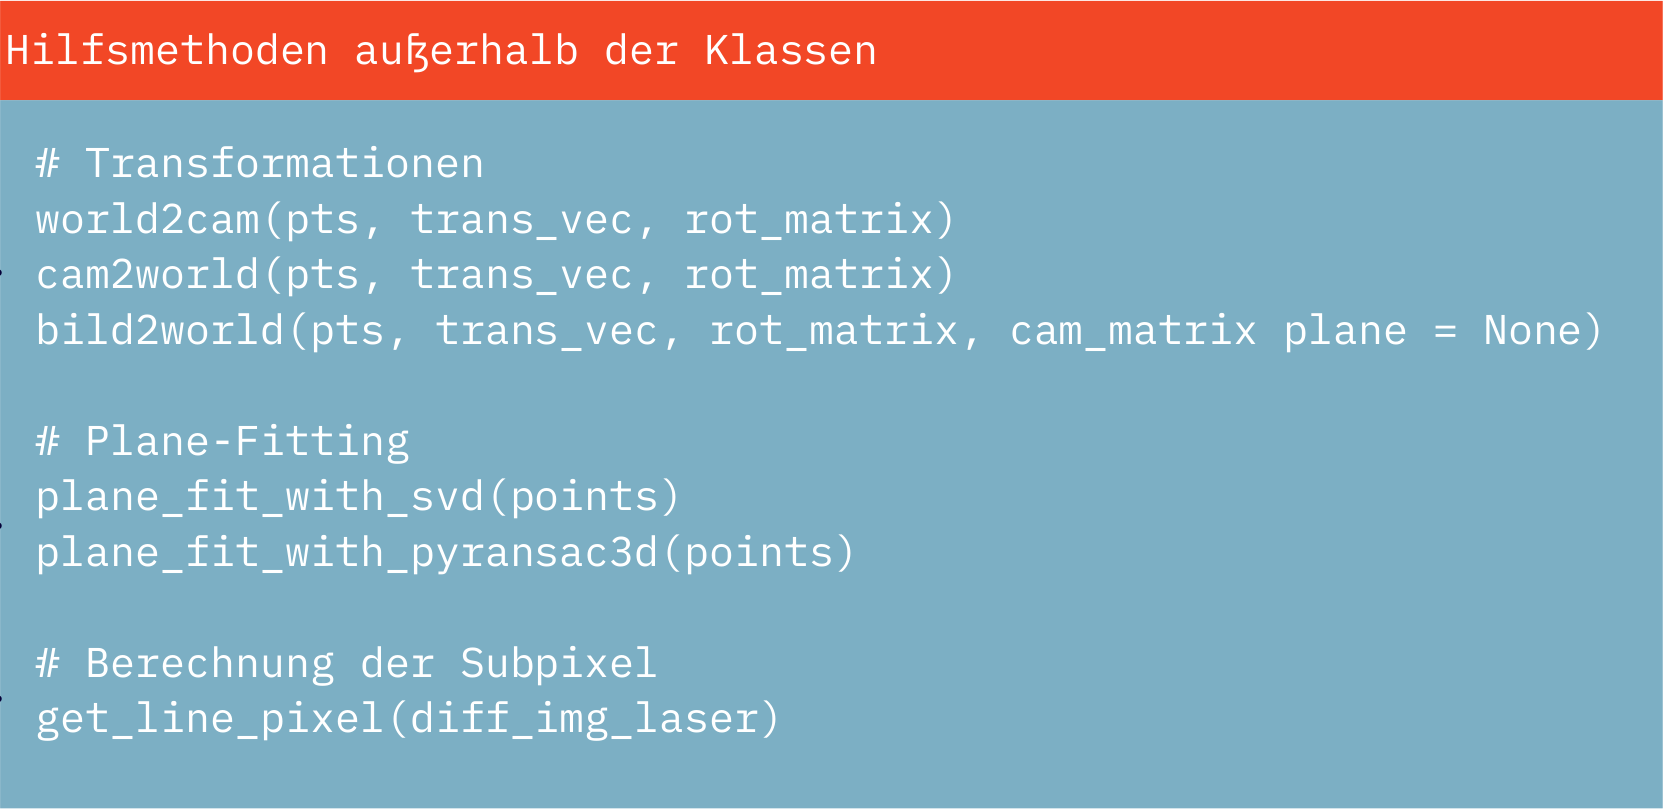
\includegraphics[width=0.7\linewidth]{img/hauptteil/software/Hilfsmethoden_UML.png}
			\caption{Die Hilfsmethoden ohne Zugehörigkeit zu einer Klasse}
			\label{fig:hilfsmethoden_uml}
		\end{figure}
		Zusätzlich zu den vier beschriebenen Klassen gibt es Hilfsmethoden, die nicht konkret zu einer Klasse gehören. Das bedeutet, dass sie nicht nur von einer Klasse benutzt werden, sondern von verschiedenen Klassen an verschiedenen Stellen aufgerufen werden. Diese Methoden umfassen die Transformationen zwischen den Koordinatensystemen, die Methoden für das Plane-Fitting und die Berechnung der Subpixel aus einem Differenz-Bild.
		
		Die gesamte Darstellung des UML-Diagramm befindet sich im Anhang unter Abbildung \ref{anhang-a}.
		
		\subsubsection{ROS2}
		
		Übergeordnet über der Python-Bibliothek befindet sich die ROS2-Implementierung, mit der letztendlich der Triangulationssensor bedient wird. Mit ROS2 erstellt man sogenannte \textbf{Nodes}, die verschiedene Möglichkeiten bereitstellen miteinander zu kommunizieren. Dazu gehören zum einen \textbf{Services}. Services sind am ehesten mit Methoden einer Klasse zu vergleichen, wobei dann die Nodes eine Klasse darstellen. Eine Node stellt ein Service bereit. Dieser kann aufgerufen werden und man erhält eine Antwort zurück. Der Triangulationssensor selbst ist auch über Nodes umgesetzt. Dabei sind die beiden ausschlaggebenden Nodes die Scanner-Node und die Kamera-Node. Die Scanner-Node enthält die vorgestellte Python-Bibliothek und damit eine Instanz von der Scanner-Klasse. Die Instanzen von der Scanner-Klasse selbst, also der Laser und die Kamera sind nach Initialisierung noch nicht mit Daten gefüllt. Das liegt daran, dass die Kalibrierung noch nicht stattgefunden hat. Dazu gibt es die Kamera-Node, die nun konkrete Bilder liefern kann. Die Kamera-Node hat Zugriff auf die Pypylon-Bibliothek [pypylon] und damit auf die Repräsentation der Basler-Kamera. Die Node beinhaltet eine Funktion, die das gewünschte Bildpaar liefert. Da der Linienlaser selbst über den Output der Kamera gesteuert wird, kann dieser auch direkt in der Kamera-Node angesprochen werden. So stellt die Kamera ein Service bereit, der ein Bildpaar aufnimmt und dieses an den Scanner weiterleiten kann. Genauso stellt sie einen Service bereit, der mehrere Bilder aufnimmt und diese als Liste weiterleitet. Damit ist auch für die intrinsische Kalibrierung gesorgt. \newline
		Diese Kommunikation funktioniert in ROS2 über \textbf{Topics}. Topics beschreiben eine Nachricht. Eine Node hat die Möglichkeit eine Nachricht über ein gewähltes Topic zu veröffentlichen (publish). Ebenfalls gibt es die Möglichkeit , dass eine Node Nachrichten über ein gewähltes Topic empfängt (subscribe). Der Service hier nimmt ein Bildpaar auf und veröffentlicht es über das jeweilige Topic. Was die Scanner-Node beim Eintreffen der Bilder macht, ist für den Service selbst nicht mehr von Belangen.\newline
		In der Kommunikation muss zusätzlich festgehalten werden, welchen Datentyp die Nachricht bzw. das Topic verwenden soll. In ROS2 wird das über einen \textbf{Message}-Type realisiert. Hierbei kann man selbst eine Message erstellen oder man benutzt Vorgefertigte, die von ROS2 bereitgestellt werden. Für ein Bild gibt es einen vorgefertigten Message-Type. Da jedoch zwei Bilder auf einmal geschickt werden sollen, wurde hier ein eigener Typ (img\_pair.msg) erstellt. Ähnlich verhält es sich bei dem Schicken der Kalibrierungsbilder für die intrinsische Kalibrierung. Hier wird ein Message-Type erstellt, der eine Liste an Bildern beinhaltet (cam\_calib\_imgs.msg). Die Kamera nimmt demnach bei einem Aufruf des Services die Bilder auf und veröffentlicht sie über das jeweilige Topic. Der Scanner ist ein Subscriber zu diesem Topic und empfängt sie. Dabei wird in der Node eine Callback-Function aufgerufen, die auf dieses Empfangen reagiert. Der Scanner selbst speichert die für die Kalibrierung gesendeten Bild erst einmal nur ab. Zusätzlich hat ein Service in ROS2 dei Möglichkeit ein Feedback zurückzugeben. Diese Möglichkeit wird hier genutzt, damit die Kamera zeigen kann, dass die Bilder erfolgreich aufgenommen und veröffentlicht wurden.\newline
		Die Scanner-Node stellt einen eigenen Service bereit, der den Scanner Kalibriert. Dazu werden die Methoden, die die Scanner-Klasse bereitstellt genutzt. Überprüft wird hierbei, ob dem Scanner schon die benötigten Bilder bereitstehen. Falls das nicht der Fall ist, wird über die Antwort des Services darauf hingewiesen und der Aufruf des Services schlägt fehl. Andernfalls kann die Node den Scanner Kalibrieren und ein Scan kann gestartet werden. \newline
		In der ROS2-Implementierung gibt es noch zwei weitere Nodes. Zum einen wird ein Empfänger gebraucht, der entsprechende Ergebnisse des Scanners auch empfangen und benutzen kann. In diesem Fall werden von Scanner Punktewolken veröffentlicht. Das geschieht auch wieder über ein Topic. Dabei ist der Message-Type des Topics ein von ROS2 vorgefertigter Typ, der Punktewolken beinhaltet. Benötigt demnach wieder eine Node, die ein Subscriber des Punktewolken-Topic ist. Dazu wird \textbf{Rviz2} benutzt. Rviz2 ist ein von ROS2 bereitgestellten Paket und dient zur Visualisierung. Die Funktionalität von Rviz2 ist sehr weitgehend. Wichtig für den Lasertriangulationssensor ist, dass es Rviz2 möglich Subscriber von dem Punktewolken-Topic zu sein. Die Empfangenen Punktewolken können hier dargestellt und dynamisch beobachtet werden. \newline
		Die vierte Instanz, die benötigt wird, sind sogenannte Clients. Es wurde schon öfters von Services und dem Aufrufen eines Service geredet. In ROS2 wird dafür ebenfalls eine Node benötigt, die den jeweiligen Service aufruft und das entsprechende Feedback erhält. In der Anlage unter \ref{anhang-b} befindet sich eine Grafik, die die Nodes und ihre Kommunikationswege darstellt. Die Client-Node wird dort als eine einzelne Node zusammengefasst. Intern wird für jeden Aufruf eines Services jedoch eine eigene individuelle Node generiert. Da diese allerdings alle den selben Zweck folgen, den bestimmten Service aufrufen und das Feedback ausgeben, wurden sie hier als eine einzelne Node zusammengefasst. Als Nutzer startet man die jeweiligen Clients, um das gewollte System zu starten. Voraussetzung dabei ist, dass die Service-Nodes, hier der Scanner und die Kamera, ebenfalls gestartet und aktiv sind. Diese werden genauso, wie ein Client gestartet, nur dass sie selbst nicht aktiv etwas tun, es sei denn der Service, den sie bereit stellen wird aufgerufen oder ein Topic von dem sie Subscriber sind wird veröffentlicht. Sie warten also auf eine Interaktion. Die Client-Nodes sind dabei die Akteure, die eine Interaktion hervorrufen. Das Starten der Nodes ist in ROS2 über Konsolen-Skripts umgesetzt. Die wichtigen Skripts, die von einer gewissen Aktionskette gefolgt sind, sollen im Folgenden beschrieben werden. In \ref{anhang-b} wurden diese Skripts als Funktionen (Functions) benannt, da sie nicht einfach nur eine Node starten, sondern im ganzen System etwas zum Laufen bringen.
		
		$\underline{Vorgang\;bei\;der\;Kalibrierung\;des\;Lasertriangulationssensors}$
		
		Die jetzt beschriebenen Vorgänge sind im Anhang unter \ref{anhang-c} in einem Sequenz-Diagramm visualisiert. \newline
		Der Scanner brauch für eine Kalibrierung Bilder für die intrinsische und für die extrinsische Kalibrierung. Da das sich die Szene der Bilder ändert, findet zwischen den Kameraaufnahmen keine Automatisierung statt. Das bedeutet, dass manuell zuerst die Bilder-Liste der intrinsischen Kalibrierung und das Bild-Paar der extrinsischen Kalibrierung von der Kamera geschickt werden muss, bevor die Kalibrierung selbst erfolgen kann. Welche Aufnahme zuerst erfolgt, ist dabei nicht wichtig. In \ref{anhang-c} wird zuerst die Funktion \textbf{intr\_calib\_imgs} aufgerufen. Diese startet ein Client, der den Service der Kamera \textbf{send\_cam\_calib\_imgs} aufruft. Die Kamera-Node benutzt daraufhin ihre Funktion zum Aufnehmen der Kalibrierbilder. Der Benutzer muss dann für jedes Bild das Schachbrett in einer anderen Position vor die Kamera halten. Die Kamera-Node veröffentlicht die Bild-Liste und schickt ein positives Feedback an den Client zurück. Der Client gibt das Feedback in der Konsole aus und ist damit fertig. Die Node hört somit auf zu existieren. Der Scanner reagiert auf das veröffentlichen der Bilder und speichert sie ab. \newline
		Der selbe Vorgang passiert bei der Funktion \textbf{extr\_calib\_imgs}. Der Unterschied besteht darin, dass der Client ein anderen Service (\textbf{send\_laser\_calib\_imgs}) aufruft. Der Benutzer muss hier das Kalibrier-Brett mit dem ChArUco-Board vor die Kamera halten. \newline
		Der Scanner ist nun im Besitzt der benötigten Bilder. Mit der Funktion \textbf{calibrate} wird ein Client gestartet, der den Service \textbf{calibrate\_laser} der Scanner-Node aufruft. Das veranlasst die Scanner-Node dazu, die Funktion \textit{calibrate\_scanner()} der internen Scanner-Klasse aufzurufen. Für die Visualisierung und zum Überprüfen erstellt die Scanner-Node eine Punktewolke, die die Laserebene darstellt und veröffentlicht sie über ein Topic. Über Rviz2 kann dann das Ergebnis der Kalibrierung angesehen werden.
		
		$\underline{Vorgang\;des\;Scannabblauf}$
		
		Die jetzt beschriebenen Vorgänge sind im Anhang unter \ref{anhang-d} in einem Sequenz-Diagramm visualisiert. \newline
		Nachdem der Scanner kalibriert ist, kann ein Scann-Vorgang, zugeschnitten auf den Versuchsaufbau vorgenommen werden. Hierbei wird kein konkreter Service der Scanner-Node benutzt. Die Scanner-Node weiß viel mehr, dass das gesendete Bild-Paar von der Oberfläche aufgenommen wurde und eine Punktewolke errechnet werden soll. Das verwendete Topic (\textit{ImgPair}) hat einen Message-Type, der zwei Bilder beinhaltet. Dieser kann somit sowohl für die extrinsische Kalibrierung, als auch für ein Bildpaar von der Oberfläche genutzt werden. Hier wurde ein Boolean-Flag eingebaut, der zeigt, ob das Bild-Paar für die Kalibrierung oder zur Oberflächenrekonstruktion benutzt werden soll. Somit weiß die Scanner-Node genau, wie sie weiterzuarbeiten hat. Falls die Scanner-Node ein Bildpaar zur Oberflächenrekonstruktion erhält, aber nicht kalibriert ist, wird der Fehlerfall mit einer entsprechenden Warnung behandelt. \newline
		Die Funktion \textbf{start\_scan} starten einen Client, der zum Anfang der Scanner-Node über das Topic \textbf{ScannerStatus} signalisiert, dass sie sich jetzt im laufenden Scann befindet. Der Scann startet damit, dass der Service \textbf{send\_img\_pair\_surface} der Kamera aufgerufen wird. Die Kamera nimmt ein Bild-Paar auf und veröffentlicht es. Der Scanner reagiert darauf, in dem er das Bildpaar in eine Punktewolke umsetzt. Diese wird dann ebenfalls veröffentlicht und in Rviz2 dargestellt. Mit dem Senden des Bild-Paares schickt die Kamera ein positives Feedback an den Client zurück. Der Client signalisiert dann der Serial-Connection über die Sprache Grbl, dass sich die Linearführung um einen Millimeter bewegen soll. Danach wiederholt sich der Vorgang mit dem Aufrufen des Services der Kamera. Dabei bestimmt der Client wie oft sich der Vorgang wiederholt. Im Versuchsaufbau bewegt sich die Linear-Führung 290mm, somit wird der Vorgang 290 mal wiederholt. Die Scanner-Node selbst zählt auch mit, wie oft ein Bild-Paar veröffentlicht wurde und rechnet die Verschiebung mit ein. Die aktualisierte Punktewolke wird dabei immer selbst neu veröffentlicht und in Rviz2 aktualisiert. \newline
		Nachdem alle Wiederholungen durchgeführt wurden signalisiert der Client der Scanner-Node, dass der Scann fertig ist. Daraufhin wird der Scanner die finale Punktewolke in einem (.ply)-File speichern und dann die intern gespeicherte Punktewolke auf null setzten. Damit ist er bereit führ einen erneuten Scann und behält seine Kalibrierung bei.
		
		\newpage
		
		
	\subsection{Qualitative Ergebnisse}\label{chap:qual_ergeb}
	
	In diesem Abschnitt sollen qualitative Ergebnisse von einem Scann-Vorgang gezeigt werden.
	
	\begin{figure}[h]
		\centering
		\subfloat[]{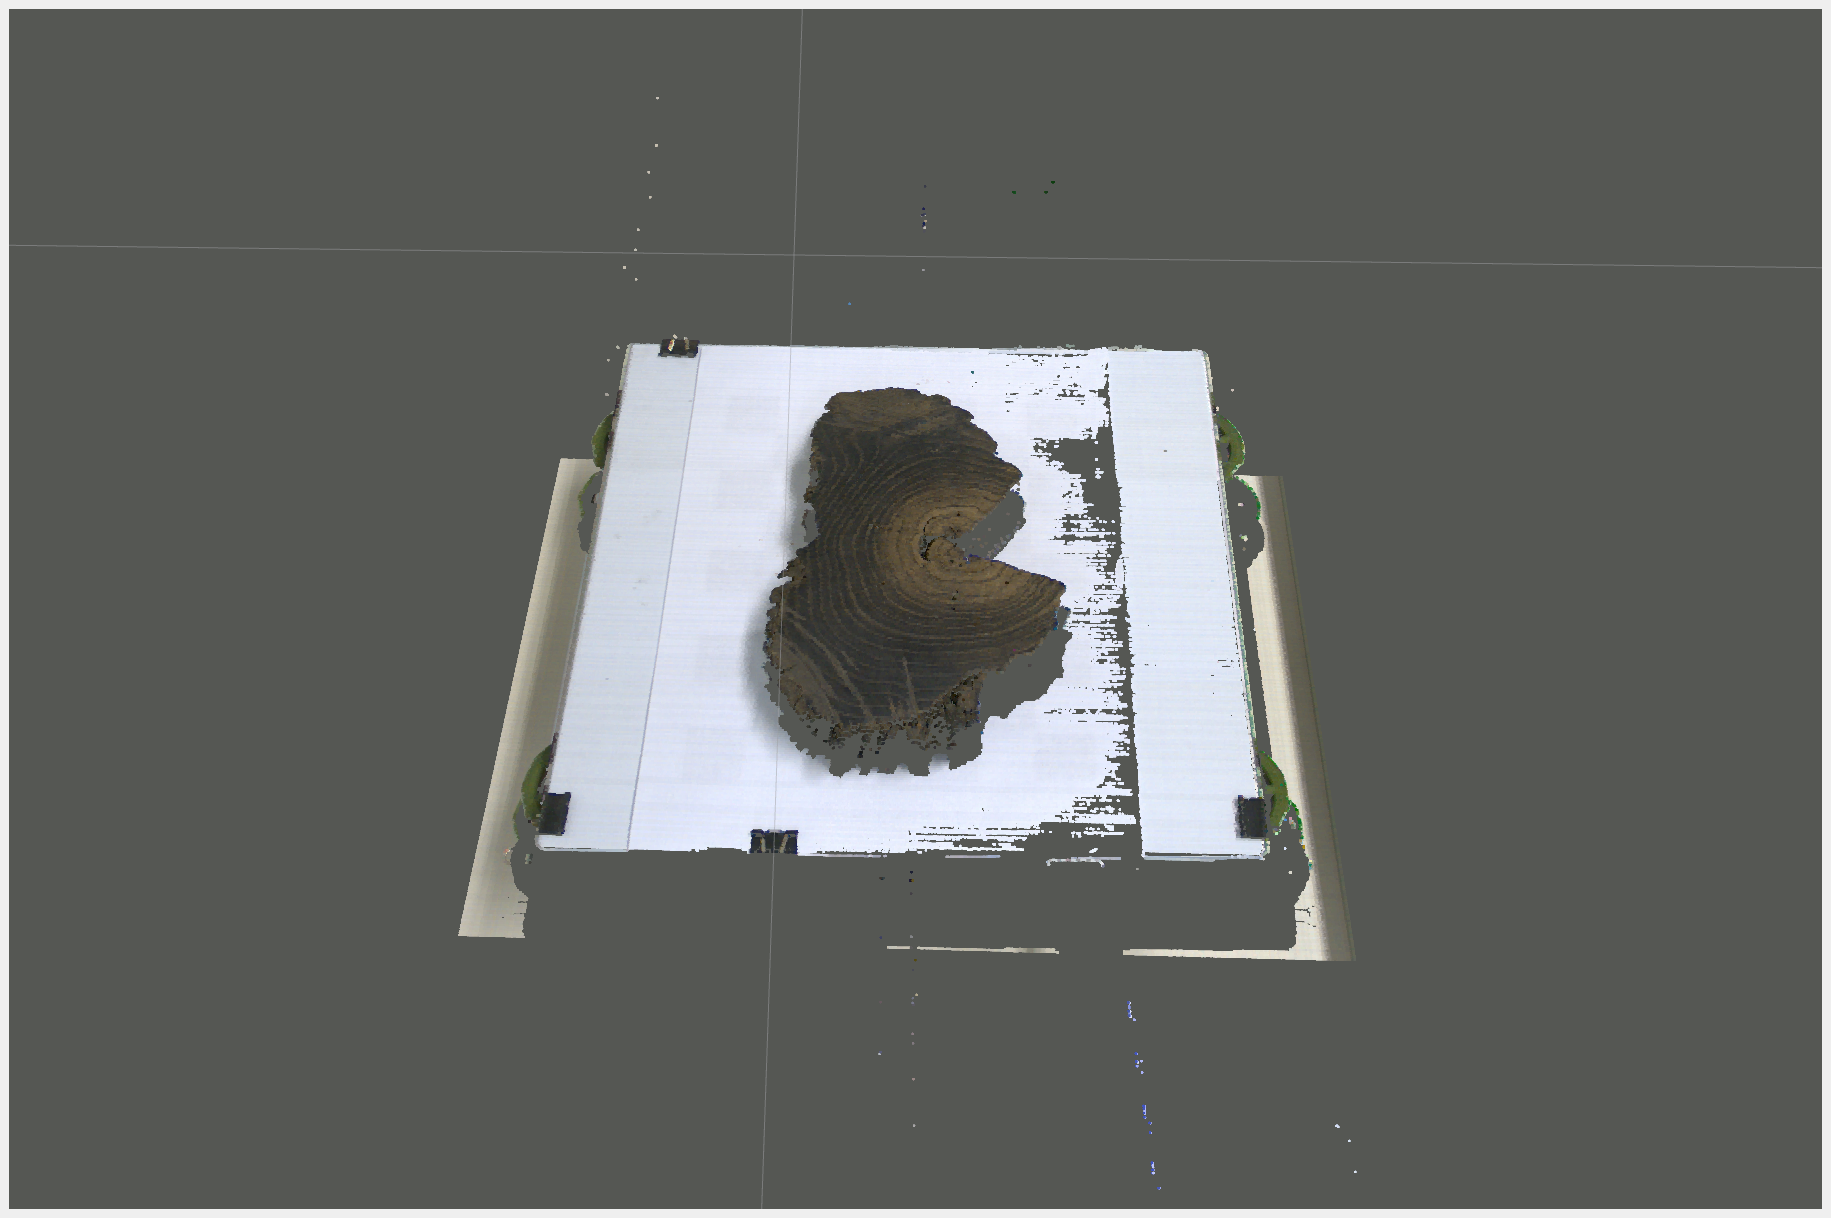
\includegraphics[width=0.49\linewidth]{img/hauptteil/scan-imgs/scan_img_0.png}
			\label{subfig:scan_0}}
		\subfloat[]{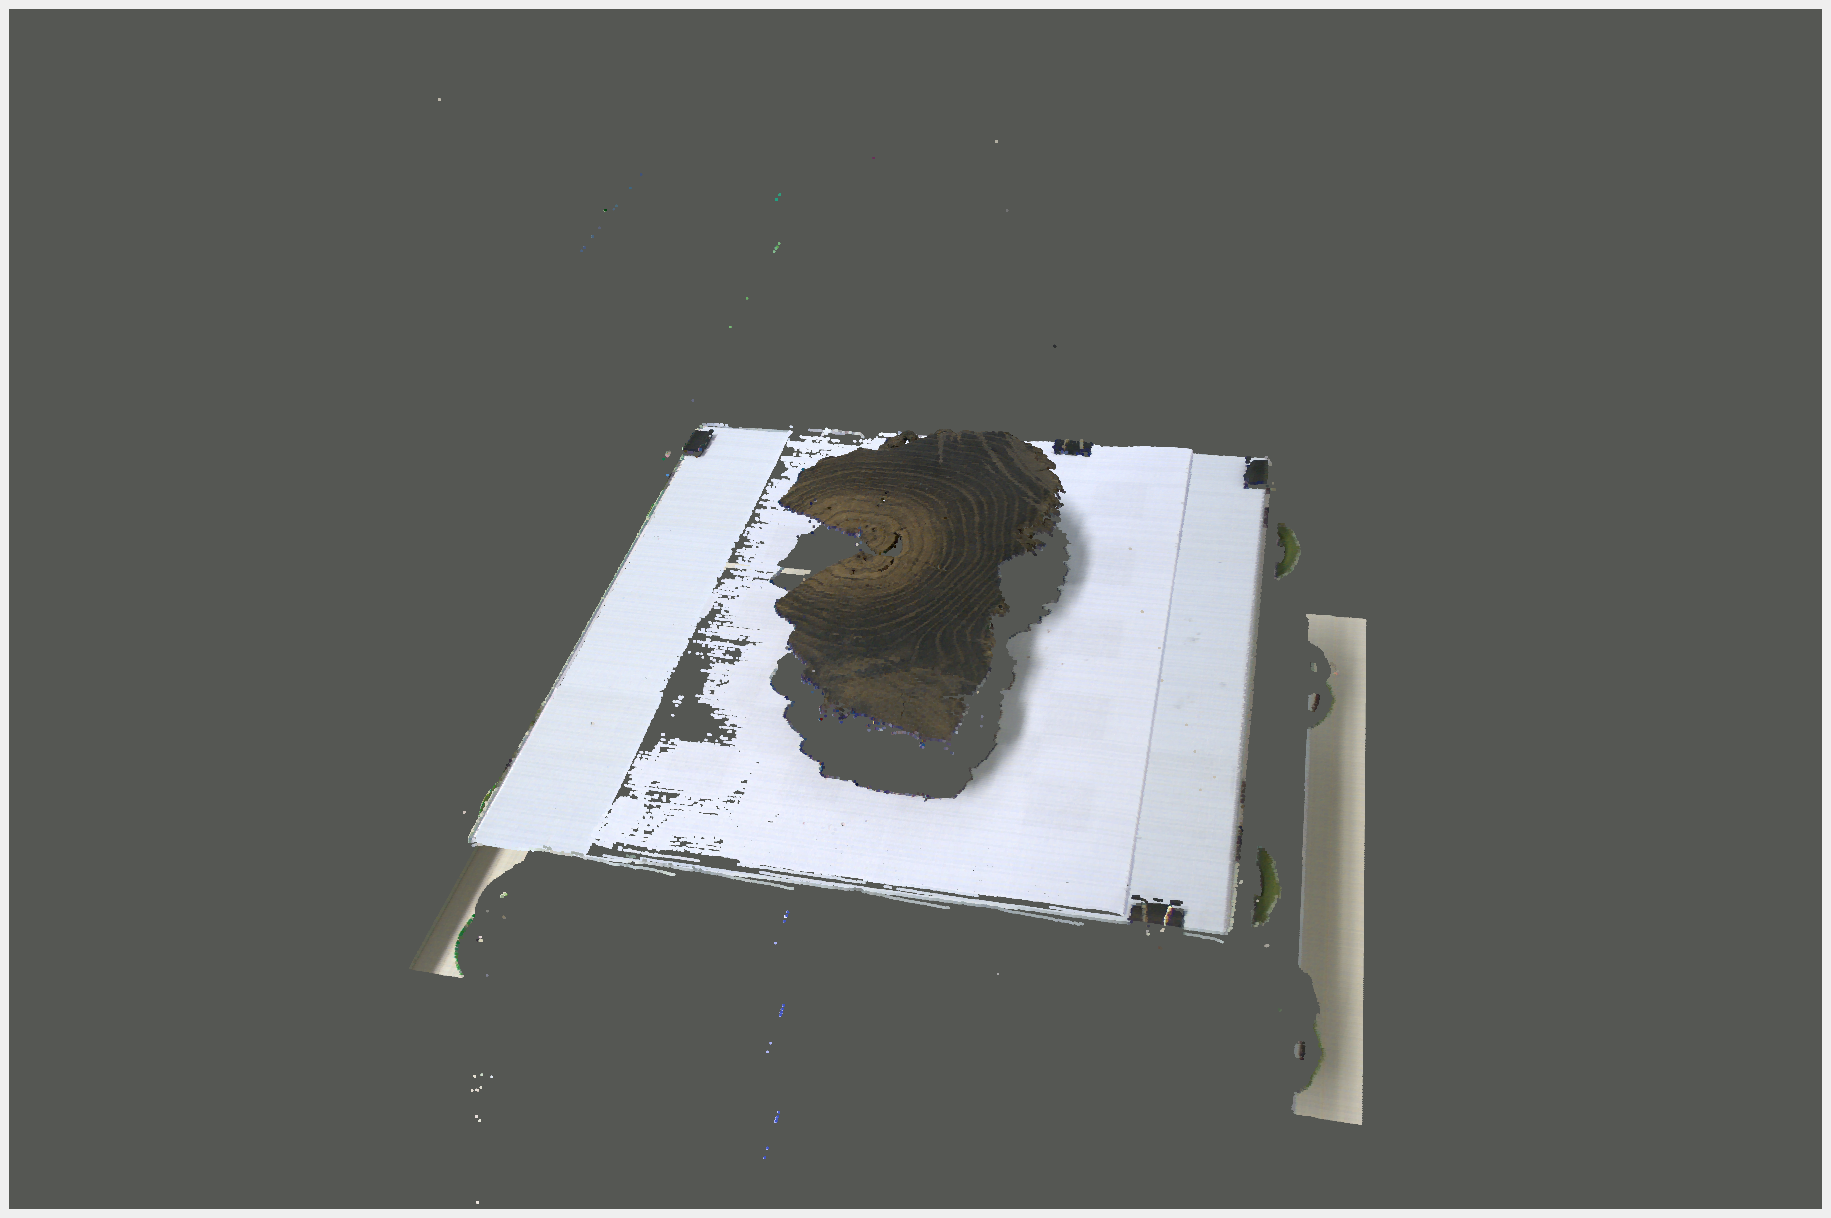
\includegraphics[width=0.49\linewidth]{img/hauptteil/scan-imgs/scan_img_1.png}
			\label{subfig:scan_1}} \\
		\subfloat[]{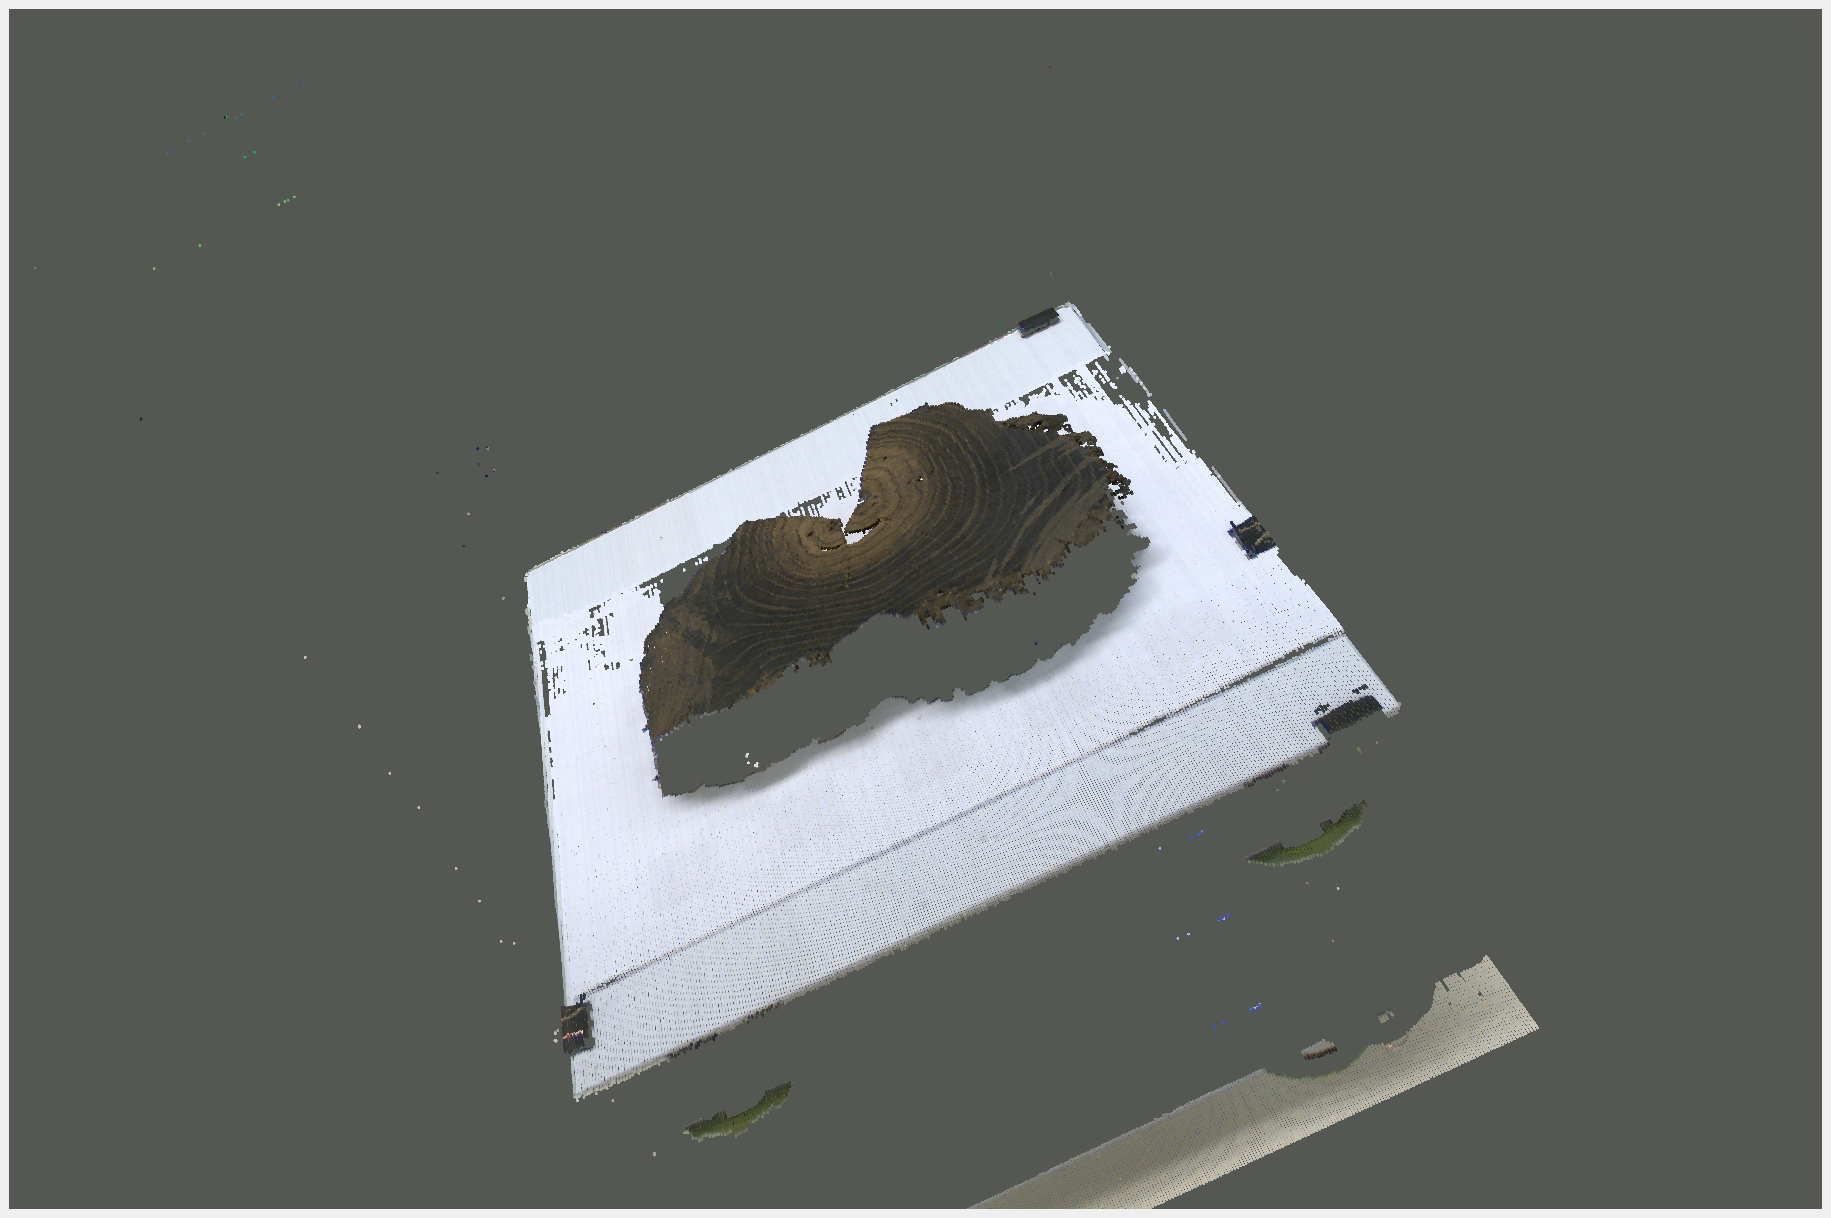
\includegraphics[width=0.49\linewidth]{img/hauptteil/scan-imgs/scan_img_2.png}
			\label{subfig:scan_2}}
		\subfloat[]{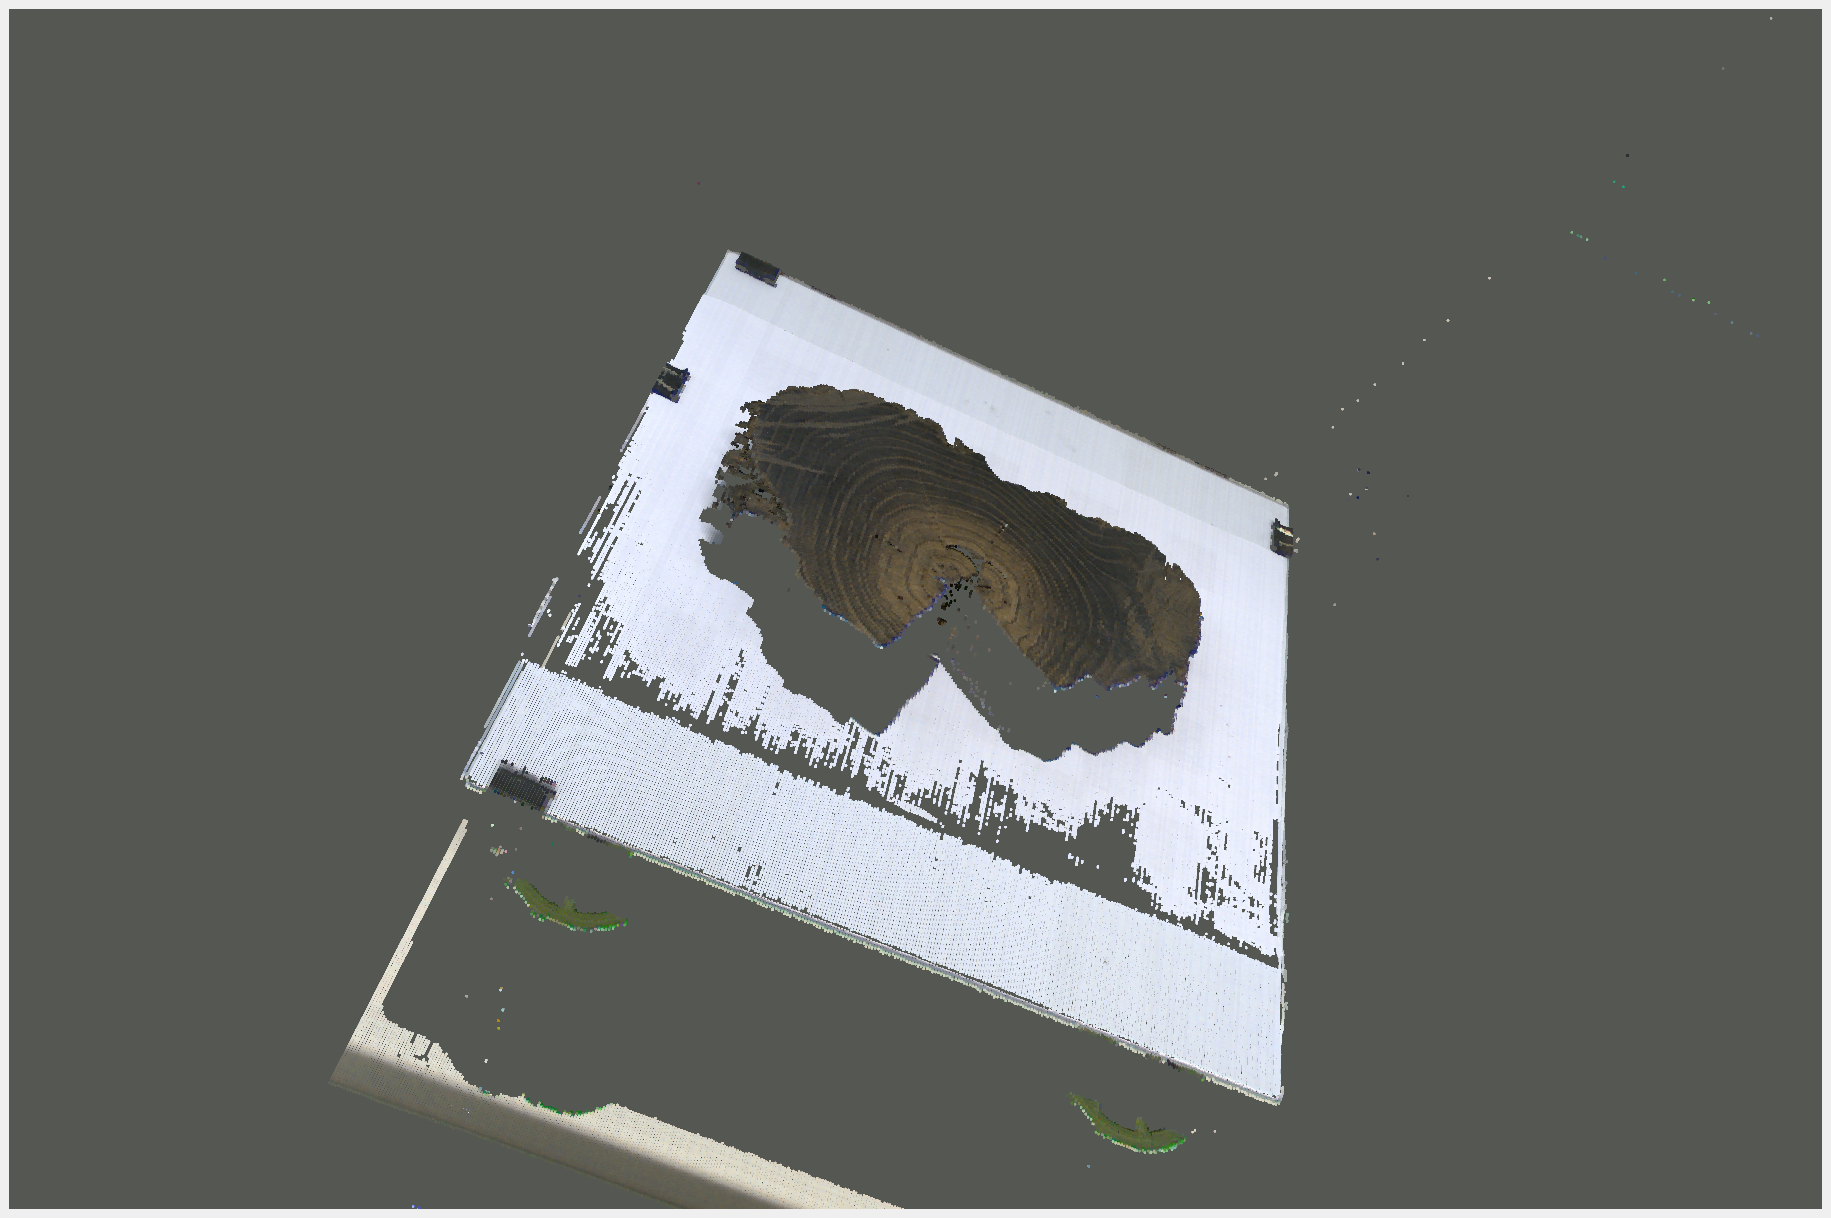
\includegraphics[width=0.49\linewidth]{img/hauptteil/scan-imgs/scan_img_3.png}
			\label{subfig:scan_3}}
		\caption[Qualitative Ergebnisse]{Schachbrett-Kalibrierung mit dem Schachbrett aus verschieden Positionen}
		\label{fig:scan_imgs}
	\end{figure}
	Die aufgenommenen Bilder stammen aus Rviz2. Im Anhang unter \ref{anhang-e} befinden sich weitere Aufnahmen, in dem der Scann näher betrachtet wird. Dabei kann man genau die einzelnen Linien erkennen, die zusammengefügt die komplette Oberflächenrekonstruktion ergeben. 
	\newpage
	
	\subsection{Evaluation}
		
		Der Lasertriangulationssensor wurde nun komplett vorgestellt. Es soll nun eine Evaluation folgen. Dabei wird zuerst eine Methode vorgestellt, die die Genauigkeit eines Scann berechnen kann. Nachdem werden zusätzlich aufgekommene Probleme und Schwierigkeiten erläutert.   
		\subsubsection{Testen von Genauigkeit}
		Ziel ist es die aufgenommene Punktewolke zu testen. Dazu muss das \glqq Ist\grqq{} mit einem \glqq Soll\grqq{} verglichen werden. Hierbei ist es schwierig ein \glqq Soll\grqq{} für einen beliebigen Scann zu finden. Für Beispielsweise Aufnahmen von einem Holzstück oder andere Figuren müsste dann im vornherein schon ein genaues 3D-Modell vorliegen. Daraus ergibt sich, dass zum Vergleichen ein bekanntes Objekt gewählt werden muss. Grundsätzlich soll damit die relative Genauigkeit der Punkte ermittelt werden. Damit ist gemeint, wie genau die Punkte zueinander liegen. Die genaue Position im Raum ist erst einmal unabhängig zu betrachten. Dabei ist es eine gängige Methode das gescannte Objekt in die Punkte des Scann zu fitten un diese am besten zu den Punkten passende Version als \glqq Soll\grqq{} zu verwenden [Acc-Ver] [Multi-View-Stereo]. Dabei ist es Notwendig ein Form zu wählen, die sich in Punkte fitten lässt. Am naheliegendsten sind dabei Geometrische Formen, wie zum Beispiel eine Ebene, eine Linie oder auch eine Kugel. Genau diese drei Formen wurden auch hier zur Genauigkeitsbestimmung gewählt.Die Vorgehensweise demnach ist ein Scann durchzuführen der eine Ebene aufnimmt. In die Punktewolke der Ebene wird dann, ähnlich wie in Kapitel \ref{chap:kalibrierung_extrinsisch} das Finden der Laser-Ebene, eine perfekt passende neue Ebene gefittet. Diese wird als \glqq Soll\grqq{} angesehen. Der eigentliche Vergleich findet dann statt, indem die Abstände der einzelnen Punkte zu der \glqq Soll\grqq-Ebene errechnet werden. Der Durchschnitt dieser Abstände ist der \textit{Mean Squeared Error} und gibt die Genauigkeit an. Um eine höhere Genauigkeit der Messung zu erlangen wird für eine bestimmte Szene dreimal ein Scann durchgeführt. Die gewollte Form wird dann über dein Least-Squares-Algorithmus in die Punkte gefittet. Sobald das geschehen ist, können die Abstände der Punkte zu der Form berechnet werden. Der erste Versuch ist mit einer Linie gemacht worden. Dazu wurde eine einzelne Laserlinie von einer geraden Fläche aufgenommen.  
		
		\begin{table}[h]
			\centering
			\begin{tabular}[h]{c|c|c||c}
				Scann 1 & Scann 2 & Scann 3 & Durchschnitt \\
				\hline
				74,68858 $\mu$m & 85,75119 $\mu$m & 82,05037 $\mu$m & 80,83005 $\mu$m \\
				\hline
			\end{tabular}
			\caption{Messungen einer Linie}
			\label{tab:linie}
		\end{table}
	
		Die zweite Messung betrachtet eine Ebene. Der Versuchsaufbau selbst bietet dazu gute Möglichkeiten, da die Grundlage der Linear-Führung eben ist. Diese wird in einem kompletten Scann-Ablauf aufgenommen. Da durch den Versuchsaufbau auch einzelne Objekte links und recht der Linear-Führung aufgenommen werden (siehe \ref{chap:qual_ergeb}), muss die Punktewolke etwas zugeschnitten werden. In die resultierenden Punkte kann dann eine Ebene gefittet werden. Berücksichtigt werden dann die Abstände der Punkte zu der Ebene.  
		
		\begin{table}[h]
			\centering
			\begin{tabular}[h]{c|c|c||c}
				Scann 1 & Scann 2 & Scann 3 & Durchschnitt \\
				\hline
				0,12192 mm & 0,12159 mm & 0,11337 mm & 0,11896 mm \\
				\hline
			\end{tabular}
			\caption{Messungen einer Ebene}
			\label{tab:ebene}
		\end{table}
	
		Für die dritte Messung wurde eine Kugel benutzt. Der Unterschied zu den vorherigen Messungen ist, dass hier die tatsächliche Größe des Objektes mit evaluiert wird. Beim fitten einer Kugel wird Radius ausgegeben. Die verwendete Kugel hat einen Radius von 5 cm.
	
		\begin{table}[h]
			\centering
			\begin{tabular}[h]{c|c|c||c}
				Scann 1 & Scann 2 & Scann 3 & Durchschnitt \\
				\hline
				0,35608 mm & 0,35462 mm & 0,33945 mm & 0,35005 mm \\
				\hline
				4,80014 cm & 4,80705 cm & 4,80895 cm & 4,80538 cm \\
				\hline
			\end{tabular}
			\caption{Messungen einer Kugel}
			\label{tab:sphere}
		\end{table}
		
		\subsubsection{Probleme und Schwierigkeiten}\label{chap:probleme_schwierigkeiten}
		Bei der Entwicklung und beim Testen des Lasertriangulationssensors sind einige Probleme und Schwierigkeiten aufgetreten. Die ausschlaggebenden sollen hier angesprochen werden.
		
		$\underline{Die \; Beleuchtung}$
		
		Für das Erkennen der Farbinformation ist eine ausreichende Beleuchtung wichtig. Schnell passiert es, dass die Beleuchtung zu dunkel ausfällt und die Farben nicht gut erkennbar sind. Grundsätzlich ist das ein schnell behebbares Problem. Übe Pylon kann die verwendete Basler-Kamera an die Aktuelle Beleuchtung angepasst werden. Das Dilemma zum Thema der Beleuchtung ist viel mehr, dass je heller das Bild wird, um so weniger ist die Laserlinie erkennbar. An hellen Stellen, auch zu sehen bei den Qualitativen Ergebnissen in \ref{chap:qual_ergeb}, wird die Laserlinie nicht mehr erkannt. Dort ist es so hell, das kein ausreichender Unterschied in der Differenz des Bildpaares auffindbar ist. Gerade in \ref{subfig:scan_0} und \ref{subfig:scan_3} ist dieses Problem eindeutig am Rand der Unterlage des Holzes zu sehen. Sobald man die Kamera etwas dunkler Einstellt, werden die Farben des Holzes weniger gut erkannt. Es ist demnach notwendig die Kamera immer an die aktuelle Beleuchtung anzupassen. Die Anpassung muss so eingestellt sein, dass der Laser gut erkannt wird und gleichzeitig die Farben gut erkennbar sind. Ein automatisches Einstellen der Kamera ist bisher nicht implementiert.
		
		$\underline{\ddot{A}nderung \; im \; Bildpaar}$
		
		Der Lasertriangulationssensor ist sehr Anfällig auf jegliche Änderung der Szene, die zwischen den beiden Aufnahmen des Bildpaares stattfinden. Nach Plan darf sich hier nur das Einschalten des Laser ändern. Falls sich etwas anderes in Szene ändert, wird dies eindeutig in der Differenz der Bilder erkennbar sein. Da der Algorithmus immer bei der höchsten Intensität ansetzt ist er grundsätzlich robust und wird den Punkt der Laserlinie wählen. Sobald der Unterschied größer ist, kommt es zu ausschlaggebenden Fehlern. Auch hier ist die Beleuchtung wieder eine Fehlerquelle. Die Kamera kann ein Lichtflackern aufnehmen, welches für das menschliche Auge nicht sichtbar ist. Sobald dann ein Bild heller oder dunkler ausfällt, erhält man ein fehlerhaftes Differenz-Bild.
		
		$\underline{Fehlerquellen \; im \; Versuchsaufbau}$
		
		Als zusätzliche Fehlerquelle ist noch der Versuchsaufbau zu nennen. Die Möglichkeit den verwendeten Schrittmotor anzusteuern ist begrenzt. Hier ist es möglich den Schrittmotor den Befehl sich zu bewegen zu senden. Dabei gibt es kein Feedback, welches erhalten werden kann, sobald die Bewegung abgeschlossen ist. Die Ausführung des Codes muss aber warten, dass die Bewegung tatsächlich abgeschlossen ist. Sonst könne es passieren, dass in der Ausführung der Triangulationssensor davon ausgeht, dass sich die Szene um einen Millimeter weiterbewegt hat, aber die eigentliche Bewegung ist noch nicht abgeschlossen. Die Ausführung und Ermittlung der Punktewolken ist dabei schnell genug , um zweimal innerhalb der Bewegung von einen Millimeter zu erfolgen. Der erste Fehler der hierbei passieren kann, ist, dass die Szene zwischen den Aufnahmen in Bewegung ist und dadurch das Differenz-Bild fehlerhaft ist. Der zweite Fehler ist, dass die Laserlinie in der resultierenden Punktewolke an falscher Position eingefügt wird. Für diese Fehlerquellen wurde der Versuchsaufbau schon so angepasst, dass im Code, nachdem der Befehl für die Bewegung gesendet wurde, eine Sekunde gewartet wird. So ist die Bewegung sicher abgeschlossen, bevor die nächsten Aufnahmen gemacht werden. Nachteil dadurch ist, dass der Scann vergleichsweise langsam aufgenommen wird. Trotzdem bleibt ein kleiner Fehler in der Position. Beim Anhängen der neuen Laserlinie wird genau ein Millimeter in x-Richtung aufaddiert. Hierbei ist ohne größeren Aufwand nicht überprüfbar, ob sich die Linear-Führung genau um einen Millimeter bewegt. Das hängt davon ab, wie genau der Schritt-Motor kalibriert ist. Die Varianz der Laserlinie ist gering und kann somit vernachlässigt werden. Es ist wahrscheinlicher, dass die Kalibrierung des Schritt-Motors für kleine Fehler verantwortlich ist. Diese Fehler können sich in der Oberflächenrekonstruktion aufaddieren und dazu führen, dass die gesamte Punktewolke in x-Richtung fehlerhaft ist. Hiermit wäre auch die der fehlerhafte Radius der gescannten Kugel erklärbar.
		
		$\underline{Spiegelung \; und \; schlechte \; Reflektion \; der \; Laserlinie}$
		
		Für einen Lasertriangulationssensor ist grundlegend vorausgesetzt, dass die Laserlinie auf den Objekt sichtbar ist. Das bedeutet, dass sie gut reflektiert wird. Wenn das nicht der Fall ist, kommt es zu Fehlern. Durchsichtige oder nihct reflektierende Oberflächen können vom Sensor nicht erfasst werden.      
\clearpage

% ----------------------------------------------------------------------------------------------------------
% Fazit
% ----------------------------------------------------------------------------------------------------------
% ----------------------------------------------------------------------------------------------------------
% Das Fazit
% ----------------------------------------------------------------------------------------------------------
\section{Zusammenfassung}\label{zusammenfassung}
	Zusammengefasst lässt sich festhalten, dass der Lasertriangulationssensor an sich erwartungsgemäß gut funktioniert. Eine einzelne Laserlinie lässt sich mit hoher Genauigkeit als Punktewolke aus Kamerasicht rekonstruieren. Dabei ist die Anwendung mit ROS2 ausführbar. Die größte Fehlerquelle war der Versuchsaufbau selbst. Da nicht genau die Position der Linear-Führung herausgefunden werden kann, können die neuen Laserlinien nie perfekt zu der Gesamt-Punktewolke angefügt werden. Die Implementierung mit ROS2 ist jedoch sehr gut anpassbar. Für die Steuerung des Versuchsaufbau ist grundsätzlich nur der Client zuständig. Die Gesamt-Punktewolke wird vom Sensor selbst erstellt. In der aktuellen Implementation werden die neuen Punkte immer um einen Millimeter in x-Richtung verschoben. Problem war dabei, dass nicht verifiziert werden kann, ob sich die Linear-Führung um genau einen Millimeter bewegt. Wenn man eine Änderung des Versuchsaufbau in Erwägung zieht, muss also der Client selbst und das Anfügen der neuen Punkte in der Scanner-Klasse angepasst werden. Sonst kann der Sensor problemlos weiterverwendet werden. Gerade die entwickelte Bibliothek in Python ist sehr robust. Natürlich ist diese an das verwendetet Kalibrierverfahren angepasst. Hier ist eine Anpassung aufwändiger. Dazu lässt sich jedoch sagen, dass die Genauigkeit einer einzelnen Linie sehr gut ist. Da die Genauigkeit direkt aus der Kalibrierung resultiert, muss im Umkehrschluss die Kalibrierung auch sehr erfolgreich sein. \newline
	Wichtig hervorzuheben ist, dass der entwickelte Sensor an sich immer nur eine einzelne Laserlinie in eine Punktewolke übersetzt. Herkömmliche RGB-D-Kameras können sofort eine ganze Oberfläche mit einer Aufnahme als Punktewolke liefern. Das liegt daran, dass RGB-D-Kameras zumeist über zwei bis drei Kameras verfügen. Zusätzlich benutzten sie nicht nur eine Laserlinie, sondern ganzes Muster an beispielsweise Infrarot-Licht. Ein Beispiel dafür ist die „Intel RealSense d415“ selbst. Der hier entwickelte Lasertraingulationsensor besitzt nur eine Kamera und arbeitet mit einer Laserlinie. Ausgabe ist also immer der Querschnitt des aktuellen Objektes. Trotzdem passt der Sensor damit immer noch zum Gesamtprojekt, die Automatisierung der Jahrringmessstation. Hier soll ein Roboterarm zum Einsatz kommen. Dieser Arm kann sich über das Objekt bewegen. Dabei können genau Befehle an den Arm gesendet werden, um zum Beispiel sich auch genau ein Millimeter zu bewegen. Hinzu kommt, dass bei einem Roboter die Transformationen von der eingebauten Kamera zu einem festgelegten Weltkoordinatensystem bekannt sind. Damit können die errechneten Punkte in das Weltkoordinatensystem transformiert werden und gleich ihren genauen Platz einnehmen. Der Versuchsaufbau, bestehen aus der Linear-Führung und den Arduino mit CNC-Shield ist nur zum Testen des Scannen einer kompletten Oberfläche entwickelt wurden. Das eigentliche Ziel ist jedoch die Anbringung des Sensors an einen Roboterarm. Dafür sind Anpassungen im steuernden Client und in dem Zusammenfügen der Punktewolke notwendig. \newline
	Intern läuft die Zusammenarbeit von ROS2 un der Python-Bibliothek problemlos. Für aufkommende Fehler wurde eine Weiterbehandlung eingebaut. Die hier gemeinten Fehler beziehen sich auf Aufnahmen der Kamera, die beispielsweise kein Schachbrett oder ChArUco-Board zeigen, aber zu Kalibrierung verwendet werden sollen. Also allgemeine Fehler der Bildverarbeitung bei der Kalibrierung. Hierbei wird erkannt, ob eine erfolgreiche Kalibrierung mit den Aufnahmen durchgeführt werden konnte. Falls nicht, wird sie als fehlgeschlagen deklariert. Über das Feedback des aufgerufenen Kalibrier-Service erfährt dann der Benutzer, wo ein Fehler gefunden wurde. Zusätzlich wird bei einer vermeintlich erfolgreichen Kalibrierung die entstandene Laser-Ebene als Punktewolke an Rviz2 geschickt. So kann deren Richtigkeit vom Benutzer überprüft werden. Dabei werden auch die Bilder, die der Sensor zur Kalibrierung aufgenommen hat abgespeichert und können eingesehen werden. Somit erhält der Nutzer genug Informationen über den Erfolg der Kalibrierung. 
      
\clearpage

% ----------------------------------------------------------------------------------------------------------
% Ausblick
% ----------------------------------------------------------------------------------------------------------
% ----------------------------------------------------------------------------------------------------------
% Der Ausblick
% ----------------------------------------------------------------------------------------------------------
\section{Ausblick}\label{ausblick}
	
	Um entstandene Fehler und Schwierigkeiten zu umgehen oder zu beheben gibt es verschiedene Möglichkeiten. Die erste und wichtigste Erweiterung ist es, den Versuchsaufbau anzupassen oder zu ersetzen. Das größte Problem ist die Umsetzung der neuen Position der Laserlinie in die richtige Position der digitalen Punktewolke. Momentan wird sich auf die Genauigkeit des verwendeten Schrittmotors verlassen. So geht man davon aus, dass sich die Linear-Führung um genau einen Millimeter bewegt, um diesen dann bei der neuen Punktewolke mit einzurechnen. Weniger fehleranfällig wäre eine Möglichkeit, die Verschiebung der Punkte zu berechnen. Dazu könnten man die Grundlage des Objektes auf der Linear-Führung eine von der Kamera erkennbare Markierung versehen. Beispielsweise ein ArUco-Marker. Durch die durchgeführte Kalibrierung ist es möglich, ein Koordinatensystem auf den Marker zu legen. Rotation und Translation sind dabei bekannt. Die Punkte der Laserlinie liegen dann in diesem Koordinatensystem, welches die Linear-Führung beschreibt. Als zusätzlicher Schritt müssen die Punkte dann in das Koordinatensystem transformiert werden, in dem die Ebene-Gleichung definiert ist. Alle restlichen Schritte sind bereits implementiert. Durch diese Anpassung wird die neue Punktewolke immer exakt angefügt. Die Länge der Schritte des Schrittmotors müssen dann nur so angepasst werden, dass das Objekt möglichst genau aufgenommen werden kann. Anforderungen an den Aufbau wären dann zusätzlich, dass der verwendete Marker immer auf jeden Bild erkennbar sein muss. \newline
	Grundsätzlich sollte aber das eigentliche Ziel sein, den Versuchsaufbau abzuschaffen und den Sensor an einen Roboterarm anzubringen. Die Bewegung ist ausgelagert und wird vom Client gesteuert. Dieser wird demnach auch die Steuerung des Roboterarms übernehmen. Hier muss der Client an das Gesamtprojekt angepasst werden. \newline
	Ein weiteres Problem ist das der Beleuchtung. Hier könnte man nach Vorbild moderner RGB-D-Kameras eine zusätzliche Kamera verwenden. Somit ist eine Kamera für das Aufnehmen der Laserlinie zuständig und eine andere nimmt ein Bild für die Farbinformationen auf. Vorteil davon ist, dass beide Kameras für ihren eigenen Zweck angepasst und eingestellt werden können. Damit umgeht man das Dilemma, dass die Laserlinie schlechter erkennbar wird, um so heller die Oberfläche beleuchtet ist. Ein neu aufkommendes Problem dabei ist, dass die beiden Kameras nicht an der selben Stelle montiert sind. Das bedeutet, dass es zu Fehlern der Farbe kommen kann, da die Positionen der Pixel in den Aufnahmen nicht unbedingt übereinstimmen. Dieses Problem kann behoben werden, indem man die bekannten Transformationen benutzt, um die möglichst genauste Repräsentation eines errechneten 3D-Punktes als Pixel zu finden. Voraussetzung dafür ist die Kalibrierung beider Kameras. Alternativ zur zusätzlichen Kamera wäre die Aufnahme eines dritten Bildes. Das Bildpaar zum Erkennen der Laserlinie behält seine Funktion bei. Hinzu kommt eine dritte Aufnahme die unter besserer Beleuchtung aufgenommen wird. Dazu müsste man dem Aufbau eine passende Lichtquelle hinzufügen, vergleichbar mit dem Blitzlicht einer Kamera. Diese dritte Aufnahme wird dann über die herkömmliche Methode zum Finden der Farbinformationen weiterverwendet. Vorteil dieser Methode ist, dass der Scanner nun unabhängig von anderer Beleuchtung ist. Alles benötigte Licht wird nun vom Scanner selbst in einer definierten Helligkeit produziert.
	
	Der bisherige Ausblick geht davon aus, dass die Methodik der Lasertriangulation mit einem Linienlaser beibehalten wird. Erwähnenswert sind hierbei Alternativen, wie Stereo Vision oder auch Time of Flight. Die Genauigkeiten eines Scanns mit diesen Methoden und ob diese zu dem Gesamtprojekt passend sind wurde in dieser Arbeit nicht untersucht. Grundsätzlich ist es Sinnvoll sich jedoch weiter im Bereich der Triangulation aufzuhalten, da Time of Flight ein sehr unterschiedlicher Ansatz ist, 3D-Informationen zu erhalten. \newline
	Die zugrunde liegende Aufgabe war es eine 3D-Rekonstruktion eines Objektes mit Farbinformationen zu erhalten. Diese Aufgabe erfüllt der entwickelte Sensor ausreichend. Die 3D-Informationen werden aus Kamerasicht geliefert. Mithilfe der Farbinformationen können passende Pfade zum abfahren des Holzes ausgewählt werden      	
\cleardoubleemptypage

% ----------------------------------------------------------------------------------------------------------
% Anhang
% ----------------------------------------------------------------------------------------------------------
\begin{appendix}
	
	\section{Anhang}
		\subsection{Anhang A}\label{anhang-a}
		\begin{figure}[h]
			\centering
			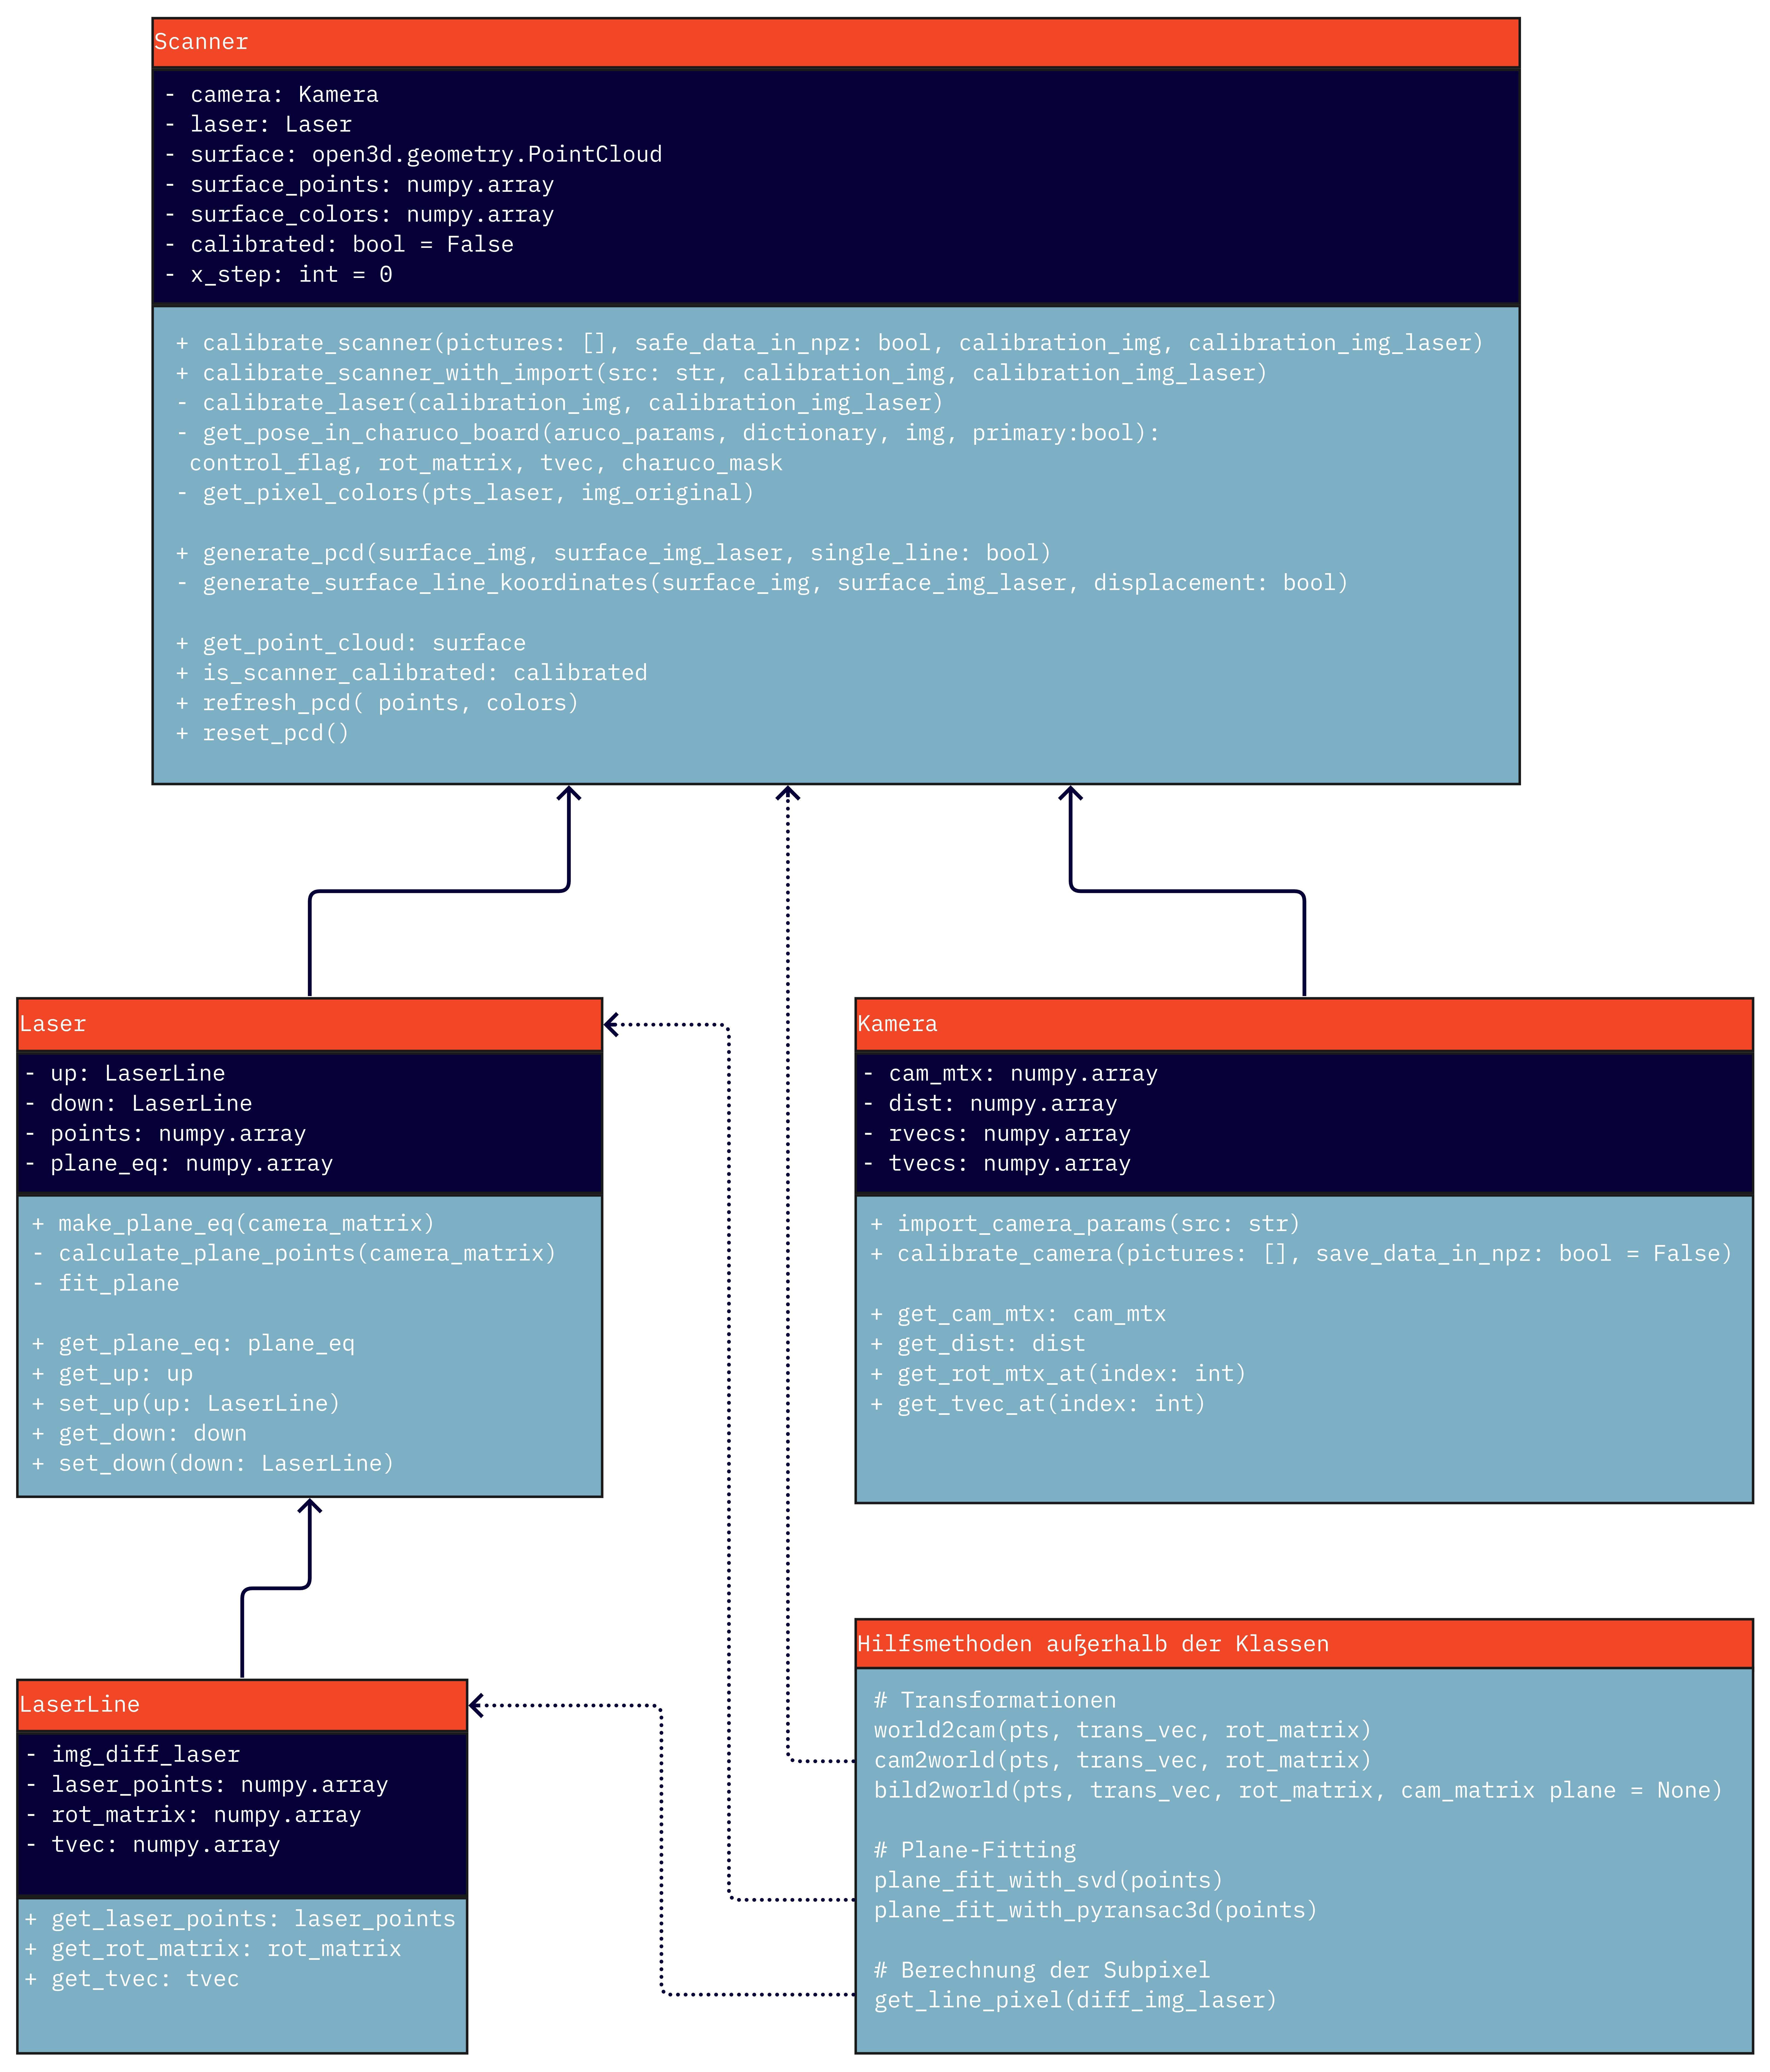
\includegraphics[width=0.93\linewidth]{img/anhang/UML_surface_scanner.jpg}
			\caption{UML-Klassendiagramm des Lasertriangulationssensor}
			\label{fig:uml_all}
		\end{figure}
		\newpage
		\subsection{Anhang B}\label{anhang-b}
		
		\clearpage
		
		\subsection{Anhang C}\label{anhang-c}
		
		\clearpage
		
\end{appendix}
\cleardoublepage



% ----------------------------------------------------------------------------------------------------------
% Abbildungsverzeichnis
% ----------------------------------------------------------------------------------------------------------
\ohead{Abbildungsverzeichnis}
\listoffigures
\clearpage

% ----------------------------------------------------------------------------------------------------------
% Tabellenverzeichnis
% ----------------------------------------------------------------------------------------------------------
\ohead{Tabellenverzeichnis}
\listoftables
\clearpage

% ----------------------------------------------------------------------------------------------------------
% Codeverzeichnis
% ----------------------------------------------------------------------------------------------------------
\ohead{Quellcodeverzeichnis}
\renewcommand{\lstlistlistingname}{Quellcodeverzeichnis}
\clearpage

\lstlistoflistings
\clearpage

% ----------------------------------------------------------------------------------------------------------
% Abkuerzungen
% ----------------------------------------------------------------------------------------------------------
\ohead{Abkürzungsverzeichnis}
\section*{Abkürzungsverzeichnis}
\addcontentsline{toc}{section}{Abkürzungsverzeichnis}
\begin{acronym}[ITI] % laengste Abkuerzung steht in eckigen Klammern
	\setlength{\itemsep}{-\parsep} % geringerer Zeilenabstand
	\acro{ITI}{Institut für Technik und Informatik}
	\acro{MNI}{Mathematik, Naturwissenschaften und Informatik}
	\acro{THM}{Technische Hochschule Mittelhessen}
	%\acro{}
	
\end{acronym}
\clearpage
\ohead{\leftmark}

%TODO: Fix Floating Numbering 
% ----------------------------------------------------------------------------------------------------------
% Literaturverzeichnis
% ----------------------------------------------------------------------------------------------------------

%\bibliographystyle{literatur}{unsrtdin}
%\raggedright
%\bibliography{literatur}{bib/literatur}{Literaturverzeichnis}
%\clearpage
%
%% ----------------------------------------------------------------------------------------------------------
%% Datenblattverzeichnis
%% ----------------------------------------------------------------------------------------------------------
%
%\bibliographystyle{datenblatt}{unsrtdin}
%\raggedright
%\bibliography{datenblatt}{bib/datenblatt}{Datenblattverzeichnis}
%\clearpage

% ----------------------------------------------------------------------------------------------------------
% Bildverzeichnis
% ----------------------------------------------------------------------------------------------------------

\bibliographystyle{all}{unsrtdin} % apalike
\raggedright


\bibliography{all}{bib/all}{Quellenverzeichnis}
\clearpage

% ----------------------------------------------------------------------------------------------------------
% Eidesstattliche Erklärung
% ----------------------------------------------------------------------------------------------------------
\thispagestyle{empty}
% ----------------------------------------------------------------------------------------------------------
% Eidesstattliche Erklärung
% ----------------------------------------------------------------------------------------------------------
\section*{Eidesstattliche Erklärung}
	\vspace{1cm}
	Hiermit versichere ich, die vorliegende Arbeit selbstständig und unter ausschließlicher Verwendung der angegebenen Literatur und Hilfsmittel erstellt zu haben.
	
	Die Arbeit wurde bisher in gleicher oder ähnlicher Form keiner anderen Prüfungsbehörde vorgelegt und auch nicht veröffentlicht.
	
	\vspace{2cm}
	\parbox{6cm}{\centering Gießen, 25.05.2022\hrule
		\strut \centering\footnotesize Ort, Datum} \hfill\parbox{6cm}{\hrule
		\strut \centering\footnotesize Unterschrift}

\clearpage

% ----------------------------------------------------------------------------------------------------------
% Index
% ----------------------------------------------------------------------------------------------------------
%\cleardoublepage
%\printindex

\end{document}
